\chapter{Hypothesis Tests}
\label{chapterHypothesisTests}
\index{Hypothesis tests}

Hypothesis testing is a very important topic in statistical inference. When carrying out a hypothesis test, a claim about the value of a parameter is tested using statistical methods. In Chapter $\ref{chapterConfidenceIntervals}$, we discussed how to use confidence intervals to draw conclusions about the value of the parameter based on the bounds of a constructed interval. By using hypothesis testing, we are able to take this a step further by quantifying the strength of our conclusion with a probability statement.\\

The mathematical background behind a hypothesis test begins with a decision rule. 
%A \textit{decision rule} maps an observed value to an action. 
A \textit{decision rule} is a rule that is used to decide on a conclusion to make in a hypothesis test based on
based on a calculated value obtained from data.
\index{Decision rule}
In the instance of hypothesis testing, the value of a test statistic determines whether we accept our hypothesis or reject it. A test statistic is a value calculated using sample data. The mathematical formulae underlying test statistics are derived using decision rules and the famous likelihood ratio test, which are covered in greater detail in advanced undergraduate or graduate courses in mathematical statistics.\\

We will skip the mathematical derivation of a hypothesis test and get right into the procedure of conducting them. This makes the process of conducting a hypothesis test somewhat algorithmic in nature.

\begin{algorithm}[]
Steps involved in conducting a hypothesis test:

\begin{enumerate}
\item	State the null and alternative hypothesis.
\item	Find the appropriate test statistic.
\item	Find the p-value
\item	Compare p-value to a level of significance ($\alpha$).
\item	Make a conclusion.
\end{enumerate}
\end{algorithm}


\noindent
{\em \underline{1. State the null and alternative hypothesis} }\\

\noindent
The first step in hypothesis testing is to state the null and alternative hypothesis. The null hypothesis is the conservative or skeptical belief and the alternative hypothesis is the claim we are testing. The alternative is usually a researchers' belief. The null hypothesis is represented by $H_{0}$  and the alternative hypothesis is represented by $H_{a}$

\begin{definition}[Null and Alternative Hypothesis]	
\begin{tabular}{l c m{14.75cm} }
$H_{0}$	& : &	Null hypothesis	\\	\index{Hypothesis!Null hypothesis}
		&   &	Represents either a skeptical or conservative perspective on a claim to
			be tested.\\
\hfill\\
$H_{a}$	& : &	Alternative hypothesis	\\	\index{Hypothesis!Alternative hypothesis}
		&   &	Represents an alternative claim or alternative belief 
			under consideration. 
			Usually considers a range of possible values for a parameter.
\end{tabular}
\end{definition}



\begin{nt}
Some textbooks use the notation $H_{1}$ to refer to the alternative hypothesis. We will be using $H_{a}$ consistently throughout this text.
\end{nt}

\noindent
When conducting a hypothesis test, we operate under the assumption that $H_{0}$ is true. Our goal is to find evidence in support of $H_0$ or against $H_0$. 

\begin{definition}[Types of Hypothesis Tests]	\index{Hypothesis tests!Types of}
Suppose $\gamma$ is the parameter we are interested in and $\gamma_{0}$ is the hypothesized value of 
$\gamma$ under the null hypothesis. 
The 3 possible hypothesis tests we can perform are:\\
	
%\parbox{10cm}{
	\begin{enumerate}
	\item	$H_{0} : \gamma = \gamma_{0}$ ~vs.~ $H_{a}  : \gamma > \gamma_{0}$
		\label{hyptestgeq}
	\item	$H_{0} : \gamma = \gamma_{0}$ ~vs.~ $H_{a}  : \gamma < \gamma_{0}$
		\label{hyptestleq}
	\item	$H_{0} : \gamma = \gamma_{0}$ ~vs.~ $H_{a}  : \gamma \neq \gamma_{0}$
		\label{hyptestneq}
	\end{enumerate}
%}
\hfill\\
\noindent
Hypothesis tests $\ref{hyptestgeq}$ and $\ref{hyptestleq}$ are referred to as  one-sided or one-tailed tests. Hypothesis test $\ref{hyptestneq}$ is referred to as a two-sided or two tailed test. This test may also be referred to as a non-directional test.
\end{definition}

\begin{nt}
We will always write the null hypothesis as an equality (``$=$'')
and the alternative hypothesis as a strict inequality (either ``$<$'' or ``$>$''.
\end{nt}


\hfill\\


\noindent
{\em \underline{2. Find the Appropriate Test Statistic} }\\

\begin{definition}[Test Statistic]	\index{Statistic!Test statistic}
A statistic calculated from sample data that is used to conduct a hypothesis test.
\end{definition}

\noindent
The test statistic we calculate depends on the information available as well as the assumed value of the parameter under the null hypothesis.

\begin{skeleton}
General form of a test statistic:
	\begin{equation}\label{equationGeneralFormTestStat}
	\text{Test Statistic} = \frac{ \text{(a statistic)} -  \text{(hypothesized value of parameter)} }{ \text{(standard error of statistic)} }
	\end{equation}
\end{skeleton}

The calculated test statistic follows a certain reference distribution. In this course the reference distributions we will be using are either the standard normal distribution or the $t-$distribution.

\begin{nt}
A statistic as basic as the sample mean $\bar{x}$ on its own 
can also be used as a test statistic, 
however this is not common practice and many test statistics 
are in the form of $\ref{equationGeneralFormTestStat}$.
\end{nt}


\hfill\\
\noindent
{\em \underline{3. Find the p-value} }\\

\noindent
P-values are used to quantify the strength of the evidence supporting 
(or against) the null hypothesis via a probability statement. The p-value is calculated using the test statistic and is dependent on the form of the alternative hypothesis. We formally define a p-value in definition $\ref{definitionPValue}$ but caution the reader that it is difficult to understand the definition of a p-value immediately and a proper comprehension of p-values may take time.

\begin{definition}[P-value]\label{definitionPValue}	\index{P-value}
Assuming that $H_{0}$ is true, the p-value is the probability of calculating a test statistic at least as extreme as the one computed using sample data solely by chance.
\end{definition}

Recall that a test statistic is calculated using sample data and the assumed value of the parameter under the null hypothesis. A p-value is the probability of calculating the same test statistic or a test statistic that is even more unlikely than the one just calculated by pure chance and without any other external factors. If the p-value is extremely small, it is unlikely that the assumed value of the parameter under the null hypothesis is correct.\\

Figures $\ref{figureSmallPvalHaLess}$,
$\ref{figureSmallPvalHaGreater}$,
$\ref{figureLargePvalHaLess}$,
$\ref{figureLargePvalHaGreater}$
and
$\ref{figurePvalHaNeq}$.
provide some examples of p-values when the reference distibution
is either the normal distribution of the $t-$distribution.
The shaded area represents the p-value.

\hfill
\begin{figure}[H]
\centering
\begin{minipage}{.450\textwidth}
	\underline{Suppose $H_{a}: \gamma < \gamma_{0}$}\\
	\hfill\\
	%\scalebox{1.50}{
	\begin{tikzpicture}[scale=1.6]
	% define normal distribution function 'normaltwo'
	\def\normaltwo{\x,{ 5*(1/2.50662827463)*exp(-((\x-0)^2)/1) }}
	% input y parameter
	\def\y{-1.0}
	\def\fy{ 5*(1/2.50662827463)*exp(-((\y-0)^2)/1) }
	% Shade orange area underneath curve.
	\fill [fill=oiB7] (-2.3,0) -- plot[smooth, domain= -2.3:-1 ] (\normaltwo) -- ({\y},0) -- cycle;
	% Draw and label normal distribution function
	\draw[color=oiB, smooth, domain=-2:2] plot (\normaltwo) node[right] {};
	% Add dashed line dropping down from normal.
	\draw[dashed] ({\y},{\fy}) -- ({\y},0) node[below, text width=1.5cm, align=center] {\em \centering test statistic};
%	\draw[<-,thick] (0.75,0.05) -- (1.6,0.2) node[right,yshift=0.3cm]
%    {\begin{tabular}{l} $\alpha=0.05$ \\ (Type I error rate) \end{tabular}};

	\draw[->] (-2.25,0) -- (2.25,0) node[right] {};
	\end{tikzpicture}
	%}
\vspace{-0.25cm}
\caption{	A p-value in the small tail of a reference distribution when the alternative is that
		the parameter is less than a hypothesized value.}
\label{figureSmallPvalHaLess}
\end{minipage}
\hspace*{0.25cm}
\begin{minipage}{.450\textwidth}
	\underline{Suppose $H_{a}: \gamma > \gamma_{0}$}\\
	\hfill\\
	%\scalebox{1.50}{
	\begin{tikzpicture}[scale=1.6]
	% define normal distribution function 'normaltwo'
	\def\normaltwo{\x,{ 5*(1/2.50662827463)*exp(-((\x-0)^2)/1) }}
	% input y parameter
	\def\y{+1.0}
	\def\fy{ 5*(1/2.50662827463)*exp(-((\y-0)^2)/1) }
	% Shade orange area underneath curve.
	%\fill [fill=oiB7] (-3,0) -- plot[smooth, domain= -3:-1 ] (\normaltwo) -- ({\y},0) -- cycle;
	\fill [fill=white] (-2.3,0) -- plot[smooth, domain= -2.3:-1 ] (\normaltwo) -- ({\y},0) -- cycle;
	\fill [fill=oiB7] (1,0) -- plot[smooth, domain= 1:2.3 ] (\normaltwo) -- ({\y},0) -- cycle;
	% Draw and label normal distribution function
	\draw[color=oiB, smooth, domain=-2:2] plot (\normaltwo) node[right] {};
	% Add dashed line dropping down from normal.
	\draw[dashed] ({\y},{\fy}) -- ({\y},0) node[below, text width=1.5cm, align=center] {\em  test statistic};
	\draw[->] (-2.25,0) -- (2.25,0) node[right] {};
	\end{tikzpicture}
	%}
\vspace{-0.25cm}
\caption{	A p-value in the small tail of a reference distribution when the alternative is that
		the parameter is greater than a hypothesized value.}
\label{figureSmallPvalHaGreater}
\end{minipage}
\end{figure}

%\hfill\\[-2.0em]
\begin{figure}[H]
\centering

\begin{minipage}{.450\textwidth}
	\underline{Suppose $H_{a}: \gamma < \gamma_{0}$}\\
	\hfill\\
	%\scalebox{1.50}{
	\begin{tikzpicture}[scale=1.6]
	% define normal distribution function 'normaltwo'
	\def\normaltwo{\x,{ 5*(1/2.50662827463)*exp(-((\x-0)^2)/1) }}
	% input y parameter
	\def\y{+1.0}
	\def\fy{ 5*(1/2.50662827463)*exp(-((\y-0)^2)/1) }
	% Shade orange area underneath curve.
	%\fill [fill=oiB7] (-3,0) -- plot[smooth, domain= -3:-1 ] (\normaltwo) -- ({\y},0) -- cycle;
	\fill [fill=oiB7] (-2.3,0) -- plot[smooth, domain= -2.3:+1 ] (\normaltwo) -- ({\y},0) -- cycle;
	\fill [fill=white] (1,0) -- plot[smooth, domain= 1:2.3 ] (\normaltwo) -- ({\y},0) -- cycle;
	% Draw and label normal distribution function
	\draw[color=oiB, smooth, domain=-2:2] plot (\normaltwo) node[right] {};
	% Add dashed line dropping down from normal.
	\draw[dashed] ({\y},{\fy}) -- ({\y},0) node[below, text width=1.5cm, align=center] {\em  test statistic};
	\draw[->] (-2.25,0) -- (2.25,0) node[right] {};
	\end{tikzpicture}
	%}
\vspace{-0.25cm}
\caption{	A p-value in the small tail of a reference distribution when the alternative is that
		the parameter is less than a hypothesized value.}
\label{figureLargePvalHaLess}
\end{minipage}
\hspace*{0.25cm}
\begin{minipage}{.450\textwidth}
	\underline{Suppose $H_{a}: \gamma > \gamma_{0}$}\\
	\hfill\\
	%\scalebox{1.50}{
	\begin{tikzpicture}[scale=1.6]
	% define normal distribution function 'normaltwo'
	\def\normaltwo{\x,{ 5*(1/2.50662827463)*exp(-((\x-0)^2)/1) }}
	% input y parameter
	\def\y{-1.0}
	\def\fy{ 5*(1/2.50662827463)*exp(-((\y-0)^2)/1) }
	% Shade orange area underneath curve.
	\fill [fill=white] (-2.3,0) -- plot[smooth, domain= -2.3:-1 ] (\normaltwo) -- ({\y},0) -- cycle;
	\fill [fill=oiB7] (-1,0) -- plot[smooth, domain= -1:2.3 ] (\normaltwo) -- ({\y},0) -- cycle;
	% Draw and label normal distribution function
	\draw[color=oiB, smooth, domain=-2:2] plot (\normaltwo) node[right] {};
	% Add dashed line dropping down from normal.
	\draw[dashed] ({\y},{\fy}) -- ({\y},0) node[below, text width=1.5cm, align=center] {\em \centering test statistic};
	\draw[->] (-2.25,0) -- (2.25,0) node[right] {};
	\end{tikzpicture}
	%}
\vspace{-0.25cm}
\caption{	A p-value in the large tail of a reference distribution when the alternative is that
		the parameter is greater than a hypothesized value.}
\label{figureLargePvalHaGreater}
\end{minipage}
\end{figure}


%\hfill\\
\begin{figure}[H]
	\underline{Suppose $H_{a}: \gamma \neq \gamma_{0}$}\\
	\hfill\\
\centering
%\scalebox{1.6250}{
	\begin{tikzpicture}[scale=1.6]
	% define normal distribution function 'normaltwo'
	\def\normaltwo{\x,{ 5*(1/2.50662827463)*exp(-((\x-0)^2)/1) }}
	% input y parameter
	\def\y{-1.0}
	\def\fy{ 5*(1/2.50662827463)*exp(-((\y-0)^2)/1) }
	\def\z{+1.0}
	\def\fz{ 5*(1/2.50662827463)*exp(-((\y-0)^2)/1) }
	% Shade orange area underneath curve.
	\fill [fill=oiB7] (-2.5,0) -- plot[smooth, domain= -2.5:-1 ] (\normaltwo) -- ({\y},0) -- cycle;
	\fill [fill=oiB7] (1,0) -- plot[smooth, domain= 1:2.5 ] (\normaltwo) -- ({\z},0) -- cycle;
	% Draw and label normal distribution function
	\draw[color=oiB, smooth, domain=-2:2] plot (\normaltwo) node[right] {};
	% Add dashed line dropping down from normal.
	%\draw[dashed] ({\y},{\fy}) -- ({\y},0) node[below, text width=1.55cm, align=center] 
	\draw[dashed] ({\y},{\fy}) -- ({\y},0) node[below, text width=1.7cm, align=center] {\vspace*{-0.25cm}\[-\left\lvert \parbox{1.30cm}{\em\centering test statistic}\right\rvert \]};
	\draw[dashed] ({\z},{\fz}) -- ({\z},0) node[below, text width=1.7cm, align=center] {\vspace*{-0.25cm}\[+\left\lvert \parbox{1.30cm}{\em\centering test statistic} \right\rvert\]};
	\draw[->] (-2.25,0) -- (2.25,0) node[right] {};
	\end{tikzpicture}
%}
\vspace{-0.25cm}
\caption{	The p-value in the area in the extreme tails of a reference distribution when the alternative is that
		the parameter is not equal to a hypothesized value.}
\label{figurePvalHaNeq}
\end{figure}


\begin{nt}
Since the p-value is a probability it must be a value between 0 and 1.
\end{nt}


\hfill\\
\noindent
{\em \underline{4. Compare with a Level of Significance ($\alpha$)} }\\

\noindent
We compare the p-value with a level of significance (or significance level), $(\alpha)$. The level of significance can be considered as a tolerance level used to determine whether we have sufficient evidence to reject the null hypothesis or not. Formally,

\begin{definition}[Level of Significance ($\alpha$)]	\index{Level of significance}
The probability of rejecting the null hypothesis when it is actually true.
\end{definition}

The level of significance is usually pre-determined before a 
statistical test is performed. If multiple tests are performed on the same data set, we typically use the same value of $\alpha$ for all tests in order to obtain consistent results.

\begin{nt}
If $\alpha$ is not specified, we usually take the default value of $\alpha = 0.05$.
\end{nt}

We can also decide on a level of significance after we calculate the 
p-value, however this is not usually done as it is considered bad practice. Choosing a level of significance after calculating a p-value can result in the abuse and manipulation of statistical tests.


\hfill\\
\noindent
{\em \underline{5. Make a Conclusion} }\\

\noindent
The conclusion we make depends on the p-value calculated and the level of significance.

\begin{rules}[Making a Conclusion on a Hypothesis Test]
\label{ruleConclusionHypTest}
%\begin{center}

\begin{tabular}{lcl}
p-value $> \alpha$	&	$\Longrightarrow$	& 	Evidence supports $H_{0}$.				\\
				&					&	Do not reject $H_{0}$, conclude $H_{0}$.		\\
%				&					&	Conclude $H_{0}$						\\
\hfill\\
p-value $< \alpha$	&	$\Longrightarrow$	& 	Evidence against $H_{0}$.				\\
				&					&	Reject $H_{0}$, conclude $H_{a}$.			\\
\end{tabular}
%\end{center}
\end{rules}

\noindent
The manner in which we make a conclusion for hypothesis tests
is always the same.

\begin{nt}
A common mistake that students make is to refer back to the alternative
hypothesis when they decide the manner in which to make a conclusion.
Once we have the p-value we follow rule $\ref{ruleConclusionHypTest}$.
There is no need to refer back to check the sign of the alternative hypothesis.
\end{nt}
In Chapter $\ref{chapterConfidenceIntervals}$, we stressed the importance of using careful language when drawing conclusions on confidence intervals. This also extends to hypothesis testing. We cannot conclude tests by stating that the null hypothesis is \textit{definitely} correct or that the null hypothesis is \textit{definitly} wrong as this would imply that we are completely certain of our result. When concluding hypothesis tests, the statement we make is based on probability so there is always a chance that we have made an error (see section $\ref{sectionErrors}$). Furthermore, due to the nature of random sampling, we may have obtained a sample that is not representative of the true population. In this case, a misleading test statistic would be calculated and lead us to draw the wrong conclusions about the population. There may also be hidden covariates that are not evident (i.e. there may be a hidden relationship between the data and other factors that we are not aware of). As such we make conclusions by stating that the evidence 
\textit{suggests} we should either support or reject the null hypothesis. If we reject the null hypothesis, we conclude the alternative hypothesis since as it is the only other choice available to us.

\begin{nt}
Hypothesis tests use an evidence based approach to make conclusions,
hence we make conclusions by stating that either the
evidence supports the null or the evidence is against the null hypothesis.\\

If we have a very small p-value, we can state that we have strong evidence
against the null hypothesis and if we have a large p-value we can state
that we have strong evidence supporting the null hypothesis.
\end{nt}



\section{One Sample Hypothesis Tests}
\index{Hypothesis tests!One sample}

\subsection{On the Mean}
\index{Hypothesis tests!On the mean}

\subsubsection{When $\sigma$ is Known}

When we know the population standard deviation $\sigma$
we perform the following hypothesis test on $\mu$.

\begin{hyp}[Hypthesis Test on $\mu$ when $\sigma$ is Known]
Suppose we are interested in any one of the following hypothesis tests
on the population mean:\\

\begin{itemize}
\item	$H_{0} : \mu = \mu_{0}$  vs. $H_{a}  : \mu > \mu_{0}$
\item	$H_{0} : \mu = \mu_{0}$  vs. $H_{a}  : \mu < \mu_{0}$
\item	$H_{0} : \mu = \mu_{0}$  vs. $H_{a}  : \mu \neq \mu_{0}$
\end{itemize}

\hfill\\
The test statistic for a hypthesis test on $\mu$ when $\sigma$ is known is
\begin{equation}\label{eqnCISigmaKnown}
z^{*}	= \frac{ \bar{x} - \mu_{0} }{ \sigma / \sqrt{n} }
\end{equation}
\hfill\\
Reference distribution: the standard normal distribution.\\

\begin{center}
\begin{tabular}{ccl}
Alternative Hypothesis	&	~\quad~	&	\multicolumn{1}{c}{P-value}	\\
\hline
$H_{a}  : \mu > \mu_{0}$		&	&	Area to the right of $z^{*}$	\\
$H_{a}  : \mu < \mu_{0}$		&	&	Area to the left of $z^{*}$	\\
$H_{a}  : \mu \neq \mu_{0}$	&	&	Sum of the areas in the tails of $z^{*}$ and $-z^{*}$
\end{tabular}
\end{center}

\end{hyp}





\begin{example}
\textit{Moolah Marketing} claims that they can boost web traffic for its customers by an average of 100 visitors per day using its advanced advertising techniques. However, there have been recent complaints from customers that the average visitor boost is \textit{less than} 100. In order to support their claim, \textit{Moolah Marketing} randomly samples the number of visitors per day on 20 of its customer's websites and determines the number of visits above baseline levels. From the sample it is determined that $\bar{x}=97.5$. If it is known that $\sigma=10$, conduct the following hypothesis test at the $\alpha = 0.05$ and $\alpha = 0.10$ level. 


\hfill\\
{\emph{\textbf{\underline{Solution:}}}}

\begin{center}
$H_0: \mu = 100 ~~vs.~~ H_a: \mu < 100$
\end{center}

First we calculate the test statistic. 
\[ z^* = \frac{\bar{x}-\mu_0}{\sigma/\sqrt{n}} = \frac{97-100}{10/\sqrt{20}} = -1.342\]
Since $H_a: \mu < \mu_0=100$ is a one-sided hypothesis, the p-value is the area to the left of $z^*$,
\[ p-value = P(Z<z^{*}) = P(Z<-1.342)\]
Using our normal distribution table, we find that the p-value is 0.0898. \\

When $\alpha=0.05$, $p-value=0.0898 >\alpha=0.05$. Via Rule 7.1, this implies that there is evidence to support the null hypothesis and thus we accept the null hypothesis and conclude that \textit{Moolah Marketing} can boost website traffic by an average of 100 visitors per day using its advertising techniques. \\

When $\alpha=0.10$, $p-value=0.0898 < \alpha=0.10$. Via Rule 7.1, this implies that there is evidence against the null hypothesis and thus we reject the null hypothesis in favour of the alternative and conclude that \textit{Moolah Marketing} boosts website by an average of less than 100 visitors per day using its advertising techniques. 
\end{example}










\subsubsection{When $\sigma$ is Not Known}

When we do not know the population standard deviation $\sigma$
we perform the following hypothesis test on $\mu$.

\begin{hyp}[Hypthesis Test on $\mu$ when $\sigma$ is Not Known]
Suppose we are interested in any one of the following hypothesis tests
on the population mean:\\

\begin{itemize}
\item	$H_{0} : \mu = \mu_{0}$  vs. $H_{a}  : \mu > \mu_{0}$
\item	$H_{0} : \mu = \mu_{0}$  vs. $H_{a}  : \mu < \mu_{0}$
\item	$H_{0} : \mu = \mu_{0}$  vs. $H_{a}  : \mu \neq \mu_{0}$
\end{itemize}

\hfill\\
The test statistic for a hypthesis test on $\mu$ when $\sigma$ is not known is
\begin{equation}\label{eqnCISigmaKnown}
t^{*}	= \frac{ \bar{x} - \mu_{0} }{ s / \sqrt{n} }
\end{equation}
\hfill\\
Reference distribution: the $t-$distribution at $n-1$ degrees of freedom.\\

\begin{center}
\begin{tabular}{ccl}
Alternative Hypothesis	&	~\quad~	&	\multicolumn{1}{c}{P-value}	\\
\hline
$H_{a}  : \mu > \mu_{0}$		&	&	Area to the right of $t^{*}$	\\
$H_{a}  : \mu < \mu_{0}$		&	&	Area to the left of $t^{*}$	\\
$H_{a}  : \mu \neq \mu_{0}$	&	&	Sum of the areas in the tails of $t^{*}$ and $-t^{*}$
\end{tabular}
\end{center}

\end{hyp}


\begin{nt}
We typically can not use the exact p-value when we use the $t-$tables.
We can however provide a range of possible p-values which will usually be 
good enough to make a conclusion.
In the $t-$table we go down the degrees of freedom (df) column until we reach $n-1$ degrees of freedom.
We then go across the row and see which values our $t^{*}$ test statistic lies between.
This will indicate the tail probability that are enclosed by the values in the $t-$table 
which are closest to the $t^{*}$ test statistic we calculated.
As a result we can now provide a range of possible values for the p-value.
\end{nt}


\begin{example}
\textit{Moolah Marketing} claims that they can boost web traffic for its customers by an average of 100 visitors per day using its advanced advertising techniques. However, there have been recent complaints from customers that the average visitor boost is not equal to 100. In order to support their claim, \textit{Moolah Marketing} randomly samples the number of visitors per day on 20 of its customer's websites and determines the number of visits above baseline levels. From the sample it is determined that $\bar{x}=97.5$ and $s=15$. If $\sigma$ is unknown, conduct the following hypothesis test at the $\alpha = 0.05$ level.


\hfill\\
{\emph{\textbf{\underline{Solution:}}}}


\begin{center}
$H_0: \mu = 100 ~~vs.~~ H_a: \mu \neq 100$
\end{center}
First we calculate the test statistic. Since we do not know $\sigma$, we use the $t$-test statistic instead of the $z$-test statistic.
\[ t^{*} = \frac{\bar{x}-\mu_0}{s/\sqrt{n}} = \frac{85-100}{15/\sqrt{20}} = -4.472 \]

\[ df = n-1 = 20-1 = 19\]
Since $H_a: \mu \neq \mu_0 = 100$ is a two-sided hypothesis, the p-value is the sum of the area to the left of $-|t^*|$ and to the right of $+|t^{*}|$. 
\[ p-value = P(t< -|t^{*}|)+ P(t> +|t^{*}|) = P(t < -4.472) + P(t > 4.472)\]
Due to the symmetry of the t-distribution,
\[ p-value = 2 \times P(t < -4.472) \approx 2 \times 0.0001 = 0.0002\]
At the $\alpha=0.05$ level, $p-value = 0.0002 < \alpha=0.05$. Via Rule 7.1, this implies that there is evidence against the null hypothesis and thus we reject the null hypothesis in favour of the alternative and conclude that \textit{Moolah Marketing} does not boost traffic by an average of 100 visitors per day using its advertising techniques. 
\end{example}









\subsection{On a Proportion}
\index{Hypothesis tests!On a proportion}

\begin{hyp}[Hypthesis Test on $p$]\label{hyptestOnProp}
Suppose we are interested in any one of the following hypothesis tests
on the population proportion:\\

\begin{itemize}
\item	$H_{0} : p = p_{0}$  vs. $H_{a}  : p > p_{0}$
\item	$H_{0} : p = p_{0}$  vs. $H_{a}  : p < p_{0}$
\item	$H_{0} : p = p_{0}$  vs. $H_{a}  : p \neq p_{0}$
\end{itemize}

\hfill\\
The test statistic is: %for a hypothesis test on $\mu$ when $\sigma$ is known is
\begin{equation}\label{eqnCISigmaKnown}
z^{*}	= \displaystyle\frac{ \hat{p} - p_{0} }{   \sqrt{ \displaystyle\frac{p_{0}(1 - p_{0})}{n}  }  }
\end{equation}
\hfill\\
Reference distribution: the standard normal distribution.\\

\begin{center}
\begin{tabular}{ccl}
Alternative Hypothesis	&	~\quad~	&	\multicolumn{1}{c}{P-value}	\\
\hline
$H_{a}  : p > p_{0}$		&	&	Area to the right of $z^{*}$	\\
$H_{a}  : p < p_{0}$		&	&	Area to the left of $z^{*}$	\\
$H_{a}  : p \neq p_{0}$	&	&	Sum of the areas in the tails of $z^{*}$ and $-z^{*}$
\end{tabular}
\end{center}

\end{hyp}





\begin{nt}
It is important to note in hypothesis test $\ref{hyptestOnProp}$
that the calculation of the denominator of test statistic depends on the assumed value of p
under the null (i.e. $p_{0}$).
\end{nt}



\begin{example}
\textit{Moolah Marketing} is interested in the number of repeat visitors on its client's websites. It believes that greater than 30\% of visitors return on a regular basis. It samples 10,000 visitor's habits and determines that the sample proportion of return visitors is 33.7\%. Conduct the following hypothesis test at the $\alpha = 0.01$ level. 

\hfill\\
{\emph{\textbf{\underline{Solution:}}}}


\begin{center}
$H_0 : p = 0.30 ~~vs.~~ H_a : p > 0.30$
\end{center}

First we calculate the test statistic. 
\[ z^{*} = \frac{\hat{p}-p_0}{\sqrt{\displaystyle\frac{p_0(1-p_0)}{n}}} = \frac{0.337-0.30}{\sqrt{\displaystyle\frac{0.337(1-0.337)}{1000}}} = 2.478\]
Since $H_a : p > 0.30$ is a one-sided hypothesis, the p-value is the area to the right of $z^{*}$.

\[ p-value = P(Z>z^{*}) = P(Z> 2.478)\]

Using our normal distribution table, we find the p-value is 0.007. \\

At the $\alpha = 0.01$ level, $p-value = 0.007 < \alpha = 0.01$. Via Rule 7.1, this implies that there is evidence against the null hypothesis and thus we reject the null hypothesis in favour of the alternative and conclude that more than 30\% of visitors return to client websites on a regular basis. 
\end{example}












\subsection{Assumptions}
\index{Hypothesis tests!Assumptions}

\begin{assumptions}[Assumptions for One-Sample Hypothesis Tests on $\mu$]
In order to construct confidence intervals on the population mean $\mu$, 
the following assumptions are necessary in order for their construction to be valid.

\begin{enumerate}
\justifying
\item Data is from a random sample from a large population.			
\item Observations in the sample must be independent of each other.	
\item If the sample size is small, the population distribution must be approximately normal.		
\item If the sample size is large, population does not need not be approximately normal (Recall the effect of the central limit theorem from section $\ref{sectionCLT}$).
\end{enumerate}

\end{assumptions}





\begin{assumptions}[Assumptions for One-Sample Hypothesis Tests on $p$]
\label{assumptionsHypTestOnP}
In order to construct confidence intervals on the population proportion $p$, 
the following assumptions are necessary in order for their construction to be valid.

\begin{enumerate}
\justifying
\item Data is from a random sample from a large population.
\item Observations in the sample must be independent of each other.
\item	$np \geq 10$ and $n(1-p) \geq 10$.	\label{assumpHypTestSampleSizeForP}
\end{enumerate}

\end{assumptions}

\begin{nt}
Assumption $\ref{assumpHypTestSampleSizeForP}$ in $\ref{assumptionsHypTestOnP}$
can be tested by verifying whether $\hat{p} \geq 10$ and $n (1 - \hat{p}) \geq 10$.
\end{nt}








\section{Two Sample Hypothesis Tests}
\index{Hypothesis tests!Two sample}


\subsection{On a Difference of Two Means}
\index{Hypothesis tests!On a difference of two means}

In this section we will discuss hypothesis tests on a difference of two means.

\begin{nt}
We will use the notation $D_{0}$ to represent the hypothesized difference 
between the means of two populations.
\end{nt}



\subsubsection{When $\sigma_{1}$ and $\sigma_{2}$ are Known}

\begin{hyp}[Hypthesis Test on $\mu_{1} - \mu_{2}$ when $\sigma_{1}$ and $\sigma_{2}$ are Known]
Suppose we are interested in any one of the following hypothesis tests
on a difference between population means 
when the standard deviation of both populations are known:\\

\begin{itemize}
\item	$H_{0} : \mu_{1} - \mu_{2}  = D_{0}$  vs. $H_{a}  : \mu_{1} - \mu_{2}  > D_{0}$
\item	$H_{0} : \mu_{1} - \mu_{2}  = D_{0}$  vs. $H_{a}  : \mu_{1} - \mu_{2}  < D_{0}$
\item	$H_{0} : \mu_{1} - \mu_{2}  = D_{0}$  vs. $H_{a}  : \mu_{1} - \mu_{2}  \neq D_{0}$
\end{itemize}

\hfill\\
The test statistic is:
\begin{equation}
z^{*}	= \displaystyle\frac{ ( \bar{x}_{1} - \bar{x}_{2} ) - D_{0} }{ \sqrt{ \displaystyle\frac{\sigma_{1}^{2} }{n_{1}} 
+ \displaystyle\frac{\sigma_{2}^{2} }{n_{2}}  } }
\end{equation}
\hfill\\
Reference distribution: the standard normal distribution.\\

\begin{center}
\begin{tabular}{ccl}
Alternative Hypothesis	&	~\quad~	&	\multicolumn{1}{c}{P-value}	\\
\hline
$H_{a}  : \mu_{1} - \mu_{2}  > D_{0}$		&	&	Area to the right of $z^{*}$	\\
$H_{a}  : \mu_{1} - \mu_{2}  < D_{0}$		&	&	Area to the left of $z^{*}$	\\
$H_{a}  : \mu_{1} - \mu_{2}  \neq D_{0}$	&	&	Sum of the areas in the tails of $z^{*}$ and $-z^{*}$
\end{tabular}
\end{center}

\end{hyp}



\begin{example}
\textit{Arrow} is closing one of its department stores in Ravenholm and must decide between two stores. It believes that Store $A$ has greater mean monthly sales than Store $B$. It samples 15 monthly sales totals from each store over the past 10 years. It is determined that $\bar{x}_A = 120$ and $\bar{x}_B=105$ in thousands of dollars. If it is known that $\sigma_A = 20$ and $\sigma_B=10$, 
conduct a hypothesis test to test whether the the average monthly sales of store $A$ are greater than
that of store $B$.
Use $\alpha=0.05$ level. 

\hfill\\
{\emph{\textbf{\underline{Solution:}}}}


\begin{center}
$H_0 : \mu_A = \mu_B ~~vs.~~ H_a : \mu_A > \mu_B$
\end{center}

$H_0: \mu_A = \mu_B$ is equivalent to $H_0: \mu_A - \mu_B = 0$, implying that $D_0 = 0$. The appropriate test statistic is 
\[ z^{*} = \frac{(\bar{x}_A - \bar{x}_B) - D_0}{\sqrt{\displaystyle\frac{\sigma_A^{2}}{n_A} + \frac{\sigma_{B}^{2}}{n_B}}} = \frac{(120-105)-0}{\sqrt{\displaystyle\frac{20^{2}}{15} + \frac{10^{2}}{15}}} = 2.598\]
Since $H_a: \mu_A > \mu_B$ is a one-sided hypothesis, the p-value is the area to the right of $z^{*}$. 
\[ p-value = P(Z>z^{*}) = P(Z> 2.598) = P(Z < -2.598) = 0.005\]
At the $\alpha=0.05$ level, $p-value = 0.005 < \alpha = 0.05$. Via Rule 7.1, this implies that there is evidence against the null hypothesis and thus we reject the null hypothesis in favour of the alternative and conclude that Store A's mean monthly sales are greater than that of Store B's mean monthly sales. 
\end{example}









\subsubsection{When $\sigma_{1}$ and $\sigma_{2}$ are Not Known}

\paragraph{When $\sigma_{1} \neq \sigma_{2}$}~\hfill
%\hfill\\


\begin{hyp}[Hypthesis Test on $\mu_{1} - \mu_{2}$ when $\sigma_{1}$ and $\sigma_{2}$ are
Unknown and Different] \label{HypTestDiffMeanSigmasNotEqual}
Suppose we are interested in any one of the following hypothesis tests
on a difference between population means 
when the standard deviation of both populations are not known:\\

\begin{itemize}
\item	$H_{0} : \mu_{1} - \mu_{2}  = D_{0}$  vs. $H_{a}  : \mu_{1} - \mu_{2}  > D_{0}$
\item	$H_{0} : \mu_{1} - \mu_{2}  = D_{0}$  vs. $H_{a}  : \mu_{1} - \mu_{2}  < D_{0}$
\item	$H_{0} : \mu_{1} - \mu_{2}  = D_{0}$  vs. $H_{a}  : \mu_{1} - \mu_{2}  \neq D_{0}$
\end{itemize}

\hfill\\
The test statistic is:
\begin{equation}
t^{*}	= \displaystyle\frac{ ( \bar{x}_{1} - \bar{x}_{2} ) - D_{0} }{ \sqrt{ \displaystyle\frac{s_{1}^{2} }{n_{1}} 
+ \displaystyle\frac{s_{2}^{2} }{n_{2}}  } }
\end{equation}
\hfill\\
Reference distribution: the $t-$distribution where a conservative estimate of the degrees is the smaller of $n_{1} - 1$ and $n_{2} - 1$.\\

\begin{center}
\begin{tabular}{ccl}
Alternative Hypothesis	&	~\quad~	&	\multicolumn{1}{c}{P-value}	\\
\hline
$H_{a}  : \mu_{1} - \mu_{2}  > D_{0}$		&	&	Area to the right of $t^{*}$	\\
$H_{a}  : \mu_{1} - \mu_{2}  < D_{0}$		&	&	Area to the left of $t^{*}$	\\
$H_{a}  : \mu_{1} - \mu_{2}  \neq D_{0}$	&	&	Sum of the areas in the tails of $t^{*}$ and $-t^{*}$
\end{tabular}
\end{center}

\end{hyp}



\begin{nt}
We stated a conservative estimate of the degrees of freedom for the reference distribution 
in $\ref{HypTestDiffMeanSigmasNotEqual}$.
A more accurate calculation of the appropriate degrees of freedom is given by:
	\begin{equation}
	df = 	\displaystyle\frac{  \bigg( \displaystyle\frac{ s_{1}^2 }{ n_{1} } + \frac{ s_{2}^2 }{ n_{2} } \bigg)^{2}  }{
		\displaystyle\frac{ \big(  s_{1}^{2} / n_{1}  \big)^{2}  }{ n_{1} - 1}
		+
		\displaystyle\frac{ \big( s_{2}^{2} / n_{2 } \big)^{2}  }{n_{2} - 1}
		}
	\end{equation}
\end{nt}



\begin{example}
\textit{Arrow} is closing one of its department stores in Ravenholm and must decide between two stores. It believes that Store A has greater mean monthly sales than Store B. It samples 15 monthly sales totals from each store over the past 10 years. It is determined that $\bar{x}_A = 120$, $\bar{x}_B=105$, $s_A = 10$, and $s_B=25$ in thousands of dollars. If $\sigma_A$ and $\sigma_B$ are unknown and assumed to be different, conduct the following test at the $\alpha=0.01$ level. 

\[ H_0 : \mu_A = \mu_B ~~vs.~~ H_a : \mu_A > \mu_B \]


\hfill\\
{\emph{\textbf{\underline{Solution:}}}}\\

Our test statistic is 
\[ t^{*} =\frac{(\bar{x}_A - \bar{x}_B)-0}{\sqrt{\displaystyle\frac{s_A^2}{n_A} + \frac{s_B^2}{n_B}}} = \frac{(120-105)-0}{\sqrt{\displaystyle\frac{10^2}{15}+\frac{25^2}{15}}}=2.158 \]
with $df=min(n_A-1,n_B-1) = min(14,14) = 14$ degrees of freedom. 

Since $H_a: \mu_A > \mu_B$ is a one-sided hypothesis, the p-value is the area to the right of $z^{*}$. 
\[ p-value = P(Z>z^{*}) = P(Z> 2.158) = P(Z < -2.158) = 0.02\]
At the $\alpha=0.01$ level, $p-value = 0.02 > \alpha = 0.01$. Via Rule 7.1, this implies that there is evidence to support the null hypothesis and thus we accept the null hypothesis and conclude that Store A's mean monthly sales are equal to Store B's mean monthly sales. 
\end{example} 







\paragraph{When $\sigma_{1} = \sigma_{2}$}~ \hfill
%\hfill\\


\begin{hyp}[Hypthesis Test on $\mu_{1} - \mu_{2}$ when $\sigma_{1}$ and $\sigma_{2}$ are
Unknown and Equal]
Suppose we are interested in any one of the following hypothesis tests
on a difference between population means 
when the standard deviation of both populations are not known:\\

\begin{itemize}
\item	$H_{0} : \mu_{1} - \mu_{2}  = D_{0}$  vs. $H_{a}  : \mu_{1} - \mu_{2}  > D_{0}$
\item	$H_{0} : \mu_{1} - \mu_{2}  = D_{0}$  vs. $H_{a}  : \mu_{1} - \mu_{2}  < D_{0}$
\item	$H_{0} : \mu_{1} - \mu_{2}  = D_{0}$  vs. $H_{a}  : \mu_{1} - \mu_{2}  \neq D_{0}$
\end{itemize}

\hfill\\
The test statistic is:
\begin{equation}
t^{*}	= \displaystyle\frac{ ( \bar{x}_{1} - \bar{x}_{2} ) - D_{0} }{ \sqrt{ s_{p}^{2} \bigg( \displaystyle\frac{1}{n_{1}} + \displaystyle\frac{1}{n_{2}} \bigg) } }
\end{equation}
\hfill\\
where
\begin{equation}
s_{p}^{2} =  \frac{ (n_{1} - 1) s_{1}^{2} + (n_{2} - 1) s_{2}^{2} }{ n_{1} + n_{2} - 2 }
\end{equation}
\hfill\\
Reference distribution: the $t-$distribution at $n_{1} + n_{2} - 2$ degrees of freedom.\\

\begin{center}
\begin{tabular}{ccl}
Alternative Hypothesis	&	~\quad~	&	\multicolumn{1}{c}{P-value}	\\
\hline
$H_{a}  : \mu_{1} - \mu_{2}  > D_{0}$		&	&	Area to the right of $t^{*}$	\\
$H_{a}  : \mu_{1} - \mu_{2}  < D_{0}$		&	&	Area to the left of $t^{*}$	\\
$H_{a}  : \mu_{1} - \mu_{2}  \neq D_{0}$	&	&	Sum of the areas in the tails of $t^{*}$ and $-t^{*}$
\end{tabular}
\end{center}

\end{hyp}


\begin{example}
\textit{Arrow} is closing one of its department stores in Ravenholm and must decide between two stores. It believes that Store A and Store B have different mean monthly sales. It samples 15 monthly sales totals from each store over the past 10 years. It is determined that $\bar{x}_A = 120$, $\bar{x}_B=105$, $s_A = 10$, and $s_B=25$ in thousands of dollars. If $\sigma_A$ and $\sigma_B$ are unknown and assumed to be equal, conduct the following test at the $\alpha=0.05$ level. 

\[ H_0 : \mu_A = \mu_B ~~vs.~~ H_a : \mu_A \neq \mu_B \]


\hfill\\
{\emph{\textbf{\underline{Solution:}}}}\\

We must first find the pooled sample variance,

\[ s_p^{2} = \frac{(n_A-1)s_A^2 + (n_B-1)s_B^2}{n_A+n_B-2} = \frac{14 \times 12^2 + 14 \times 17^2}{15+15-2} = 216.50\]

Our test statistic is 
\[ t^{*} =\frac{(\bar{x}_A - \bar{x}_B)-0}{\sqrt{s_p^2 \left(\frac{1}{n_A} + \frac{1}{n_B}\right)}} = \frac{(120-105)-0}{\sqrt{216.50\left(\frac{1}{15}+\frac{1}{15}\right)}}=2.79 \]
with $df=n_A+n_B-2=15+15-2=28$ degrees of freedom. 

Since $H_a: \mu_A \neq \mu_B$ is a two-sided hypothesis, the p-value is the sum of the area to the left of $-|t^{*}|$ and right of $+|t^{*}|$. 
\[ p-value = P(t<-|t^{*}|)+P(t>+|t^{*}|) = 2 \times P(t < -2.79) = 0.01\]
At the $\alpha=0.05$ level, $p-value = 0.01 < \alpha = 0.05$. Via Rule 7.1, this implies that there is evidence against the null hypothesis and thus we reject the null hypothesis in favour of the alternative hypothesis and conclude that Store A's mean monthly sales are not equal to Store B's mean monthly sales. 

\end{example}




\subsubsection{Assumptions}
\index{Hypothesis tests!Assumptions}

\begin{assumptions}[Assumptions for Two-Sample Hypothesis Tests on $\mu_{1} - \mu_{2}$]
\begin{enumerate}
\item Data from both samples are taken from random samples from large populations.			
\item Observations in a sample must be independent of each observation from the same sample.	
\item Observations in a sample must be independent of each observation from the other sample.	
\item	Both populations are approximately normally distributed.								
\item When $\sigma_{1} \neq \sigma_{2}$	\tabto{4.25cm} : \begin{minipage}[t]{10.75cm}
								The two populations have the same variance. 
								This assumption is called the assumption of 
								homogeneity of variance.\\
								\end{minipage}
	\hfill\\
        	When $\sigma_{1} = \sigma_{2}$	\tabto{4.25cm} : \begin{minipage}[t]{10.75cm}
								The two populations do not have the same variance.
								This assumption is called the assumption of 
								heterogeneity of variance.
								\end{minipage}
\end{enumerate}
\end{assumptions}








\subsection{On a Difference of Two Proportions}
\index{Hypothesis tests!On a difference of two proportions}

\begin{hyp}[Hypthesis Test on $p_{1} - p_{2}$]
Suppose we are interested in any one of the following hypothesis tests
on a difference between population proportions:\\

\begin{itemize}
\item	$H_{0} : p_{1} - p_{2}  = 0$  vs. $H_{a}  : \mu_{1} - \mu_{2}  > 0$
\item	$H_{0} : p_{1} - p_{2}  = 0$  vs. $H_{a}  : \mu_{1} - \mu_{2}  < 0$
\item	$H_{0} : p_{1} - p_{2}  = 0$  vs. $H_{a}  : \mu_{1} - \mu_{2}  \neq 0$
\end{itemize}

\hfill\\
The test statistic is:
\begin{equation}
z^{*}	= \displaystyle\frac{ \hat{p}_{1} - \hat{p}_{2}  }{ \sqrt{ \hat{p}( 1 - \hat{p} ) \bigg( \frac{1}{n_{1}} + \frac{1}{n_{2}} \bigg)  }  }
\end{equation}
\hfill\\
where
\begin{equation}
\hat{p}_{1} = \frac{ x_{1} }{ n_{1} }~,   \quad\quad		\hat{p}_{2} = \frac{ x_{2} }{ n_{2} }
\end{equation}
%	\begin{minipage}{.5\textwidth}
%	\begin{equation}
%	\hat{p}_{1} = \frac{ x_{1} }{ n_{1} }
%	\end{equation}
%	\end{minipage}
%	\begin{minipage}{.5\textwidth}
%	\begin{equation}
%	\hat{p}_{1} = \frac{ x_{1} }{ n_{1} }
%	\end{equation}
%	\end{minipage}
\hfill\\
and
\begin{equation}
\hat{p} = \frac{ x_{1} + x_{2} }{ n_{1} + n_{2} }
\end{equation}
\hfill\\
Reference distribution: the standard normal distribution.\\

\begin{center}
\begin{tabular}{ccl}
Alternative Hypothesis	&	~\quad~	&	\multicolumn{1}{c}{P-value}	\\
\hline
$H_{a}  : p_{1} - p_{2}  >  0$		&	&	Area to the right of $z^{*}$	\\
$H_{a}  : p_{1} - p_{2}  <  0$		&	&	Area to the left of $z^{*}$	\\
$H_{a}  : p_{1} - p_{2}  \neq  0$	&	&	Sum of the areas in the tails of $t^{*}$ and $-t^{*}$
\end{tabular}
\end{center}

\end{hyp}


\begin{example}
\textit{Arrow} is closing one of its department stores in Ravenholm and must decide between two stores. It is interested in potential customer base growth. While sales are believed to be higher at Store A, the neighbourhoods around Store B are becoming more popular. \textit{Arrow} wants to know the proportion of customers shopping at each store for the first time in the past month. 2500 customers in Store A were surveyed and 2000 customers in Store B were surveyed. It was determined that $\hat{p}_1=0.05$ and $\hat{p}_2=0.075$, where $\hat{p}_1$ and $\hat{p}_2$ represent the proportion of customers shopping at Stores A and B for the first time, respectively. Conduct the following test at the $\alpha=0.05$ level. 
\[ H_0 : p_1 = p_2 ~vs.~ H_a : p_1 < p_2 \]

\hfill\\
{\emph{\textbf{\underline{Solution:}}}}\\

We know $\hat{p}_1=0.05$, $\hat{p}_2=0.075$, $n_1 = 2500$ and $n_2=2000$. We need to find $x_1$ and $x_2$ so that we can find $\hat{p}$. 

\[ \hat{p}_1 = \frac{x_1}{n_1} \>\> \Rightarrow x_1 = \hat{p}_1 n_1 = 0.05 (2500) = 125 \]

\[ \hat{p}_2 = \frac{x_2}{n_2} \>\> \Rightarrow x_2 = \hat{p}_2 n_2 = 0.075(2000) = 150 \]

\[ \Rightarrow \hat{p} = \frac{x_1+x_2}{n_1+n_2} = \frac{125+150}{2500+2000}=0.06 \]

After finding $\hat{p}$, we can calculate the test statistic. 

\[ z^{*} = \frac{\hat{p}_1 - \hat{p}_2}{\sqrt{\hat{p}(1-\hat{p}) \left( \frac{1}{n_1} + \frac{1}{n_2} \right) }} = \frac{0.05-0.075}{\sqrt{0.06(1-0.06) \left(\frac{1}{2500}+\frac{1}{2000}\right)}}=-3.482\]

Since $H_a: p_1 < p_2$ is a one-sided hypothesis, the p-value is the area to the left of $z^{*}$. 

\[ p-value = P(Z < z^{*}) = P(Z < -3.482) = 0.0002\]

At the $\alpha=0.05$ level, $p-value = 0.0002 < \alpha = 0.05$. Via Rule 7.1, this implies that there is evidence against the null hypothesis and thus we reject the null hypothesis in favour of the alternative hypothesis and conclude that the proportion of customers shopping at Store B for the first time is greater than the proportion of customers shopping at Store A for the first time. 
\end{example}




\subsubsection{Assumptions}
\index{Hypothesis tests!Assumptions}

\begin{assumptions}[Assumptions for Confidence Intervals on a Difference of Two Proportions]
\label{assumptionDiffPropHypTest}
\begin{enumerate}
\item Data from both samples are taken from random samples from large populations.
\item Observations in a sample must be independent of each observation from the same sample.
\item Observations in a sample must be independent of each observation from the other sample.
\item	$n_{1} p_{1} \geq 10$ and $n_{1} (1-p_{1}) \geq 10$; \label{assumpSampleSizeForP1P2HypTest}\\
	\hfill\\
	$n_{2} p_{2} \geq 10$ and $n_{2} (1-p_{2}) \geq 10$.
	\vspace{0.25cm}
\end{enumerate}
\end{assumptions}


\begin{nt}
Assumption $\ref{assumpSampleSizeForP1P2HypTest}$
in $\ref{assumptionDiffPropHypTest}$ can be tested by verifying whether
$n_{1} \hat{p}_{1} \geq 10$ and $n_{1} (1 - \hat{p}_{1}) \geq 10$
and also whether
$n_{2} \hat{p}_{2} \geq 10$ and $n_{2} (1 - \hat{p}_{2}) \geq 10$.
\end{nt}

















\section{On Paired Data}
\index{Hypothesis tests!On paired data}

\begin{hyp}[Hypthesis Test on Paired Data]
Suppose we are interested in any one of the following hypothesis tests
on paired data:\\

\begin{itemize}
\item	$H_{0} : \mu_{D}  = D_{0}$  vs. $H_{a}  : \mu_{D}  > D_{0}$
\item	$H_{0} : \mu_{D}  = D_{0}$  vs. $H_{a}  : \mu_{D}  < D_{0}$
\item	$H_{0} : \mu_{D}  = D_{0}$  vs. $H_{a}  : \mu_{D}  \neq D_{0}$
\end{itemize}

\hfill\\
The test statistic is:
\begin{equation}
t^{*}	= \displaystyle\frac{ \bar{x}_{d} - D_{0} }{ s_{d} / \sqrt{n} }
\end{equation}

\hfill\\
Reference distribution: the $t-$distribution at $n - 2$ degrees of freedom.\\

\begin{center}
\begin{tabular}{ccl}
Alternative Hypothesis	&	~\quad~	&	\multicolumn{1}{c}{P-value}	\\
\hline
$H_{a}  : \mu_{D}  > D_{0}$		&	&	Area to the right of $t^{*}$	\\
$H_{a}  : \mu_{D}  < D_{0}$		&	&	Area to the left of $t^{*}$	\\
$H_{a}  : \mu_{D}  \neq D_{0}$	&	&	Sum of the areas in the tails of $t^{*}$ and $-t^{*}$
\end{tabular}
\end{center}

\end{hyp}




\subsection{Assumptions}
\index{Hypothesis tests!Assumptions}

\begin{assumptions}[Assumptions for Hypothesis Tests on Paired Data]
\begin{enumerate}
\item Two measurements from each observation are dependent on the unit from which they
were measured.
\item The sample size should be less than 10\% of the population.
\item Measurements on each unit are independent of each measurement on other units.
\item The population of differences is normally distributed.
\end{enumerate}
\end{assumptions}



\begin{example}
\textit{Banque de Monet} is opening a new branch in Guelph and wants to recruit the best talent in the area. In order to ensure that its salaries are competitive, it finds job postings by its competitor, \textit{Picasso's Pennies}, and pairs each job with an identical one being offered at the new branch. This is done for 20 positions in total. The differences in the salaries offered by the two banks are presented in the following table.
\begin{center}
\begin{tabular}{c|c|c|c}

Position & \textit{Banque de Monet} Salary & \textit{Picasso's Pennies} Salary & Difference \\ 
\hline 
Service Rep. & 35,000 & 32,000 & 3,000 \\ 
\hline 
Marketing Dir. & 75,000 & 80,000 & -5,000 \\ 
\hline 
Branch Manager & 92,500 & 92,500 & 0 \\ 
\hline 
IT Team Member & 45,000 & 42,500 & 2,500 \\ 
\hline 
$\vdots$ & $\vdots$ & $\vdots$ & $\vdots$ \\ 
\hline 
Sr. Stat Analyst & 225,000 & 175,000 & -50,000 \\ 
\hline 
\multicolumn{2}{c}{•} & Mean $\bar{x}_d$ & 3,500 \\ 

\multicolumn{2}{c}{•} & Standard Deviation $s_d$ & 1,750 \\ 
\end{tabular} 
\end{center}

\textit{Banque de Monet} is interested in determining whether or not the true mean difference in salaries is equal to \$3000. Conduct the appropriate hypothesis test at the $\alpha=0.05$ level.


\hfill\\
{\emph{\textbf{\underline{Solution:}}}}\\

Since \textit{Banque de Monet} is interested in whether or not there is a difference with no specified direction, we should use a two-sided test.
\[ H_0 : \mu_d =3000 ~vs.~ H_a : \mu_d \neq 3000 \]

We start by calculating the test statistic using the information provided by the question. 

\[ t^{*} = \frac{ \bar{x}_d - D_0}{s_d/\sqrt{n}} = \frac{3500-3000}{1750/\sqrt{20}} = 1.278 \]
with $df=n-2=20-2=18$ degrees of freedom.

Since $H_a: \mu_d \neq 3000$ is a two-sided hypothesis, the p-value is the sum of the area to the left of $-|t^{*}|$ and to the right of $+|t^{*}|$.

\[p-value = P(t < - |t^{*}|) + P(t > + |t^{*}|) = 2 \times P(t < -1.278) = 2 \times 0.1097 = 0.218 \]

At the $\alpha = 0.05$ level, $p-value = 0.218 > \alpha = 0.05$. Via Rule 7.1, this implies that there is evidence to support the null hypothesis and thus we accept the null hypothesis and conclude that the true mean difference in salaries is \$3000.

\textbf{Note:} In Section 6 we determined a 95\% confidence interval for $\mu_d$,
\[ (2681,4319)\]
$\mu_d=3000$ falls well within this interval and supports the results of our hypothesis test.
\end{example}










\section{Decision Errors}
\label{sectionErrors}
\index{Decision error}

The conclusions drawn using a hypotheses test may not always be correct. Due to the nature of random sampling, the data used in our analysis may be unrepresentative of the population being studied. As a result the data would produce statistics that would result in the
incorrect conclusion for a hypothesis test. There are 2 types of errors that can occur when we conduct a hypothesis test:

\begin{enumerate}
\item	Type I error
\item	Type II error
\end{enumerate}


\begin{definition}[Type I Error]	\index{Decision error!Type I error}
A type I error occurs if the null hypothesis is rejected when it is true.
\end{definition}

Type I errors are also known as false positives. The probability of making a type I error is  equal to the level or significance level $\alpha$. We have some control over the probability of making a type I error since we can control the level of $\alpha$.

\begin{definition}[Type II Error]	\index{Decision error!Type II error}
A type II error occurs if the null hypothesis is not rejected when it is false.
\end{definition}

Type II errors are also known as a false negatives. The probability of making a type II error is denoted by $\beta$. The calculation of $\beta $ depends on the power of a test (not in the scope of this course). The value of $\beta$ depends on the actual value of the parameter that we are testing. We can not control the probability of a type II error.

\begin{nt}\label{noteTypeIErrors}
The mainstream belief is that type I errors are considered worse than type II errors. This is because the null hypothesis is considered the conservative belief or the current belief and if we make a type I error we are erroneously concluding that the ``safe'' belief is incorrect.
\end{nt}

\begin{nt}
When designing a hypothesis test, we can either control the probability of a type I error or a type II error but not both. Since type I errors are considered worse (see Note $\ref{noteTypeIErrors}$), 
hypothesis tests are designed to control for type I errors.
\end{nt}

Table $\ref{tableHypTestSummary}$ provides a summary of type I and type II errors.


\renewcommand{\arraystretch}{1.20}
\begin{table}[H]
\label{tableHypTestSummary}
\parbox{15cm}{
\hspace*{-2.250cm}
  	\centering
  	\begin{tabular}{l  l  c |c|  c}
								& 					& \multicolumn{2}{c}{Reality}	\\[0.5em]
	\cline{3-4}
{\multirow{5}{*}{Conclusion from } }		& \multicolumn{1}{c|}{}	& \multicolumn{1}{c|}{ $H_{0}$ true } 	 & $H_{0}$ false 	\\ 
	\cline{2-4}
%								&	\multicolumn{1}{|c|}{}	&							&				\\
{\multirow{5}{*}{{\vspace*{0.2cm}{hypothesis test}}}}		&	\multicolumn{1}{|c|}{Reject $H_{0}$}	& Type I error		&	No error	 	\\ 
%								&	\multicolumn{1}{|c|}{Reject $H_{0}$}	& Type I error		&	No error	 	\\ 

								&	\multicolumn{1}{|c|}{}	&		($\alpha$)				&				\\
%								&	\multicolumn{1}{|c|}{}	&							&				\\

	\cline{2-4}
%								&	\multicolumn{1}{|c|}{}	&							&				\\
&	\multicolumn{1}{|c|}{Do not}  		& 	No error			&	Type II error	 \\ 
&	\multicolumn{1}{|c|}{reject $H_{0}$}	&					&	($\beta$)		\\ 
%&	\multicolumn{1}{|c|}{ }			&    					&		 		\\ 
%								&	\multicolumn{1}{|c|}{}	&							&				\\
	\cline{2-4}
\end{tabular}
\caption{	Summary table of type I and type II errors.
		All 4 possible scenarios are presented for conclusions of hypothesis tests.}
}
\end{table}













\section{Relationship Between Hypothesis Tests and  Confidence Intervals}

There is a very intuitive relationship between confidence intervals and hypothesis tests. Recall from note $\ref{noteOneSidedTwoSidedCIs}$ that the confidence intervals that we constructed are referred to as ``two-sided confidence intervals''. If a 100(1 - $\alpha$)\% confidence interval does not contain a hypothesized value of a parameter then a two-sided hypothesis test will reject the null hypothesis that the parameter is equal to that value.


\begin{example}
Suppose we conduct the following test:\\

\quad\quad	$H_{0}: \mu = 12.0$

\quad\quad	$H_{a}: \mu \neq 12.0$\\

If we reject $H_{0}$ at the 5\% significance level then the 
corresponding 95\% confidence interval created using the same data
will not contain the value of 12.0. If we do not reject $H_{0}$ at the 5\% significance level, then the corresponding 95\% confidence interval created using the same data will contains 12.0.
\end{example}















\section{Statistical Significance vs. Practical Significance}

\index{Significance}

As statisticians the term statistically significant has a very particular meaning. When we perform a hypothesis test and reject a null hypothesis, we say that our result is \textit{statistically significant} \index{Significance!Statistical significance}
(at a specific level of significance $\alpha$). However a meaningful question is whether the result is \textit{practically significant}. A result can be considered practically significant if it will affect a real world decision. Statistical significance is a mathematical conclusion and practical significance is subjective conclusion based on other factors.	\index{Significance!Practical significance}


\begin{example}
A company would like to know whether men and women at the management level
get paid the same annual salary or whether there is a difference.
The hypothesis test conducted is:\\

	\quad	$H_{0}:\mu_{\text{\em males}} - \mu_{\text{\em females}} = 0$
	
	\quad	$H_{a}:\mu_{\text{\em males}} - \mu_{\text{\em females}} \neq 0$	\\

After conducting the hypothesis test, we conclude that we reject the null and accept the alternative. How useful is this result? All we know is that there is a difference, but not how big the extent of this difference actually is. Even small differences between means might lead to a rejection of the null hypothesis if sample sizes are very large.\\

Suppose after further investigation the the following test is conducted:\\

	\quad	$H_{0}:\mu_{\text{\em males}} - \mu_{\text{\em females}} = 10$
	
	\quad	$H_{a}:\mu_{\text{\em males}} - \mu_{\text{\em females}} \neq 10$	\\

After conducting the hypothesis test, we conclude that we do not reject the null hypothesis. In other words, we conclude that men get paid an extra \$10 per year on average than their female counterparts.
In the grand scheme of things, does a \$10 difference between the genders really matter?


\end{example}






%Test statistic
%A test statistic is a special summary statistic that is particularly useful for evaluating
%a hypothesis test or identifying the p-value. When a point estimate is nearly
%normal, we use the Z score of the point estimate as the test statistic. In later
%chapters we encounter situations where other test statistics are helpful


%\setcounter{equation}{0}
%
%\chapter{Hypothesis tests: one sample}
%\label{sec.eigen}\pagestyle{myheadings} \markboth{\ref{sec.eigen}.
%\titleref{sec.eigen}}{}
%
%\section{Preliminaries}
%
%\subsection{Schematic}
%\iffalse
%\begin{frame}%[label=current]
%\frametitle{Framework}
%%\hspace{-2cm}
%\vspace{2cm}
%%\psframebox[linearc=0.5,cornersize=absolute,framesep=10pt]{%
%\begin{pspicture}(1,1)%(15,6)
%  \psset{shadowcolor=black!70,blur=true}%
%  \begin{psmatrix}[rowsep=0.5,colsep=0.4]
%    \psovalbox[fillstyle=solid,fillcolor=yellow,shadow=true]{\parbox{3cm}{\ \ \ \ Population \ \ \ \ }} &
%    \psovalbox[fillstyle=solid,fillcolor=yellow,shadow=true]{\parbox{3cm}{\ \ \ \ \ \ \ Sample}} \\
%    \psframebox[fillstyle=solid,fillcolor=green,shadow=true]%{\parbox{3.6cm}
%    {Probability distribution}
%%}
%&
%    \psframebox[fillstyle=solid,fillcolor=orange,shadow=true]{Probability distribution}\\
%    \psovalbox[shadow=true]{\parbox{3cm}{\ \ \ \ Parameters}} &
%\uncover<3>{\hspace{-14mm} \psframebox[shadow=true]{Statistical Calculations}\hspace{-15mm} }
%%\uncover<2>{\hspace{-12mm} \psframebox[shadow=true]{Statistical Calculations} }
%%\uncover<3->{\hspace{7mm} \psframebox[shadow=true]{Statistical Calculations} \hspace{-50mm}}
%%\uncover<2>{\hspace{7mm} \psframebox[shadow=true]{Statistical Calculations} \hspace{-50mm}}
%\\
%&
%\uncover<3->{\psovalbox[shadow=true]{\parbox{3cm}{\ \ \ \ \ \ \ \ \ Estimators}}}
%    % Links
%    \ncline{->}{1,1}{1,2}^{\textcolor{red}{draw}}
%    \ncline{->}{2,1}{3,1}<{\textcolor{red}{main interest}}>{\textcolor{red}{but unknown}}
%\uncover<2>{ \ncline{->}{2,2}{3,2} \ncline{->}{3,2}{4,2} }
%\uncover<2->{    \ncline{->}{2,2}{3,2}<{\textcolor{red}{study}}>{\textcolor{red}{STATS*2060}}
%    \ncline{->}{3,2}{4,2}<{\textcolor{red}{very}}>{\textcolor{red}{hard}}
%}
%\uncover<3->{
%    \ncLine{<->}{3,1}{4,2}<[tpos=0.65]{\textcolor{green}{How close (inference)?}}
%}
%    \end{psmatrix}%
%  \end{pspicture}
%\end{frame}
%
%
%%________________________________________________________________________
%%________________________________________________________________________
%%________________________________________________________________________
%%________________________________________________________________________
%%________________________________________________________________________
%
%
%
%
%
%
%
%
%%________________________________________________________________________
%
%
%\fi
%
%\section{Formulating a Hypothesis}
%
%\subsection{Hypothesis}
%
%%\frame{ \frametitle{Basic Definitions}%\pause
%
%%\vspace{-2 cm}
%
%\begin{itemize}
%  \item  A \textbf{hypothesis} is formulated in terms of the unknown population parameters.
%  \item The \textbf{null hypothesis} denoted by $H_0$ is a conservative (status quo) statement to be tested.
%  \item The \textbf{alternative hypothesis} denoted by $H_a$ is counter to the null hypothesis and is the
%  research statement.
%\end{itemize}
%\iffalse
%\PutAt<1-1>{(2cm,7cm)}{\NormalBox{\parbox[position]{8cm}{\begin{center}\Huge{\alert{HYPOTHESIS}}\end{center}}}}
%\PutAt<2-2>{(2cm,7cm)}{\NormalBox{\parbox[position]{8cm}{\begin{center}\Huge{\alert{NULL HYPOTHESIS}}\end{center}}}}
%\PutAt<3-3>{(2cm,6cm)}{\NormalBox{\parbox[position]{8cm}{\begin{center}\Huge{\alert{ALTERNATIVE HYPOTHESIS}}\end{center}}}}
%
%}
%%________________________________________________________________________
%\fi
%\subsection{Statistical Calculations}
%%\frame{ \frametitle{Statistical Calculations}%\pause
%
%%\vspace{-2 cm}
%
%\begin{itemize}
%  \item  We first take a random sample $x_1,\ldots,x_n$ from the population.
%  \item  We then form a \textbf{test statistic} from the random sample.
%  \item This allows us to form a \textbf{rejection region}  for $H_0$ in favour of $H_a$ depending
%  on whether or not the test statistic falls in the rejection region.
%\end{itemize}
%
%\iffalse
%\PutAt<1-1>{(2cm,7cm)}{\NormalBox{\parbox[position]{8cm}{\begin{center}\Huge{\alert{RANDOM SAMPLE}}\end{center}}}}
%\PutAt<2-2>{(2cm,7cm)}{\NormalBox{\parbox[position]{8cm}{\begin{center}\Huge{\alert{TEST STATISTIC}}\end{center}}}}
%\PutAt<3-3>{(2cm,6cm)}{\NormalBox{\parbox[position]{8cm}{\begin{center}\Huge{\alert{REJECTION REGION}}
%\end{center}}}}
%
%
%}
%
%%________________________________________________________________________
%\fi
%
%
%\section{Statistical Inference}
%
%\subsection{What could go wrong?}
%
%%\frame{ %\frametitle{What could go wrong?}%\pause
%
%%\vspace{-1 cm}
%%\begin{frame} \frametitle{Example of selection bias}%\pause
%\begin{center}
%
%
\includegraphics[height=8cm]{Section6/murphys_law}
%
%\end{center}
%
%%\end{frame}
%
%%}
%
%
%\subsection{Type I Error}
%
%%\frame{ \frametitle{Type I error}%\pause
%
%%\vspace{-2 cm}
%
%\begin{itemize}
%  \item A \textbf{Type I error} is when one rejects $H_0$ when in fact $H_0$ is true.
%  \item The probability of making a Type I error is called the \textbf{size} or \textbf{significance level} of the test and is
%  denoted by $\alpha$.
%   \item<3-> It is also known as a \textbf{false positive}.
%\end{itemize}
%
%\iffalse
%\PutAt<1-1>{(2cm,7cm)}{\NormalBox{\parbox[position]{8cm}{\begin{center}\Huge{\alert{TYPE I ERROR}}\end{center}}}}
%\PutAt<2-2>{(2cm,7cm)}{\NormalBox{\parbox[position]{8cm}{\begin{center}\Huge{\alert{SIZE $\alpha$}}\end{center}}}}
%\PutAt<3-3>{(2cm,6cm)}{\NormalBox{\parbox[position]{8cm}{\begin{center}\Huge{\alert{FALSE POSITIVE}}\end{center}}}}
%
%}
%\fi
%\subsection{Type II Error}
%
%%\frame{ \frametitle{Type II error}%\pause
%
%%\vspace{-2 cm}
%
%\begin{itemize}
%  \item A \textbf{Type II error} is when one accepts $H_0$ when in fact $H_0$ is false.
%  \item The probability of making a Type II error is denoted by \textbf{$\beta$}.
%   \item It is also known as a \textbf{false negative}.
%\end{itemize}
%\iffalse
%\PutAt<1-1>{(2cm,7cm)}{\NormalBox{\parbox[position]{8cm}{\begin{center}\Huge{\alert{TYPE II ERROR}}\end{center}}}}
%\PutAt<2-2>{(2cm,7cm)}{\NormalBox{\parbox[position]{8cm}{\begin{center}\Huge{\alert{$\beta$}}\end{center}}}}
%\PutAt<3-3>{(2cm,6cm)}{\NormalBox{\parbox[position]{8cm}{\begin{center}\Huge{\alert{FALSE NEGATIVE}}\end{center}}}}
%
%}
%\fi
%\subsection{Summary Table}
%
%%\frame{ \frametitle{Summary Table}%\pause
%
%%\vspace{-2 cm}
%
%\begin{tabular}{ccc}
%\ &Truth&Truth \\ \hline
%Statistical Decision&$H_0$&$H_a$\\ \hline
%Accept $H_0$&No error&Type II error ($\beta$)\\
%Reject $H_0$&Type I error ($\alpha$)&No error \\ \hline
%\end{tabular}
%\iffalse
%\PutAt<1-1>{(2cm,7cm)}{\NormalBox{\parbox[position]{8cm}{\begin{center}\Huge{\alert{ACCEPT $H_0$}}\end{center}}}}
%\PutAt<2-2>{(2cm,7cm)}{\NormalBox{\parbox[position]{8cm}{\begin{center}\Huge{\alert{REJECT $H_0$}}\end{center}}}}
%%\PutAt<3-3>{(2cm,6cm)}{\NormalBox{\parbox[position]{8cm}{\begin{center}\Huge{\alert{FALSE NEGATIVE}}\end{center}}}}
%
%}
%\fi
%
%\subsection{Parameters for Testing}
%%\begin{frame} \frametitle{Actual Tests (Inference)}%\pause
%
%%\vspace{-2 cm}
%\begin{itemize}
%
%\item Population mean $\mu$ which come from quantitative data.
%
%\item Population proportion $p$ which come from qualitative data.
%
%\end{itemize}
%
%\iffalse
%\PutAt<1-1>{(2cm,6cm)}{\NormalBox{\parbox[position]{8cm}{\begin{center}\Huge{\alert{QUANTITATIVE DATA}}\end{center}}}}
%\PutAt<2-2>{(2cm,6cm)}{\NormalBox{\parbox[position]{8cm}{\begin{center}\Huge{\alert{QUALITATIVE DATA}}\end{center}}}}
%
%\end{frame}
%%________________________________________________________________________
%\fi
%\subsection{Interpretation}
%
%%\frame{ \frametitle{Test Statistic Falls in Rejection Region}%\pause
%
%%\vspace{-2 cm}
%
%\begin{itemize}
%  \item we reject the null hypothesis;
%  \item conclude that the alternative is true;
%  \item and quantify that we are making this conclusion with the possibility of
%  making a 100$\alpha$\% probability of error (Type I error).
%\end{itemize}
%\iffalse
%\PutAt<1-1>{(2cm,6cm)}{\NormalBox{\parbox[position]{8cm}{\begin{center}\Huge{\alert{REJECT $H_0$}}\end{center}}}}
%\PutAt<2-2>{(2cm,6cm)}{\NormalBox{\parbox[position]{8cm}{\begin{center}\Huge{\alert{ACCEPT $H_a$}}\end{center}}}}
%\PutAt<3-3>{(2cm,6cm)}{\NormalBox{\parbox[position]{8cm}{\begin{center}\Huge{\alert{100$\alpha$\% ERROR}}\end{center}}}}
%
%}
%\fi
%%________________________________________________________________________
%
%%\subsection{Interpretation}
%
%%\frame{ \frametitle{Test Statistic Does Not Fall in Rejection Region}%\pause
%
%%\vspace{-2 cm}
%
%\begin{itemize}
%  \item we do not reject the null hypothesis;
%  \item we do not conclude that the null hypothesis is true;
%  \item because in general we do not know the probability $\beta$ of incorrectly accepting $H_0$ (Type II error).
%\end{itemize}
%
%
%\iffalse
\documentclass[12pt]{article}
\usepackage{amsmath}
\usepackage{latexsym}

\addtolength{\textwidth}{1in} \addtolength{\oddsidemargin}{-0.5in}
\addtolength{\textheight}{1.6in} \addtolength{\topmargin}{-0.8in}

\newfont{\tebbb}{msbm10 scaled\magstep1}

\newtheorem{theorem}{Theorem}[section]
\newtheorem{proposition}[theorem]{Proposition}
\newtheorem{lemma}[theorem]{Lemma}
\newtheorem{corollary}[theorem]{Corollary}
\newtheorem{remark}[theorem]{Remark}
\newtheorem{example}[theorem]{Example}
\newcommand{\beq}{\begin{equation}}
\newcommand{\eeq}{\end{equation}}
\newtheorem{definition}[theorem]{Definition}


\newcommand{\cross}[2]{{{\bf{#1}} \times {\bf{#2}}}}
\newcommand{\dotprod}[2]{{{\bf{#1}} \cdot {\bf{#2}}}}
\newcommand{\real}[1]{{\mbox{\tebbb R}}^{#1}}
\newcommand{\norm}[1]{\|{\bf{#1}}\|}
\renewcommand{\theequation}{\thesection.\arabic{equation}}

\baselineskip = 20pt plus 3pt minus 3pt

\begin{document}
\fi
\section{Suggested Exercises}\label{ssec.se3}\markright{\ref{ssec.se3} \titleref{ssec.se3}}
\begin{enumerate}
\item Which hypothesis,the null or the alternative,is the statusquo hypothesis?Which is the research hypothesis?
\item What is a test statistics?
\item Define $\alpha$ and  $\beta$. How do they relate to Type I and Type II errors?
\item If you test a hypothesis and reject the null hypothesis in favor of the alternative hypothesis,does your test prove that the alternative hypothesis is correct?Explain.
\item List all possible results of the combinations of decisions and true states of nature ofr a test of hypothesis.
\end{enumerate}

\iffalse
\begin{enumerate}
\item  Let $A=\left[
\begin{array}{rr}
2 & 3 \\ 3 & 5 \end{array} \right ]$ and calculate:
\begin{enumerate}
\item $A^{-1}$
\item (i) $4A$ \quad (ii) $(4A)^{-1}$
\item (i) $A^t$ \quad (ii) $(A^t)^{-1}$
\item (i) $A^3$ \quad (ii) $A^{-3}.$
\end{enumerate}
\item Let $B= \left[
{\begin{array}{rr}
2 & 5 \\
1 & 3
\end{array}}
 \right]$ and $A$ as above. Find
\begin{enumerate}
\item $B^{-1}$
\item (i) $AB$ \quad (ii) $(AB)^{-1}$ \quad (iii) $B^{-1}A^{-1}$
\end{enumerate}
\item For each of the following calculate the inverse.
\begin{enumerate}
\item $\left[ {\begin{array}{rrr} 1 & 0 & 2 \\ 2 & -1 & 3 \\ 4 & 1 &
8
\end{array}}
 \right]$
\item $\left[ {\begin{array}{rrr} 1 & 2 & 1 \\ 1 & 1 & 1 \\ 3 & -1 &
1
\end{array}}
 \right]$
\item $ \left[ {\begin{array}{rrr} 1 & 3 & -4 \\ 1 & 5 & -1 \\ 3 &
13 & -6
\end{array}}
 \right]
$
\item $\left[ {\begin{array}{rrr} 0 & 1 & 1 \\ 5 & 1 & -1 \\ 2 & -3
& -3
\end{array}}
 \right]$
\item $\left [\begin {array}{rrrr} 1&0&0&0\\2&-2&0&0
\\3&1&-2&0\\1&-1&3&0\end {array}
\right ]$
\item $ \left[ {\begin{array}{rrrr} 1 & 2 & 1 & 0 \\ 0 &
1 & -1 & 0 \\ 1 & 3 & 1 & -2 \\ 1 & 4 & -2 & 4
\end{array}}
\right]$
\end{enumerate}
\item Solve the following system using matrix inversion.
\begin{eqnarray*} x_1+2x_2+x_3&=&1\\
x_2-x_3&=&-1\\ x_1+3x_2+x_3-2x_4&=&-2\\ x_1+4x_2-2x_3+4x_4&=&4
\end{eqnarray*}
\item Let $A= \left[
\begin{array}{rr}
1 & 5 \\
0 & 1
\end{array}
 \right]$, $B= \left[
\begin{array}{rr}
2 & 3 \\
1 & -2
\end{array}
 \right]$ $C= \left[
\begin{array}{rr}
3 & -5 \\
-1 & 2
\end{array}
 \right]$
 $D= \left[
\begin{array}{rr}
-3 & -5 \\
7 & 2
\end{array}
 \right]$  find
\begin{enumerate}
 \item (i) $\det(A)$ \quad (ii) $\det(B)$ \quad (iii) $\det(C)$ \quad (iv) $\det(D)$
 \item (i) $\det(A+B)$ \quad (ii) $\det(A)+\det(B)$
 \item (i) $\det(3A)$ \quad (ii) $\det(B^t)$
 \item (i) $AB$ \quad (ii) $\det(AB)$ \quad (iii) $\det(A)\det(B)$
 \item $\det(D^{-1})$
\end{enumerate}
\item Let $G=\left[
{\begin{array}{rrr}
1 & 0 & 1 \\
2 & 3 & 1 \\
-7 & 0 & -7
\end{array}}
 \right]$,
$H =  \left[
{\begin{array}{rrr}
1 & 2 & 3 \\
4 & 6 & 5 \\
3 & 2 & 7
\end{array}}
 \right]$,
$J =  \left[
{\begin{array}{rrr}
-2 & 4 & -6 \\
3 & -5 & 7 \\
9 & -6 & -3
\end{array}}
 \right]$ find
\begin{enumerate}
\item (i) $\det(G)$ \quad (ii) $\det(G^t)$ \quad
\item $\det(H)$
\item $\det(J)$
\item (i) $\det(HJ)$ (ii) $\det(GJ)$
\end{enumerate}
\item Find $\det(A)$ and $\det(A^{-1})$ for
\begin{align*}
\mathrm{(a)}\ \ A &= \left[ \begin{array}{rrrr} 1 & 2 & 1 & 0 \\ 0 & 1 & -1 & 0
\\ 1 & 3 & 1 & -2 \\ 1 & 4 & -2 & 4 \end{array} \right]&
\mathrm{(b)}\ \ A&= \left[ {\begin{array}{rrrr} 10 & -3 & -3 & -2 \\ 10 & -3 &
-4 & -3 \\ -6 & 2 & 2 & 1 \\ -3 & 1 & 1 & 1 \end{array}} \right]
\end{align*}

\item We have seen that systems of equations can be solved  using either
Gaussian elimination or with ${\bf x}=A^{-1}{\bf b}$. Determine
which of the two methods are appropriate for the following two
systems.
\begin{align*}
\mathrm{(a)}\qquad \quad \quad \ x_1-x_3&=-1& \mathrm{(b)}\ \ 2x_1+x_2-x_3&=6\\
11x_1+2x_2+x_3&=2& 3x_1-x_2&=1\\
3x_1+x_2+3x_3&=1& 9x_2+2x_3&=0
\end{align*}

\end{enumerate}

\section{Answers to activity questions and suggested exercises}
\label{answers3}\markright{\ref{answers3}
\titleref{answers3}}

{\bf Activity questions}

\bigskip

\noindent {\bf \ref{ssec.definv}:}
\begin{enumerate}
\item (a), but not (b).
\item $I$.
\end{enumerate}

\bigskip

\noindent {\bf \ref{ssec.findinv}:}

\begin{enumerate}
\item \begin{enumerate}
\item
\begin{eqnarray*}
& &
\left[ \begin{array}{rrrcrrr} 1 & 0 & 1 & \vline & 1 & 0 & 0\\
                             -1 & 1 & 2 & \vline & 0 & 1 & 0\\
                              2 & 2 & 9 & \vline & 0 & 0 & 1
\end{array} \right]
\\&&\hspace{-12mm}
\overset{\begin{smallmatrix}R_2+R_1\\R_3-2R_1\end{smallmatrix}}{\leadsto}
\left[ \begin{array}{rrrcrrr} 1 & 0 & 1 & \vline & 1 & 0 & 0\\
                              0 & 1 & 3 & \vline & 1 & 1 & 0\\
                              0 & 2 & 7 & \vline & -2 & 0 & 1
\end{array} \right]
\\&&\hspace{-11mm}
\overset{R_3-2R_2}{\leadsto}
\left[ \begin{array}{rrrcrrr} 1 & 0 & 1 & \vline & 1 & 0 & 0\\
                               0 & 1 & 3 & \vline & 1 & 1 & 0\\
                               0 & 0 & 1 & \vline & -4 & -2 & 1
\end{array} \right]
\\&&\hspace{-12mm}
\overset{\begin{smallmatrix}R_1-R_3\\R_2-3R_3\end{smallmatrix}}{\leadsto}
\left[\begin{array}{rrrcrrr} 1 & 0 & 0 & \vline & 5 & 2 & -1\\
                               0 & 1 & 0 & \vline & 13 & 7 & -3\\
                               0 & 0 & 1 & \vline & -4 & -2 & 1
\end{array} \right].
\end{eqnarray*}
The inverse is
$\left[ \begin{array}{rrr} 5&2&-1\\13&7&-3\\-4&-2&1 \end{array} \right]$.
\item
\begin{eqnarray*}&&
\left[ \begin{array}{rrrcrrr} 1 & 0 & 1 & \vline & 1 & 0 & 0\\
                               1 & 1 & 0 & \vline & 0 & 1 & 0\\
                               -1 & 1 & -2 & \vline & 0 & 0 & 1
\end{array} \right]\\
 \overset{\begin{smallmatrix}R_2-R_1\\R_3+R_1\end{smallmatrix}}{\leadsto}
&&\vspace{-10mm}\left[ \begin{array}{rrrcrrr} 1 & 0 & 1 & \vline & 1 & 0 & 0\\
                              0 & 1 & -1 & \vline & -1 & 1 & 0\\
                              0 & 1 & -1 & \vline & -1 & 0 & 1
\end{array} \right]\\ \\
\overset{R_3-R_2}{\leadsto}
&&\vspace{-10mm}\left[ \begin{array}{rrrcrrr} 1 & 0 & 1 & \vline & 1 & 0 & 0\\
                               0 & 1 & -1 & \vline & -1 & 1 & 0\\
                               0 & 0 & 0 & \vline & 0 & -1 & 1
\end{array} \right].
\end{eqnarray*}
The matrix does not reduce to $I$ so $\exists$ no inverse.
\item
\begin{eqnarray*}
&&
\left[ \begin{array}{rrrrcrrrr}  1 & 0 & 0 & 0 & \vline & 1 & 0 & 0 & 0\\
                                 0 & 0 & 0 & 1 & \vline & 0 & 1 & 0 & 0\\
                                 0 & 0 & 1 & 0 & \vline & 0 & 0 & 1 & 0\\
                                 0 & 1 & 0 & 0 & \vline & 0 & 0 & 0 & 1
\end{array} \right] \\ \\\overset{R_2\leftrightarrow R_4}{\leadsto}
&&\vspace{-10mm}\left[ \begin{array}{rrrrcrrrr}  1 & 0 & 0 & 0 & \vline & 1 & 0 & 0 & 0\\
                                 0 & 1 & 0 & 0 & \vline & 0 & 0 & 0 & 1\\
                                 0 & 0 & 1 & 0 & \vline & 0 & 0 & 1 & 0\\
                                 0 & 0 & 0 & 1 & \vline & 0 & 1 & 0 & 0
\end{array} \right].
\end{eqnarray*}
 Hence this matrix is it's own inverse.

\end{enumerate}
\end{enumerate}

\bigskip

\noindent {\bf \ref{ssec.propinv}:}\\
\vspace{0.1\baselineskip}

\noindent {\bf Hints: } To prove number 5, what does
$(A^{-1})(A^{-1})^{-1}$ equal?  To prove number 7, use the exact
same method shown in the notes, except that you now multiply
$(kA)(\frac{1}{k}A^{-1}$).

\bigskip

\noindent {\bf \ref{ssec.syseinv}:}
\begin{enumerate}
\item $A^{-1}=\left [ \begin{array}{rrr}\vspace{1mm}
                                1&0&1\\ \vspace{1mm}
                                1&1&\frac{5}{2}\\
                                0&0&-\frac{1}{2} \end{array} \right
                                ]$,\  $x_1=\left [ \begin{array}{r}\vspace{1mm}
                                -2\\ \vspace{1mm}-\frac{5}{2}\\ \frac{3}{2}
                                \end{array} \right ]$,\ $x_2=\left [ \begin{array}{r} \vspace{1mm}
                                -11\\ \vspace{1mm} -\frac{13}{2}\\ \frac{1}{2}
                                \end{array} \right ]$.
\item Same as 1.

\item ${\bf x}={\bf 0}$.

\item If any other {\bf b} are introduced into the problem, by
theorem \ref{eq2invert} we know that the system will be consistent
and have exactly one solution for every {\bf b}.
\end{enumerate}

\noindent {\bf \ref{sec.det}:}
\begin{enumerate}
\item \begin{itemize} \item[(i)]
\begin{itemize}
\item[(a)] $2\left| \begin{array}{rr}2&-2\\0&1\end{array} \right| +
\left| \begin{array}{rr}3&-2\\0&1\end{array} \right| +
3 \left| \begin{array}{rr}3&2\\0&0\end{array} \right| = 4+3+0 = 7$
\item[(b)] $1\left| \begin{array}{rr}3&-2\\0&1\end{array} \right| +
2\left| \begin{array}{rr}2&3\\0&1\end{array} \right| +
0\left| \begin{array}{rr}2&3\\3&-2\end{array} \right| = 3+4+0 = 7$
\end{itemize}
\item[(ii)]
\begin{itemize}
\item[(a)] $2\left| \begin{array}{rr}1&2\\8&3\end{array} \right| -
3\left| \begin{array}{rr}0&2\\0&3\end{array} \right| +
2\left| \begin{array}{rr}0&1\\0&8\end{array} \right| = -26+0+0 = -26$
% START HERE
\item[(b)] $-3\left| \begin{array}{rr}0&2\\0&3\end{array} \right| +
1\left| \begin{array}{rr}2&2\\0&3\end{array} \right| -
8\left| \begin{array}{rr}2&2\\0&2\end{array} \right| = 0+6-32 = -26$
\end{itemize}
\end{itemize}
\item Expand matrix (i) along the bottom row
$$
\left| \begin{array}{rr}2&-1\\3&2\end{array}\right|
$$
Expand matrix (ii) along the bottom row
$$
2 \left| \begin{array}{rr}1&2\\8&3\end{array} \right| = 2(3-16) = -26
$$
\end{enumerate}

\noindent {\bf \ref{ssec.propdet}:}
\begin{enumerate}
\item
\begin{enumerate}
\item
$$
\begin{vmatrix}2&2&1\\2&1&1\\1&2&1\end{vmatrix} \overset{R_1 - R_3}{\leadsto}
\begin{vmatrix}1&0&0\\2&1&1\\1&2&1\end{vmatrix} = \begin{vmatrix}1&1\\2&1\end{vmatrix} = 1-2 =-1
$$
\item
\begin{eqnarray*}
\left| \begin{array}{rrrr} 1&2&7&5\\2&1&3&10\\4&-1&-3&20\\8&3&9&39
\end{array} \right|
&& \hspace{-5mm}\overset{\begin{smallmatrix}C_4 -
5C_1\\C_3-3C_2\end{smallmatrix}}{\leadsto} \quad \left|
\begin{array}{rrrr} 1&2&1&0\\2&1&0&0\\4&-1&0&0\\8&3&0&-1
\end{array} \right|\\
&=&
- \left| \begin{array}{rrr} 1&2&1\\2&1&0\\4&-1&0\end{array} \right| \\
&=& - \left| \begin{array}{rr}2&1\\4&-1\end{array} \right| \\&=&
-(-2-4) = 6
\end{eqnarray*}
\end{enumerate}
\item
\begin{enumerate}
\item -3
\item 270
\item -60
\item Not enough information
\end{enumerate}
\end{enumerate}
\noindent {\bf \ref{ssec.adjoint}:}  $A$ is invertible, since
det($A$)=17;  det($A^{-1}$)$=\frac{1}{17}$.


\bigskip

\noindent {\bf Suggested Exercises}

\begin{enumerate}
\item
\begin{enumerate}\item$ \left[ {\begin{array}{rr}5&-3\\-3&2 \end{array}}
\right]$\\
\item(i) $\left[ {\begin{array}{rr}8&12\\12&20\end{array}}
 \right]$\quad
(ii) $\left[ {\begin{array}{rr} \frac {5}{4}  & -\frac {3}{4}\\ -\frac {3}{4}  & \frac {1}{2}
\end{array}} \right]$
\item (i) $\left[ {\begin{array}{rr} 2 & 3 \\ 3 & 5 \end{array}}
\right]$ \quad (ii) $\left[ {\begin{array}{rr} 5 & -3 \\ -3 &
2\end{array}} \right]$
\item (i) $\left[ {\begin{array}{rr} 89 &
144
\\ 144 & 233
\end{array}}
 \right]$\quad
(ii) $
 \left[
{\begin{array}{rr}
233 & -144 \\
-144 & 89
\end{array}}
 \right]$
 \end{enumerate}

\item \begin{enumerate}
\item $ \left[
\begin{array}{rr}
3 & -5 \\
-1 & 2
\end{array}
 \right]$\\
\item (i) $\left[ {\begin{array}{rr} 7 & 19 \\ 11 & 30
\end{array}}
 \right]$ \quad (ii) $ \left[
{\begin{array}{rr}
30 & -19 \\
-11 & 7
\end{array}}
 \right]$ \quad (iii) $ \left[ {\begin{array}{rr} 30 & -19 \\ -11 & 7
\end{array}}
 \right]$
 \end{enumerate}
\item \begin{enumerate}
\item $ \left[ {\begin{array}{rrr} -11 & 2 & 2 \\ -4 & 0 & 1 \\ 6 &
-1 & -1
\end{array}}
 \right]
$
\item $\left[ {\begin{array}{rrr}\vspace{1mm} 1 & -\frac {3}{2}& \frac {1}{2}\\ \vspace{1mm}
1 & -1 & 0 \\ -2 & \frac {7}{2}  & -\frac {1}{2}
\end{array}}
 \right]$
\item Not Possible Singular matrix
\item $\left[ {\begin{array}{rrr}\vspace{1mm} \frac {3}{2} & 0 & \frac
{1}{2}\\ \vspace{1mm} -\frac {13}{4}  & \frac {1}{2} & -\frac {5}{4}  \\ \frac
{17}{4} & -\frac {1}{2} & \frac {5}{4}
\end{array}}
 \right]$
\item Not Possible \item $\left[ {\begin{array}{rccc} 10 & 10 & -6 &
-3
\\ -3 & -3 & 2 & 1 \\  -3 & -4  &
2& 1 \\-1 & -\frac{3}{2} & \frac{1}{2} & \frac{1}{2}
\end{array}}
\right]$
\end{enumerate}
\item $x_1=0,\ x_2=0,\ x_3=1,\ x_4=\tfrac{3}{2}$
\item
\begin{enumerate}
\item (i) 1 (ii) -7 (iii) 1 (iv) 29
\item (i) -11 (ii) -6
\item (i) 9 (ii) -7
\item (i) $ \begin{vmatrix} 7 & -7 \\1 & -2 \end{vmatrix}$ (ii) -7 (iii) -7
\item $\tfrac{1}{29}$
\end{enumerate}
\item
\begin{enumerate}
\item (i) 0 (ii) 0
\item -24
\item 12
\end{enumerate}
\item
\begin{enumerate}
\item (i) 2 (ii) $\frac{1}{2}$
\item (i) 1 (ii) 1
\end{enumerate}
\item
\begin{enumerate}
\item The determinant of the system is $0$, therefore $A$ is not
invertible and the system must be solved using Gaussian
elimination.
\item The determinant is not 0; either method works.
\end{enumerate}
\end{enumerate}

%\end{document}
\fi

%\iffalse
%\PutAt<1-1>{(2cm,6cm)}{\NormalBox{\parbox[position]{8cm}{\begin{center}\Huge{\alert{DO NOT REJECT $H_0$}}\end{center}}}}
%\PutAt<2-2>{(2cm,6cm)}{\NormalBox{\parbox[position]{8cm}{\begin{center}\Huge{\alert{RESERVE JUDGEMENT ON $H_0$}}\end{center}}}}
%\PutAt<3-3>{(2cm,6cm)}{\NormalBox{\parbox[position]{8cm}{\begin{center}\Huge{\alert{DO NOT KNOW $\beta$}}\end{center}}}}
%
%}
%
%\subsection{Exercises}
%
%\begin{frame} \frametitle{Exercises}%\pause
%
%\noindent 11th edition, p. 329:  6.1--6.7.
%
%\bigskip
%
%\noindent 10th edition, p. 350:  6.1--6.7.
%
%\end{frame}
%
%%________________________________________________________________________
%\fi
%
%\section{Large Sample Test for a Single Mean}
%
%\subsection{Large Sample Test for a Single Mean}
%
%%\frame{ \frametitle{Hypothesis Test for a Single Mean}%\pause
%
%%\vspace{-1.5 cm}
%
%For a given population mean $\mu$ we want to formulate a null hypothesis with respect to
%some fixed level, thus
%\[H_0:  \ \mu = \mu_0.\]
%Then we can have,
%
%\begin{itemize}
%  \item A \textbf{one tailed, upper test} where $H_a$ says $\mu > \mu_0$.
%  \item A \textbf{one tailed, lower test} where $H_a$ says $\mu < \mu_0$.
%  \item A \textbf{two tailed test} where $H_a$ says $\mu \neq \mu_0$.
%\end{itemize}
%\iffalse
%\PutAt<1-1>{(2cm,7cm)}{\NormalBox{\parbox[position]{8cm}{\begin{center}\Huge{\alert{$\mu > \mu_0$}}\end{center}}}}
%\PutAt<2-2>{(2cm,7cm)}{\NormalBox{\parbox[position]{8cm}{\begin{center}\Huge{\alert{$\mu > \mu_0$}}\end{center}}}}
%\PutAt<3-3>{(2cm,7cm)}{\NormalBox{\parbox[position]{8cm}{\begin{center}\Huge{\alert{$\mu \neq \mu_0$}}\end{center}}}}
%
%}
%\fi
%\subsection{Test Statistic}
%
%%\frame{ \frametitle{Test Statistic}%\pause
%
%%\vspace{-2 cm}
%
%Let $x_1,\ldots , x_n$ be a random sample from a population that has unknown mean $\mu$
%and standard deviation $\sigma$.  Compute,
%\begin{itemize}
%  \item the sample mean
%  \item the sample standard deviation
%  \item test statistic
%\end{itemize}
%\iffalse
%\PutAt<1-1>{(2cm,6cm)}{\NormalBox{\parbox[position]{8cm}{\begin{center}\Huge{$\bar{x}=\frac1n \sum x_i$}\end{center}}}}
%\PutAt<2-2>{(1cm,6cm)}{\NormalBox{\parbox[position]{10cm}{\begin{center}\Huge{$s=\sqrt{\frac{1}{n-1}\sum \left(x_i -\bar{x}\right)^2}$}\end{center}}}}
%\PutAt<3-3>{(2cm,6cm)}{\NormalBox{\parbox[position]{8cm}{\begin{center}\Huge{$z= \frac{\bar{x}-\mu_0}{s/\sqrt{n}}$}\end{center}}}}
%
%
%}
%\fi
%\subsection{Rejection Region}
%
%%\frame{ \frametitle{Rejection Region - One Tailed Test}%\pause
%
%%\vspace{-2 cm}
%
%Fix $\alpha > 0$ (usually $\alpha = 0.05$) so that
%\[P\left(z > z_\alpha \right) = P\left(z <  -z_\alpha \right) = \alpha \]
%where $z$ denotes a standard normal random variable:
%\begin{itemize}
%  \item one tailed upper test, reject $H_0:  \ \mu = \mu_0$ if
%  \item one tailed lower test, reject $H_0:  \ \mu = \mu_0$ if
%\end{itemize}
%\iffalse
%\PutAt<1-1>{(2cm,6cm)}{\NormalBox{\parbox[position]{8cm}{\begin{center}\Huge{$z= \frac{\bar{x}-\mu_0}{s/\sqrt{n}} > z_\alpha$}\end{center}}}}
%\PutAt<2-2>{(2cm,6cm)}{\NormalBox{\parbox[position]{10cm}{\begin{center}\Huge{$z= \frac{\bar{x}-\mu_0}{s/\sqrt{n}} < -z_\alpha$}\end{center}}}}
%
%
%
%}
%\fi
%\subsection{Rejection Region}
%
%%\frame{ \frametitle{Rejection Region - Two Tailed Test}%\pause
%
%%\vspace{-2 cm}
%
%Fix $\alpha > 0$ (usually $\alpha = 0.05$) so that
%\[P\left(z > z_{\alpha/2} \right) = P\left(z <  -z_{\alpha/2} \right) = {\alpha/2} \]
%where $z$ denotes a standard normal random variable:
%\begin{itemize}
%%  \item<1-> two tailed test, reject $H_0:  \ \mu = \mu_0$ if
%  \item two tailed test, reject $H_0:  \ \mu = \mu_0$ if
%\end{itemize}
%
%%\PutAt<1-1>{(2cm,6cm)}{\NormalBox{\parbox[position]{8cm}{\begin{center}\Huge{$z= \frac{\bar{x}-\mu_0}{s/\sqrt{n}} > z_\alpha/2$}\end{center}}}}
%%\PutAt<2-2>{(2cm,6cm)}{\NormalBox{\parbox[position]{10cm}{\begin{center}\Huge{$z= \frac{\bar{x}-\mu_0}{s/\sqrt{n}} < -z_\alpha/2$}\end{center}}}}
%%\PutAt<2-2>{(2cm,6cm)}{\NormalBox{\parbox[position]{10cm}{\begin{center}\Huge{$|z|= \left|\frac{\bar{x}-\mu_0}{s/\sqrt{n}}\right| > z_{ \alpha/2}$}\end{center}}}}
%
%
%
%%}
%
%\subsection{Interpretation}
%
%%\frame{ \frametitle{Test Statistic Falls in Rejection Region}%\pause
%
%%\vspace{-2 cm}
%
%\begin{itemize}
%  \item we reject the null hypothesis;
%  \item conclude that the alternative is true;
%  \item and quantify that we are making this conclusion with the possibility of
%  making a 100$\alpha$\% probability of error (Type I error).
%\end{itemize}
%\iffalse
%\PutAt<1-1>{(2cm,6cm)}{\NormalBox{\parbox[position]{8cm}{\begin{center}\Huge{\alert{REJECT $H_0$}}\end{center}}}}
%\PutAt<2-2>{(2cm,6cm)}{\NormalBox{\parbox[position]{8cm}{\begin{center}\Huge{\alert{ACCEPT $H_a$}}\end{center}}}}
%\PutAt<3-3>{(2cm,6cm)}{\NormalBox{\parbox[position]{8cm}{\begin{center}\Huge{\alert{100$\alpha$\% ERROR}}\end{center}}}}
%
%}
%%________________________________________________________________________
%
%%\subsection{Interpretation}
%
%\frame{ \frametitle{Test Statistic Does Not Fall in Rejection Region}%\pause
%
%\vspace{-2 cm}
%\fi
%\begin{itemize}
%  \item we do not reject the null hypothesis;
%  \item we do not conclude that the null hypothesis is true;
%  \item because in general we do not know the probability $\beta$ of incorrectly accepting $H_0$ (Type II error).
%\end{itemize}
%\iffalse
%\PutAt<1-1>{(2cm,6cm)}{\NormalBox{\parbox[position]{8cm}{\begin{center}\Huge{\alert{DO NOT REJECT $H_0$}}\end{center}}}}
%\PutAt<2-2>{(2cm,6cm)}{\NormalBox{\parbox[position]{8cm}{\begin{center}\Huge{\alert{RESERVE JUDGEMENT ON $H_0$}}\end{center}}}}
%\PutAt<3-3>{(2cm,6cm)}{\NormalBox{\parbox[position]{8cm}{\begin{center}\Huge{\alert{DO NOT KNOW $\beta$}}\end{center}}}}
%
%}
%\fi
%\subsection{Examples}
%
%%\begin{frame} \frametitle{Examples}%\pause
%
%Will be discussed in class.
%
%%\end{frame}
%




\subsection{Exercises}
\begin{enumerate}
\item Suppose $P(A)=0.5$,$P(B)=0.8$,and $P(A\bigcap B)=0.4$.Find the following probabilities:
\begin{enumerate}
\item Find $P(A^{c})$ 
\item Find $P(A\bigcup B)$
\item Find $P(A\bigcap B^{c})$
\end{enumerate}

\item An experiment is conducted in which the outcomes of each of the two variables are observed.The two variables are Gender \{Male,Female\} and Age\{$\leq 30$,30-50,$\geq50$\}.The probabilities associated with each of the six possible outcome pairs are given as follows:
\begin{center}
\begin{tabular}{|c|c|c|c|}\hline
             &$\leq 30$&30-50&$\geq50$\\ \hline   
Male         &0.50     &0.10 &0.05\\ \hline
Female       &0.25     &0.07 &0.03\\ \hline
\end{tabular}
\end{center}
\begin{enumerate}
\item Find $P$(\{Male\})
\item Find $P$(\{Female or 30-50\})
\item Find $P$(\{$\leq$ 30\})
\item Find $P$(\{$\leq$ 30 and Female\})
\end{enumerate}


\item A pair of fair dice is tossed.Considering the following events:\\
%\begin{description}
$A$: \{The sum of the dots on the up faces of the two dice is 8\}.\\
$B$: \{at least one of the two dice showing is 3\}.

% \end{description}

\begin{enumerate}
\item Identify the sample points in the events $A,B,A\bigcap B,A\bigcup B$,and $A^{c}$.
\item Find the corresponding probabilities in part (a). 
\item Apply additive rule to $P$($A \bigcup B$).
\item Are the events $A$ and $B$ mutually exclusive?Why?
\end{enumerate}



\iffalse
\item Two balls are drawn at random and without replacement from a box containing two blue balls and two red balls.
\begin{enumerate}
\item List the sample points for this experiment.
\item Assign probabilities to the sample points.
\item Find the probability of the following events:
\begin{enumerate}
\item \{two red balls are drawn\}
\item \{One red and one blue are drawn\}
\item \{two balls with the same color are drawn\}
\end{enumerate}
\item The diagram below describes the sample space of a particular experiment and events A and B.
\begin{enumerate}
\item What is the name of the diagram?
\item Assume the sample points have the same probability.Find P(A),P(B) and P(C) .

\end{enumerate}
\end{enumerate}
\fi
%\item Show that if two $n \times n$ matrices $L$, $M$ are symmetric, then so are $L+M$ and $kL$.

\end{enumerate}
%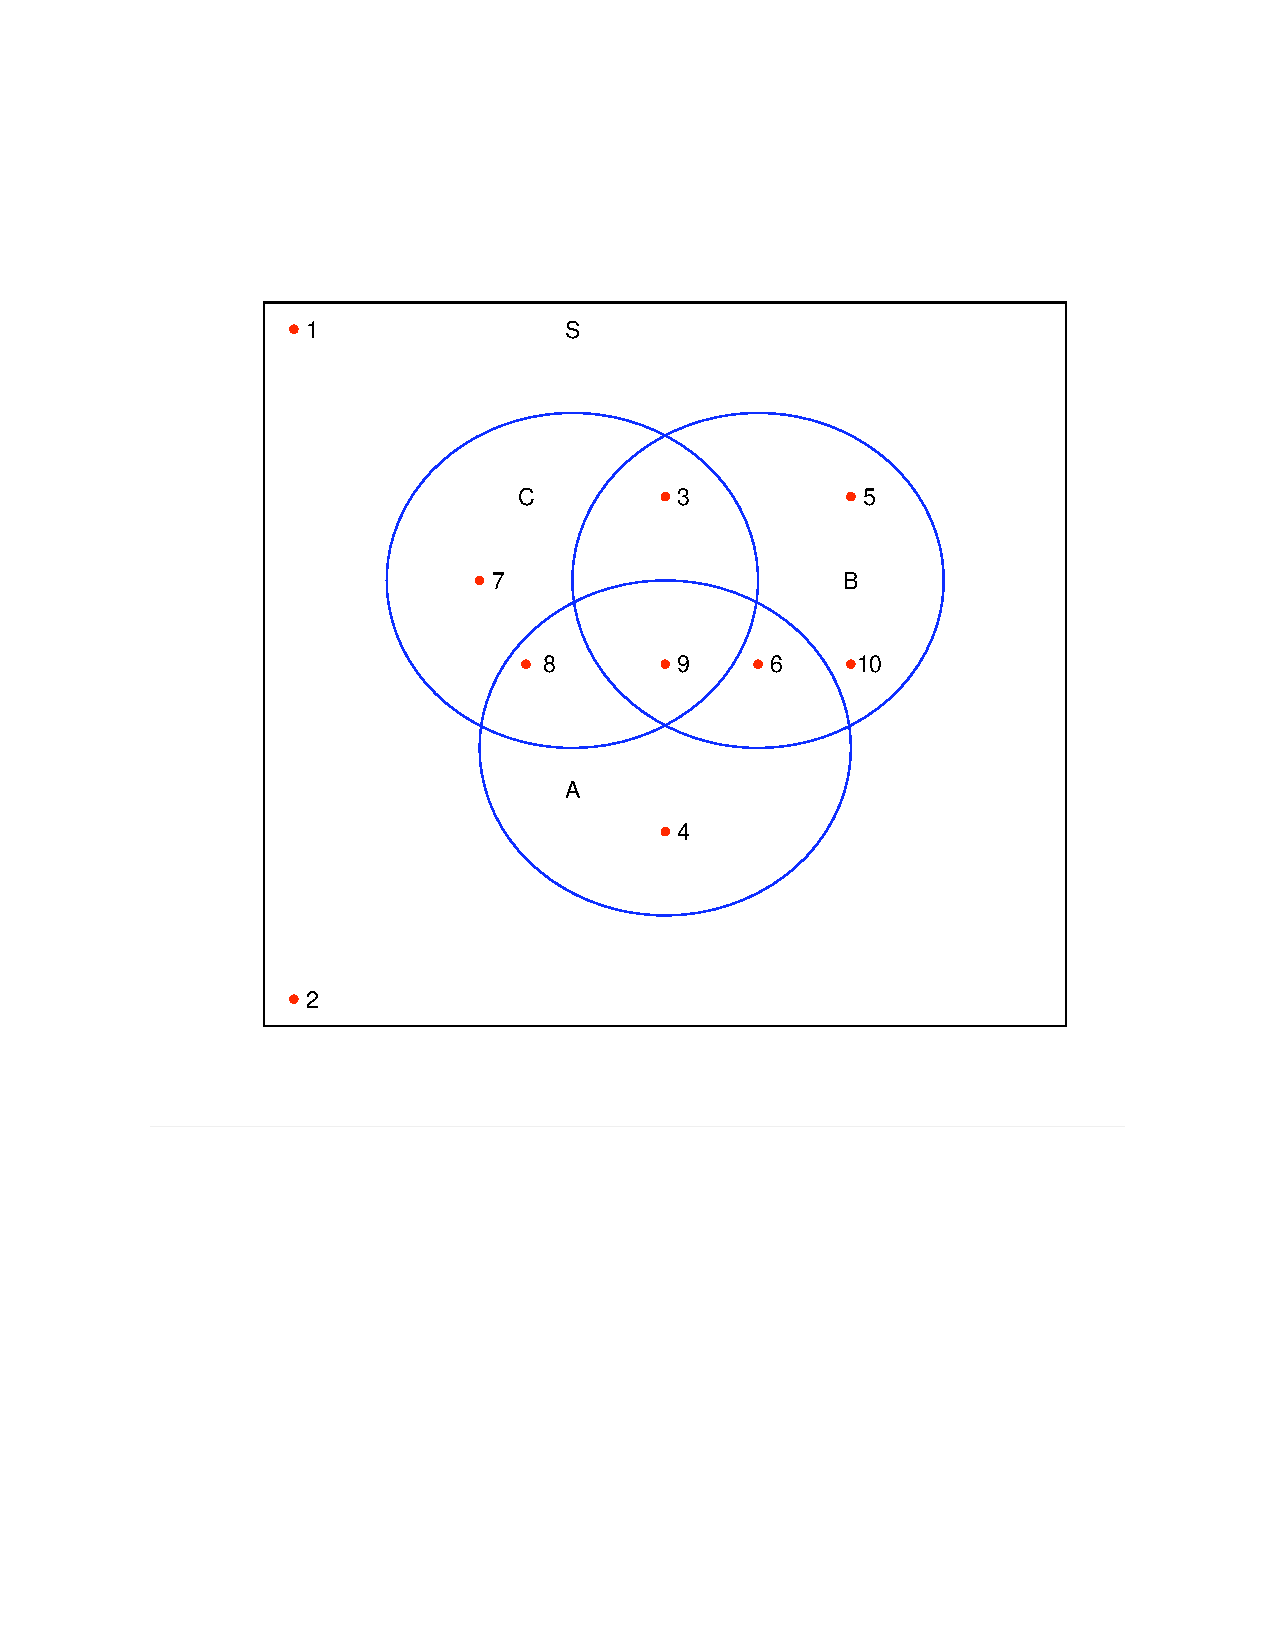
\includegraphics[height=12cm]{a2-fig-2}
\iffalse
\label{se1} \markright{\ref{se1}
\titleref{se1}}
For the following exercises, let\\ $A=[1\ 2],\ B=\left[
\begin{array}{c}3\\2 \end{array}\right ],\ C=\left [\begin
{array}{rr} 1&-2\\2&-3\end {array} \right ],\ D=\left [\begin
{array}{rr} -2&-5\\1&3\end {array} \right ],\\ E=\left [\begin
{array}{rr} 1&5\\3&8
\\2&1\end {array}\right ],\
F=\left [\begin {array}{rrr} 2&-4&1\\6&-9&1\\4&1&6\\1&7&-5\end {array}\right],\
G=\left [\begin {array}{rrr} 1&2&6\\2&-3&7
\\4&-1&3\end {array}\right ],\\
H=\left [\begin {array}{rrr} 1&0&0\\0&1&0
\\-1&0&0\end {array}\right ],\
I=\left [\begin {array}{rrr} 1&0&0\\0&1&0
\\0&0&1\end {array}\right ],\
K=\left [\begin {array}{rrrr} 1&-2&4&7\\2&3&5&-4
\\1&4&2&1\\-2&1&9&4\end {array}
\right ].$
\bigskip

\begin{enumerate}
\item Which of the following operations are not defined? If they
are defined, what is the size of the resulting matrix
\begin{enumerate}
\item $AC$
\item $CA$
\item $KF^t$
\item $KF$
\item $EB+A^t$
\item $E(H+I)$
\end{enumerate}
\item Find: a) $C+D$\quad b) $D+C$ \quad  c) $G+H$ \quad
d) $D-3C$ \quad e) $2D$
\item Find:
\begin{enumerate} \item $AB$ and $BA$
\item $(C+2D)+BA$ and $C+(2D+BA)$
\item $DC$, $ED$, $(ED)C$ and $E(DC)$
\item $FH+FG$ and $F(G+H)$
\item $G^t$, $H^t$, $(GH)^t$, $G^tH^t$ and $H^tG^t$.
\end{enumerate}
\item Find: $KF$, $FG$ and $FH$.
\item Find tr($K$), tr($I$) and tr($E$).
\item Find $C^3$ and $H^2$.
\item Find $I-H$  and $(I-H)^2$.
\item If $f(x)=x^{2} +2x+2$, $g(x)=x^{2}-x-1$, find
\begin{enumerate} \item $f(C), {\rm (b)}~f(D), {\rm (c)}~g(C), {\rm (d)}~g(D)$.
\end{enumerate}
\item Show that if two $n \times n$ matrices $L$, $M$ are symmetric, then so are $L+M$ and $kL$.

\end{enumerate}



\iffalse
\section{Maple Exercises (optional)}

As in the previous session, first open the linear algebra package.

\begin{maplegroup}
\begin{mapleinput}
\mapleinline{active}{1d}{with(linalg):}{%
}
\end{mapleinput}

\end{maplegroup}
\bigskip

In this chapter, matrix operations and the matrix form of a linear
system ( $A{\bf x}={\bf b}$) were introduced.

We will begin this session by giving a second command to construct
a matrix (the first command was given during the previous Maple
session).

\bigskip

\begin{maplegroup}
\begin{mapleinput}
\mapleinline{active}{1d}{A := matrix(3,3, [1,2,3,2,3,4,3,4,5]);}{%
}
\end{mapleinput}

\mapleresult
\begin{maplelatex}
\[
A :=  \left[ {\begin{array}{rrr} 1 & 2 & 3 \\ 2 & 3 & 4 \\ 3 & 4 &
5
\end{array}}
 \right]
\]
\end{maplelatex}

\end{maplegroup}
\begin{maplegroup}
\begin{mapleinput}
\mapleinline{active}{1d}{B:=matrix(3,3,[2,5,7,13,3,5,6,7,8]);}{%
}
\end{mapleinput}

\mapleresult
\begin{maplelatex}
\[
B :=  \left[ {\begin{array}{rrr} 2 & 5 & 7 \\ 13 & 3 & 5 \\ 6 & 7
& 8
\end{array}}
 \right]
\]
\end{maplelatex}

\end{maplegroup}
\begin{maplegroup}
\begin{mapleinput}
\mapleinline{active}{1d}{C:=matrix(4,3,[1,3,5,7,9,0,8,6,4,2,1,7]);}{%
}
\end{mapleinput}

\mapleresult
\begin{maplelatex}
\[
C :=  \left[ {\begin{array}{rrr} 1 & 3 & 5 \\ 7 & 9 & 0 \\ 8 & 6 &
4 \\ 2 & 1 & 7
\end{array}}
 \right]
\]
\end{maplelatex}

\end{maplegroup}
\begin{maplegroup}
\begin{mapleinput}
\mapleinline{active}{1d}{E:=matrix(3,4,[3,4,7,6,9,2,8,2,6,8,3,12]);}{%
}
\end{mapleinput}

\mapleresult
\begin{maplelatex}
\[
E :=  \left[ {\begin{array}{rrrr} 3 & 4 & 7 & 6 \\ 9 & 2 & 8 & 2
\\ 6 & 8 & 3 & 12
\end{array}}
 \right]
\]
\end{maplelatex}

\end{maplegroup}
\bigskip

{\bf Note:} You can not let a matrix be $D$, a Maple error will
result.

Now that we have a few matrices at hand, we will perform some
matrix operations on them. First, scalar multiplication and matrix
addition. These operations are accomplished using the commands:
scalarmul(\emph{matrix name}, \emph{scalar value}) and
matadd(\emph{matrix name},\emph{matrix name}).

\bigskip

\begin{maplegroup}
\begin{mapleinput}
\mapleinline{active}{1d}{scalarmul(B,2);}{%
}
\end{mapleinput}

\mapleresult
\begin{maplelatex}
\[
 \left[
{\begin{array}{rrr} 4 & 10 & 14 \\ 26 & 6 & 10 \\ 12 & 14 & 16
\end{array}}
 \right]
\]
\end{maplelatex}

\end{maplegroup}
\begin{maplegroup}
\begin{mapleinput}
\mapleinline{active}{1d}{matadd(A , B);}{%
}
\end{mapleinput}

\mapleresult
\begin{maplelatex}
\[
 \left[
{\begin{array}{rrr} 3 & 7 & 10 \\ 15 & 6 & 9 \\ 9 & 11 & 13
\end{array}}
 \right]
\]
\end{maplelatex}

\end{maplegroup}
\bigskip

The `matadd' command can also be used to add scalar multiples of
one matrix to another matrix in the following way.
\bigskip

\begin{maplegroup}
\begin{mapleinput}
\mapleinline{active}{1d}{matadd(3*A,-B);}{%
}
\end{mapleinput}

\mapleresult
\begin{maplelatex}
\[
 \left[
{\begin{array}{rrr} 1 & 1 & 2 \\ -7 & 6 & 7 \\ 3 & 5 & 7
\end{array}}
 \right]
\]
\end{maplelatex}

\end{maplegroup}
\begin{maplegroup}
Matrix multiplication is performed using the `multiply' command.

\end{maplegroup}
\begin{maplegroup}
\begin{mapleinput}
\mapleinline{active}{1d}{multiply(A,B);}{%
}
\end{mapleinput}

\mapleresult
\begin{maplelatex}
\[
 \left[
{\begin{array}{rrr} 46 & 32 & 41 \\ 67 & 47 & 61 \\ 88 & 62 & 81
\end{array}}
 \right]
\]
\end{maplelatex}

\end{maplegroup}
\begin{maplegroup}
\begin{mapleinput}
\mapleinline{active}{1d}{multiply(A,B,E);}{%
}
\end{mapleinput}

\mapleresult
\begin{maplelatex}
\[
 \left[
{\begin{array}{rrrr} 672 & 576 & 701 & 832 \\ 990 & 850 & 1028 &
1228 \\ 1308 & 1124 & 1355 & 1624
\end{array}}
 \right]
\]
\end{maplelatex}

\end{maplegroup}
\bigskip

As shown in the previous section, Maple can be used to solve
systems of equations using the row reduction technique. A second
method uses the `linsolve' command. If we have the system $A{\bf
x}={\bf b}$, this command solves for {\bf x}. This command will be
demonstrated with the matrix $B$ from above, and a row matrix or
vector, $b$.

\bigskip

\begin{maplegroup}
\begin{mapleinput}
\mapleinline{active}{1d}{b:=vector([2,3,6]);}{%
}
\end{mapleinput}

\mapleresult
\begin{maplelatex}
\[
b := [2, \,3, \,6]
\]
\end{maplelatex}

\end{maplegroup}
\begin{maplegroup}
\begin{mapleinput}
\mapleinline{active}{1d}{linsolve(B,b);}{%
}
\end{mapleinput}

\mapleresult
\begin{maplelatex}
\[
 \left[  \! {\displaystyle \frac {29}{119}} , \,{\displaystyle
\frac {260}{119}} , \,{\displaystyle -\frac {160}{119}}  \!
 \right]
\]
\end{maplelatex}

\end{maplegroup}
\bigskip

Try solving the same system using the techniques and commands of
the previous Maple session.

The transpose of a matrix was also defined in this section. On
Maple, the transpose of a matrix is found with the `transpose'
command.
\bigskip

\begin{maplegroup}
\begin{mapleinput}
\mapleinline{active}{1d}{transpose(A);}{%
}
\end{mapleinput}

\mapleresult
\begin{maplelatex}
\[
 \left[
{\begin{array}{rrr} 1 & 2 & 3 \\ 2 & 3 & 4 \\ 3 & 4 & 5
\end{array}}
 \right]
\]
\end{maplelatex}

\end{maplegroup}
\begin{maplegroup}
\mapleresult
\begin{maplettyout}
\end{maplettyout}

\end{maplegroup}
\bigskip

Again you might want to try some other examples for yourself.  You
can also combine the commands to simplify long strings of
calculations. \fi

\section{Answers to activity questions and suggested exercises}
\label{answers2}

{\bf Activity questions}

\bigskip

\noindent {\bf \ref{ssec.arith}:} \quad 1.Yes.

\bigskip

\noindent{\bf \ref{ssec.propma}:} \quad Yes.

\bigskip


\noindent{\bf Suggested exercises}

\begin{enumerate}
\item \begin{enumerate}
\item $1 \times 2$
\item undefined
\item undefined
\item $4 \times 3$
\item undefined
\item undefined \end{enumerate}
\item a) $\left [\begin {array}{rr} -1&-7\\3&0\end {array}
\right ]$
b) $\left [\begin {array}{rr} -1&-7\\3&0\end {array}
\right ]$
c) $\left [\begin {array}{rrr} 2&2&6\\2&-2&7
\\3&-1&3\end {array}\right ]$
\\
d) $\left [\begin {array}{rr} -5&1\\-5&12\end {array} \right ]$ e)
$\left [\begin {array}{rr} -4&-10\\2&6\end {array} \right ]$
\item  \begin{enumerate} \item $7$, $\quad \left [\begin {array}{rr} 3&6\\2&4\end {array} \right ]$
\item $\left [\begin {array}{rr} 0&-6\\6&7\end {array}
\right ]$
\item  $\left [\begin {array}{rrr} -12&19\\7&-11\end {array}
\right ]$,  $\left [\begin {array}{rrr} 3&10\\2&9
\\-3&-7\end {array}\right ]$,  $\left [\begin {array}{rr} 23&-36\\20&-31
\\-17&27\end {array}\right ]$,  $\left [\begin {array}{rr} 23&-36\\20&-31
\\-17&27\end {array}\right ]$
\item $\left [\begin {array}{rrr} -1&11&-13\\-3&29&-24
\\28&0&49\\1&-7&40\end {array}
\right ]$, \quad $\left [\begin {array}{rrr} -1&11&-13\\-3&29&-24
\\28&0&49\\1&-7&40\end {array}
\right ]$
\item $G^t=\left [\begin {array}{rrr} 1&2&4\\2&-3&-1
\\6&7&3\end {array}\right ]$, \quad $H^t=\left [\begin {array}{rrr} 1&0&-1\\0&1&0
\\0&0&0\end {array}\right ]$, \\$(GH)^t=\left [\begin {array}{rrr} -5&-5&1\\2&-3&-1
\\0&0&0\end {array}\right ]$ \\

$G^tH^t=\left [\begin {array}{rrr} 1&2&-1\\2&-3&-2
\\6&7&-6\end {array}\right ]$, \quad $H^tG^t=\left [\begin {array}{rrr} -5&-5&1\\2&-3&-1
\\0&0&0\end {array}\right ]$
\end{enumerate}
\item $KF=\left [\begin {array}{rrr} 13&67&-12\\38&-58&55
\\35&-31&12\\42&36&33\end {array}
\right ]$, \quad  $FG=\left [\begin {array}{rrr}
-2&15&-13\\-8&38&-24
\\30&-1&49\\-5&-14&40\end {array}
\right ]$, \\ $FH=\left [\begin {array}{rrr} 1&-4&0\\5&-9&0
\\-2&1&0\\6&7&0\end {array}\right
]$
\item $10$, $3$, $E$ is not square
\item $C^3=\left [\begin {array}{rr} 5&-6\\6&-7\end {array}
\right ]$,\quad $H^2=\left [\begin {array}{rrr} 1&0&0\\0&1&0
\\-1&0&0\end {array}\right ]$
\item $\left [\begin {array}{rrr} 0&0&0\\0&0&0
\\1&0&1\end {array}\right ]$

\item a) $\left [\begin {array}{rr} 1&0\\0&1\end {array} \right ]$
b) $\left [\begin {array}{rr} -3&-15\\3&12\end {array} \right ]$
c) $\left [\begin {array}{rr} -5&6\\-6&7
\\\end {array}\right ]$
d) $\left [\begin {array}{rr} 0&0\\0&0\end {array} \right ]$

\item $(L+M)^{t}=L^{t}+M^{t}=L+M$, $(kL)^{t}=kL^{t}=kL$.
\end{enumerate}

%\end{document}
\fi 
%\iffalse
%\subsection{Exercises}
%
%\begin{frame} \frametitle{Exercises}%\pause
%
%\noindent 11th edition, p. 329,  6.8; p. 334, 6.19 -- 6.21.
%
%\bigskip
%
%\noindent 10th edition, p. 357,  6.17--6.20.
%
%\end{frame}
%\fi
%
%\section{Large Sample Test for a Single Proportion}
%
%\subsection{Large Sample Test for a Single Proportion}
%
%%\frame{ \frametitle{Hypothesis Test for a Single Proportion}%\pause
%
%%\vspace{-1.5 cm}
%
%For a given population proportion $p$ we want to formulate a null hypothesis with respect to
%some fixed level, thus
%\[H_0:  \ p = p_0.\]
%Then we can have,
%
%\begin{itemize}
%  \item[1.] A \textbf{one tailed, upper test} where $H_a$ says $p > p_0$.
%  \item[2.] A \textbf{one tailed, lower test} where $H_a$ says $p < p_0$.
%  \item[3.] A \textbf{two tailed test} where $H_a$ says $p \neq p_0$.
%\end{itemize}
%\iffalse
%\PutAt<1-1>{(2cm,7cm)}{\NormalBox{\parbox[position]{8cm}{\begin{center}\Huge{\alert{$p > p_0$}}\end{center}}}}
%\PutAt<2-2>{(2cm,7cm)}{\NormalBox{\parbox[position]{8cm}{\begin{center}\Huge{\alert{$p > p_0$}}\end{center}}}}
%\PutAt<3-3>{(2cm,7cm)}{\NormalBox{\parbox[position]{8cm}{\begin{center}\Huge{\alert{$p \neq p_0$}}\end{center}}}}
%
%}
%\fi
%\subsection{Test Statistic}
%
%%\frame{ \frametitle{Test Statistic}%\pause
%
%%\vspace{-2 cm}
%
%Let $x_1,\ldots , x_n$ be a random sample from a binomial population that has unknown $p$.  Compute
%\begin{itemize}
%  \item[1.] the sample proportion
%  \item[2.] the sample error, where $q_0=1-p_0$
%  \item[3.] test statistic and suppose $np_0 \geq 15$ and $nq_0 \geq 15$
%\end{itemize}
%\iffalse
%\PutAt<1-1>{(2cm,6cm)}{\NormalBox{\parbox[position]{8cm}{\begin{center}\Huge{$\hat{p}=\frac1n \sum x_i$}\end{center}}}}
%\PutAt<2-2>{(2cm,6cm)}{\NormalBox{\parbox[position]{10cm}{\begin{center}\Huge{
%$\sigma_{\hat{p}}=\sqrt{\frac{p_0q_0}{n}}$}\end{center}}}}
%\PutAt<3-3>{(2cm,6cm)}{\NormalBox{\parbox[position]{8cm}{\begin{center}\Huge{$z= \frac{\hat{p}-p_0}{\sigma_{\hat{p}}}$}\end{center}}}}
%
%
%}
%\fi
%\subsection{Rejection Region}
%
%%\frame{ \frametitle{Rejection Region - One Tailed Test}%\pause
%
%%\vspace{-2 cm}
%
%Fix $\alpha > 0$ (usually $\alpha = 0.05$) so that
%\[P\left(z > z_\alpha \right) = P\left(z <  -z_\alpha \right) = \alpha \]
%where $z$ denotes a standard normal random variable:
%\begin{itemize}
%  \item[1.] one tailed upper test, reject $H_0:  \ p = p_0$ if
%  \item[2.] one tailed lower test, reject $H_0:  \ p = p_0$ if
%\end{itemize}
%\iffalse
%\PutAt<1-1>{(2cm,6cm)}{\NormalBox{\parbox[position]{8cm}{\begin{center}\Huge{$z= \frac{\hat{p}-p_0}{\sigma_{\hat{p}}} > z_\alpha$}\end{center}}}}
%\PutAt<2-2>{(1cm,6cm)}{\NormalBox{\parbox[position]{10cm}{\begin{center}\Huge{$z= \frac{\hat{p}-p_0}{\sigma_{\hat{p}}} < -z_\alpha$}\end{center}}}}
%
%
%
%}
%\fi
%\subsection{Rejection Region}
%
%%\frame{ \frametitle{Rejection Region - Two Tailed Test}%\pause
%
%%\vspace{-2 cm}
%
%Fix $\alpha > 0$ (usually $\alpha = 0.05$) so that
%\[P\left(z > z_{\alpha/2} \right) = P\left(z <  -z_{\alpha/2} \right) = \alpha/2 \]
%where $z$ denotes a standard normal random variable:
%\begin{itemize}
%  \item[1.] two tailed test, reject $H_0:  \ \mu = \mu_0$ if
%  \item[2.] two tailed test, reject $H_0:  \ p = p_0$ if
%\end{itemize}
%
%%\PutAt<1-1>{(2cm,6cm)}{\NormalBox{\parbox[position]{8cm}{\begin{center}\Huge{$z= \frac{\bar{x}-\mu_0}{s/\sqrt{n}} > z_\alpha/2$}\end{center}}}}
%%\PutAt<2-2>{(2cm,6cm)}{\NormalBox{\parbox[position]{10cm}{\begin{center}\Huge{$z= \frac{\bar{x}-\mu_0}{s/\sqrt{n}} < -z_\alpha/2$}\end{center}}}}
%%\PutAt<2-2>{(1cm,6cm)}{\NormalBox{\parbox[position]{10cm}{\begin{center}\Huge{$|z|= \left|\frac{\hat{p}-p_0}{\sigma_{\hat{p}}}\right| > z_{\alpha/2}$}\end{center}}}}
%
%
%
%%}
%
%\subsection{Interpretation}
%
%%\frame{ \frametitle{Test Statistic Falls in Rejection Region}%\pause
%
%%\vspace{-2 cm}
%
%\begin{itemize}
%  \item[1.] we reject the null hypothesis;
%  \item[2.] conclude that the alternative is true;
%  \item[3.] and quantify that we are making this conclusion with the possibility of
%  making a 100$\alpha$\% probability of error (Type I error).
%\end{itemize}
%\iffalse
%\PutAt<1-1>{(2cm,6cm)}{\NormalBox{\parbox[position]{8cm}{\begin{center}\Huge{\alert{REJECT $H_0$}}\end{center}}}}
%\PutAt<2-2>{(2cm,6cm)}{\NormalBox{\parbox[position]{8cm}{\begin{center}\Huge{\alert{ACCEPT $H_a$}}\end{center}}}}
%\PutAt<3-3>{(2cm,6cm)}{\NormalBox{\parbox[position]{8cm}{\begin{center}\Huge{\alert{100$\alpha$\% ERROR}}\end{center}}}}
%
%}
%\fi
%%________________________________________________________________________
%
%%\subsection{Interpretation}
%
%%\frame{ \frametitle{Test Statistic Does Not Fall in Rejection Region}%\pause
%
%%\vspace{-2 cm}
%
%\begin{itemize}
%  \item[1.] we do not reject the null hypothesis;
%  \item[2.] we do not conclude that the null hypothesis is true;
%  \item[3.] because in general we do not know the probability $\beta$ of incorrectly accepting $H_0$ (Type II error).
%\end{itemize}
%\iffalse
%\PutAt<1-1>{(2cm,6cm)}{\NormalBox{\parbox[position]{8cm}{\begin{center}\Huge{\alert{DO NOT REJECT $H_0$}}\end{center}}}}
%\PutAt<2-2>{(2cm,6cm)}{\NormalBox{\parbox[position]{8cm}{\begin{center}\Huge{\alert{RESERVE JUDGEMENT ON $H_0$}}\end{center}}}}
%\PutAt<3-3>{(2cm,6cm)}{\NormalBox{\parbox[position]{8cm}{\begin{center}\Huge{\alert{DO NOT KNOW $\beta$}}\end{center}}}}
%
%}
%\fi
%\subsection{Examples}
%
%%\begin{frame} \frametitle{Examples}%\pause
%
%Will be discussed in class.
%
%%\end{frame}
%

\subsection{Exercises}
\begin{enumerate}
\item For two events,$A$ and $B$,$P(A)=0.3$,$P(B)=0.2$,and$P(A\bigcap B)=0.1$.

\begin{enumerate}
\item Find $P(A\bigcup B)$.
\item Find $P(A|B)$.
\item Find $P(B|A)$.
\item Are $A$ and $B$ independent events?Justify your answer. 
\end{enumerate}
\item For two events,$A$ and $B$,$P(A)=0.4$,$P(B)=0.3$,and$P(A|B)=0.6$.

\begin{enumerate}
\item Find$P(A\bigcap B)$.
\item Find $P((B|A)$.
\end{enumerate}

\item For two independent events,$A$ and $B$,$P(A)=0.4$,$P(B)=0.3$.
\begin{enumerate}
\item Find $P(A\bigcup B)$.
\item Find $P(A|B)$.
\item Find $P(B|A)$.
\end{enumerate}



\item For two mutually exclusive events,$A$ and $B$,$P(A)=0.3$,$P(B)=0.7$.Find each of the following probabilities:
\begin{enumerate}
\item List the sample points for this experiment.
\item Find $P(A\bigcap B)$.
\item Find $P(B|A)$.
\item Find $P(A\bigcup B)$.
\end{enumerate}
%\item Show that if two $n \times n$ matrices $L$, $M$ are symmetric, then so are $L+M$ and $kL$.

\end{enumerate}



\iffalse
\begin{frame} \frametitle{Exercises}%\pause

\noindent Exercises:

\bigskip

\noindent 11th edition, p. 151:  3.47-3.51

\bigskip

\noindent 10th edition, p. 166:  3.41-3.45

\end{frame}
\fi 
%\section{Summary}\label{ssec.sumry2}
%\markright{\ref{ssec.sumry2} \titleref{ssec.sumry2}}
%{\bf Section Keywords: hypothesis;null hypothesis.alternative hypothesis;
%test statistic;rejection region;Type I error;size;significance level;
%false positive;Type II error;$\beta$;false negative;
%one tailed, upper test;one tailed, lower test;
%two tailed test;
%}
%
%
%\iffalse
%In this short chapter, we leave the study of linear systems to define
%eigenvalues and eigenvectors. It is beyond the scope of the course
%to discuss all the practical applications of this topic. However,
%it is a topic important to many different areas, including the
%solution and study of differential equations. An application will
%be given in the next chapter.
%
%\noindent {\bf Learning Objectives}
%
%\noindent After completing this chapter, you should be able to:
%\begin{itemize}
%\item define what is meant by an eigenvalue and an eigenvector
%\item find the characteristic polynomial
%\item determine the eigenvalues and eigenvectors of a matrix
%\item find the basis for an eigenspace
%\item find the limiting probabilities of a Markov chain
%\item diagonalize a matrix.
%\end{itemize}
%
%\section{Eigenvalues, Eigenvectors and Eigenspaces}
%\label{ssec.edef} \markright{\ref{ssec.edef} \titleref{ssec.edef}}
%
%The notion of eigenvalues and eigenvectors is of fundamental
%importance in matrix algebra, and has applications throughout
%mathematics and the sciences.  In this chapter we study eigenvalues
%and eigenvectors.  We give two simple applications in chapter 8, but
%many applications remain beyond the scope of this course.
%
%Let $A$ be an $n\times n$ matrix.  A vector ${\bf x}\in \mbox{\tebbb R}^n$ is an
%{\bf eigenvector}\index{eigenvector} for $A$ if
%\begin{enumerate}
%\item
%${\bf x}\neq{\bf 0},$
%\item
%$A{\bf x}=\lambda{\bf x}$ for some scalar $\lambda$.
%\end{enumerate}
%
%The scalar $\lambda$ is called the {\bf eigenvalue}\index{eigenvalue} of $A$ corresponding to
%the eigenvector {\bf x}.  Likewise we say that {\bf x} is an eigenvector
%corresponding to $\lambda$.
%
%You may wonder why the definition precludes {\bf 0} from
%being an eigenvector.  The reason is that if we allowed {\bf 0}
%to be an eigenvector then
%$$A\cdot{\bf 0}={\bf 0}=\lambda{\bf 0}\ {\rm for}\ {\rm all}\ {\rm scalars}\  \lambda.$$
%This would mean that {\bf every} scalar $\lambda$ is an eigenvalue and
%we want to avoid this.
%
%If $\lambda$ is an eigenvalue of $A$, the set
%$$V_\lambda=\{{\bf x}\in \mbox{\tebbb R}^n:A{\bf x}=\lambda{\bf x}\}$$
%is called the {\bf eigenspace}\index{eigenspace} of $A$ corresponding to $\lambda$ (or sometimes
%just the {\bf eigenspace for $\lambda$}).  This set is a vector subspace of
%$\mbox{\tebbb R}^n$ because,
%\begin{enumerate}
%\item
%$A{\bf 0}={\bf 0}=\lambda{\bf 0}$ means that ${\bf 0}\in V_\lambda$.
%\item
%If ${\bf x_1},\ {\bf x_2} \in V_\lambda$, then $A{\bf x_1}=\lambda{\bf x_1},
%\ A{\bf x_2}=\lambda{\bf x_2}.$  Therefore
%$A({\bf x_1}+{\bf x_2})=A{\bf x_1}+A{\bf x_2}=\lambda{\bf x_1}+\lambda{\bf x_2}
%=\lambda({\bf x_1}+{\bf x_2})$ and $({\bf x_1}+{\bf x_2}) \in  V_\lambda.$
%\item
%If ${\bf x}  \in  V_\lambda$ (so that $A{\bf x}=\lambda{\bf x}$) and
%c is a scalar, then
%$A(c{\bf x})=cA{\bf x}=c\lambda{\bf x}=\lambda(c{\bf x}).$  This means
%that $c{\bf x} \in  V_\lambda.$
%\end{enumerate}
%
%The eigenspace of $A$ corresponding to $\lambda$ consists of all
%the eigenvectors of $A$ corresponding to $\lambda$, together with the zero
%vector.  As noted above, the zero vector is not an eigenvector by
%definition.
%
%Note that the scalar zero can be an eigenvalue.
%In fact when $\lambda=0$ is an eigenvalue for $A$, the corresponding
%eigenspace is the set \{{\bf x}\ :\ A{\bf x}={\bf 0}\}. We recognize this as the
%nullspace of $A$.
%
%%In this section, we give the mathematical definition for an
%%eigenvalue and an eigenvector of a matrix.
%
%In $\mbox{\tebbb R}^2$ and $\mbox{\tebbb R}^3$ there is a geometric
%interpretation for eigenvectors and eigenvalues.  If we take a vector
%{\bf x} and multiply it
%by the matrix $A$ then the result (A{\bf x}) is a vector that could point in
%any direction.  When {\bf x} is an eigenvector for $A$, $A{\bf x}=\lambda{\bf x}$
%and so
%$A{\bf x}$ points along the same line as ${\bf x}$.
%\begin{enumerate}
%\item
%$\lambda\ >\ 0$
%\begin{center}
%\begin{picture}(90,90)(-20,-20)
%\put(-10,-10){\vector(4,3){30}} \put(10,-2){\bf x}
%\put(40,40){$A{\bf x}$} \put(-10,-10){\vector(4,3){70}}
%\end{picture}
%\end{center}
%\item
%$\lambda\ <\ 0$
%\begin{center}
%\begin{picture}(90,90)(-20,-20)
%\put(-10,-10){\vector(4,3){70}}
%\put(5,-9){$A{\bf x}$}
%\put(40,40){\bf x} \put(-10,-10){\vector(-4,-3){20}}
%%\put(1,0.8){$\circ$}
%\end{picture}
%\end{center}
%\end{enumerate}
%
%The eigenvalue $\lambda$ gives the scaling factor between ${\bf x}$
%and $A{\bf x}$.  If $\lambda$
%is positive then $A{\bf x}$ points in the same direction as ${\bf x}$.
%If $\lambda$ is
%negative then $A{\bf x}$ points in the opposite direction to ${\bf x}$.
%
%\begin{example}
%\label{exam9.evalue}
%Let $$A=\left [ \begin{array}{rr} 1&4\\
%                              3&2 \end{array} \right ],
%\quad
%                {\bf x}=\left [ \begin{array}{r} 1\\ 1 \end{array} \right
%                ].$$
%
%$$A{\bf x}= \left [ \begin{array}{rr}
%                                1&4\\
%                                3&2 \end{array} \right ]
%                                \left [ \begin{array}{r} 1\\ 1 \end{array} \right]
%= \left [\begin{array}{r} 5\\ 5 \end{array} \right ] = 5\left[
%\begin{array}{r} 1\\ 1 \end{array} \right ].$$
%Therefore, $\lambda=5$ is an eigenvalue of $A$ and ${\bf x}=\left[
%\begin{array}{r} 1\\ 1 \end{array} \right ]$ is an eigenvector.
%The eigenspace for $\lambda=5$ is obtained by solving
%\begin{eqnarray*}
%\left [ \begin{array}{rr}
%      1&4\\
%      3&2 \end{array} \right ]
%\left [ \begin{array}{r} x_1\\ x_2 \end{array} \right ] &=&5\left
%[ \begin{array}{r} x_1 \\ x_2 \end{array} \right ],
%\end{eqnarray*}
%i.e.
%\begin{eqnarray*}
%x_1+4x_2&=&5x_1 \\
%3x_1+2x_2&=&5x_2, \end{eqnarray*}
%\begin{eqnarray*}
%or~\left [ \begin{array}{rr}
%      -4&4\\
%      3&-3 \end{array} \right ]
%\left [ \begin{array}{r} x_1\\ x_2 \end{array} \right ] &=& \left[
%\begin{array}{r} 0 \\ 0 \end{array} \right ].
%\end{eqnarray*}
%By row reduction,
%$$\left [ \begin{array}{rrcr} -4&4& \vline& 0 \\
%3&-3&\vline&0 \end{array} \right
%] \leadsto \left [ \begin{array}{rrcr} 1&-1& \vline&0 \\
%0&0&\vline&0 \end{array} \right ].$$ Let $x_2=s$, then $x_1=s$ and
%the solution space is $\{s(1,1):s~\epsilon \mbox ~{\tebbb R}\}$.
%Not only is $\left[ \begin {array}{r}1 \\1 \end{array} \right]$ an
%eigenvector for $\lambda=5$, but any non-zero multiple of $\left[ \begin
%{array}{r}1 \\1 \end{array} \right]$ is also an eigenvector. The
%eigenspace for $\lambda=5$ is a line through the origin.
%\end{example}
%
%\begin{example}
%\label{exam9.evalue2}
%Let $$A=\left[\begin {array}{rrr} 0&0&3\\5&1&2\\2&0&1\end{array}\right].$$
%Given that $\lambda=3$ is an
%eigenvalue for $A$, find an eigenvector corresponding to $\lambda=3$, and
%the eigenspace corresponding to $\lambda=3$.
%
%To find an eigenvector for $\lambda=3$ we must find
%$\left[\begin{array}{r}x_1\\x_2\\x_3\end{array}\right]\neq
%\left[\begin{array}{r}0\\0\\0\end{array}\right]$
%such that
%$$\left[\begin{array}{rrr}0&0&3\\5&1&2\\2&0&1\end{array}\right]
%\left[\begin{array}{r}x_1\\x_2\\x_3\end{array}\right]=
%3\left[\begin{array}{r}x_1\\x_2\\x_3\end{array}\right],$$
%i.e.
%\begin{eqnarray*}
%3x_3=3x_1\\
%5x_1+x_2+2x_3=3x_2\\
%2x_1+x_3=3x_3,
%\end{eqnarray*}
%or
%\begin{eqnarray*}
%3x_1-3x_3=0\\
%5x_1-2x_2+2x_3=0\\
%-2x_1+2x_3=0.
%\end{eqnarray*}
%
%Reducing the system of equations yields
%$$\left[\begin{array}{rrrcr}3&0&-3&\vline&0\\
%5&-2&2&\vline&0\\
%-2&0&2&\vline&0\end{array}\right]\rightarrow
%\left[\begin{array}{rrrcr}1&0&-1&\vline&0\\
%0&1&-\frac{7}{2}&\vline&0\\
%0&0&0&\vline&0\end{array}\right]$$
%
%The solution space is \{s $(1,\frac{7}{2},1)$:s $\in \mbox{\tebbb R}$\} and this
%is the
%eigenspace for $\lambda=3$.  An eigenvector is
%$\left[\begin{array}{r}1\\\frac{7}{2}\\1\end{array}\right],$ or
%$\left[\begin{array}{r}2\\7\\2\end{array}\right],$ or
%$\left[\begin{array}{r}-4\\-14\\-4\end{array}\right],$ etc.
%\end {example}
%
%In \ref {exam9.evalue} an eigenvector was given and we found the
%eigenvalue, while in Example \ref {exam9.evalue2} an eigenvalue was given and
%we found the eigenvectors.  Suppose that neither is given and we
%are just presented with the matrix $A$.  How do we find the
%eigenvalues and eigenvectors?
%
%We need to find ${\bf x}\neq{\bf 0}$ and $\lambda$ such that
%$$A{\bf x}=\lambda{\bf
%x}.$$
%Since multiplying by the identity matrix changes nothing, this is the
%same as
%\begin{equation}\label{eigen1}
%A{\bf x}=\lambda  I
%{\bf x},
%\ \
%{\rm or} \ \
%(\lambda\  I -A){\bf x}={\bf 0}.
%\end{equation}
%
%If $A$ is an $n \times n$ matrix and
%${\bf x}=\left[\begin{array}{c}x_1\\x_2\\\vdots\\x_n\end{array}\right]$
%then (\ref{eigen1}) is a system of
%$n$ equations in the unknowns $x_1, x_2,\cdots,x_n$ and we require that
%this system of equations has a non-zero solution.  By Theorem \ref{thm6.3}
%a condition for this is that the matrix of coefficients has
%determinant zero:
%\begin{equation}\label{eigen3}
%{\rm det}(\lambda\ I -A)=0 \quad .
%\end{equation}
%${\rm Det}(\lambda\ I -A)$ is a polynomial in $\lambda$, of degree $n$.  It is
%called the
%{\bf characteristic polynomial}\index{characteristic polynomial} of $A$, and (\ref{eigen3}) is called the
%{\bf characteristic equation}\index{characteristic equation}.  The roots of the characteristic polynomial
%give the
%eigenvalues of the matrix $A$.  Once we have found an eigenvalue\index{eigenvalue}
%($\lambda_1$ say), we find the corresponding eigenvectors and eigenspace \index{eigenspace}by
%solving the system $(\lambda_1 I -A){\bf x}={\bf 0}$
%(as we did in Example \ref {exam9.evalue2}).
%\begin{example}
%\label {exam9.evalue3}
%Let $$A=\left[\begin{array}{rr}1&4\\
%3&2\end{array}\right].$$  Then the
%characteristic equation is
%$$det\left[\begin{array}{rr}(\lambda-1)&-4\\-3&(\lambda-2)\end{array}\right]=0.$$
%Evaluating the determinant yields
%$$(\lambda-1)(\lambda-2)-12=\lambda^2-3\lambda-10
%=(\lambda-5)(\lambda+2).$$
%The eigenvalues are therefore $\lambda=-2,\ 5.$
%To find the eigenspace for $\lambda=-2$, we put $\lambda=-2$ in
%$$(\lambda I -A){\bf x}={\bf 0},$$
%and solve for ${\bf x}$:
%$$\left(\left[\begin{array}{rr}-2&0\\0&-2\end{array}\right]-
%\left[\begin{array}{rr}1&4\\3&2\end{array}\right]\right)
%\left[\begin{array}{r}x_1\\x_2\end{array}\right]=
%\left[\begin{array}{r}0\\0\end{array}\right],$$
%i.e.
%$$\left[\begin{array}{rr}-3&-4\\-3&-4\end{array}\right]
%\left[\begin{array}{r}x_1\\x_2\end{array}\right]=
%\left[\begin{array}{r}0\\0\end{array}\right].$$
%Reducing, we find
%$$\left[\begin{array}{rrcr}-3&-4&\vline&0\\-3&-4&\vline&0\end{array}\right]
%\rightarrow
%\left[\begin{array}{rrcr}1&\frac{4}{3}&\vline&0\\0&0&\vline&0\end{array}\right]$$
%The solution is \{s$(-\frac{4}{3},1)$:s $\in \mbox{\tebbb R}$\},
%so this is the eigenspace for
%$\lambda=-2$.  An eigenvector is $\left[\begin{array}{r}-\frac{4}{3}\\
%1\end{array}\right],$ or
%$\left[\begin{array}{r}-4\\3\end{array}\right],$ or
%$\left[\begin{array}{r}4\\-3\end{array}\right],\cdots$
%
%For $\lambda=5$, we must solve
%$$\left(\left[\begin{array}{rr}5&0\\0&5\end{array}\right]-
%\left[\begin{array}{rr}1&4\\3&2\end{array}\right]\right)
%\left[\begin{array}{r}x_1\\x_2\end{array}\right]=
%\left[\begin{array}{r}0\\0\end{array}\right],$$
%i.e.
%$$\left[\begin{array}{rr}4&-4\\-3&3\end{array}\right]
%\left[\begin{array}{r}x_1\\x_2\end{array}\right]=
%\left[\begin{array}{r}0\\0\end{array}\right].$$
%Reducing yields
%$$\left[\begin{array}{rrcr}4&-4&\vline&0\\-3&3&\vline&0\end{array}\right]
%\rightarrow
%\left[\begin{array}{rrcr}1&-1&\vline&0\\0&0&\vline&0\end{array}\right].$$
%The solution is \{s$(1,1)$:s $\in \mbox{\tebbb R}$\} so this is the
%eigenspace for $\lambda=5$.  An
%eigenvector is $\left[\begin{array}{r}1\\1\end{array}\right],$ or
%$\left[\begin{array}{r}2\\2\end{array}\right],$ or
%$\left[\begin{array}{r}-1\\-1\end{array}\right],\cdots$
%\end {example}
%To summarize: if $A$ is $n\times n$ and $\lambda$ is a scalar then the
%following statements are equivalent:
%\begin{description}
%\item (a) $\lambda$ is an eigenvalue of $A$.
%\item (b) there exists ${\bf x}\neq 0 \in \mbox{\tebbb R}^n$ such that $A{\bf
%x}=\lambda{\bf x}$.
%\item (c) The system $(\lambda \ I -A){\bf x}={\bf 0}$ has a non
%trivial solution.
%\item (d) $\lambda$ is a solution to the characteristic equation
%${\rm det}(\lambda \ I -A)=0$.
%\end{description}
%
%\section{Calculation of Eigenvalues and Eigenvectors}
%\label{ssec.ecal} \markright{\ref{ssec.ecal} \titleref{ssec.ecal}}
%
%We find eigenvalues by finding the roots of the characteristic
%polynomial.  If $A$ is $n\times n$ then the characteristic polynomial has
%degree $n$.  While it is easy to find the roots of a quadratic
%equation (when $n=2$) factorizing polynomials of higher degree is
%difficult without computer assistance.  For $n=3$ the characteristic
%equation is a cubic equation with real coefficients.  Such an equation
%always has at least one real root.  There is a method for finding the
%roots of a cubic equation, but the method is difficult to apply
%and is rarely used.  In this course we will use the Remainder
%Theorem, or rely on properties of the determinant to factorize
%cubic equations (the Remainder Theorem only applies in
%limited circumstances).  A brief discussion of the Remainder
%Theorem is given in subsection \ref{remainder}.
%
%For $n\geq4$ there is no practical method for factorizing
%the characteristic polynomial, so we restrict our attention to
%the $2\times 2$ and the $3\times 3$ case.
%
%\subsubsection{${\bf 2 \times 2}$ Matrices}
%\label{emat2}
%The characteristic polynomial for a $2 \times 2$ matrix,
%$$\left| \begin{array}
%{rr}
%                                \lambda-a_{11}&-a_{12}~ \\
%                                -a_{21}~&\lambda-a_{22} \end{array} \right|$$
%is a quadratic polynomial, whose roots can be found either by
%factorization or by the well-known formula. Once an eigenvalue has
%been obtained it is a simple matter to find the eigenspace as the
%nullspace of $(\lambda I - A)$.
%
%\begin{example}
%\label{exam9.findevalue} Find any eigenvalues of
%$$\left [ \begin{array}{rr}
%    4 & -5 \\
%    2 & -3 \end{array} \right].$$
%The characteristic polynomial is
%\begin{eqnarray*} \left| \begin{array}{cc} \lambda-4 & 5~ \\ -2~ & \lambda+3
%\end{array} \right|&=&(\lambda-4)(\lambda +3)+10 = \lambda^2- \lambda -12+10 \\
%&=&\lambda^2- \lambda -2=(\lambda-2)(\lambda+1).
%\end{eqnarray*}
%
%The eigenvalues are $\lambda_1=2$, $\lambda_2=-1$. The eigenspace
%for $\lambda_1=2$ is the nullspace if the matrix
%$$\left [ \begin{array}{rr}
%    2-4 & 5~~ \\
%    -2~ & 2+3 \end{array} \right]= \left [ \begin{array}{rr}
%    -2 & 5 \\
%    -2 & 5 \end{array} \right].$$
%Reducing the matrix yields
%$$\left [ \begin{array}{rr} -2&5 \\ -2&5 \end{array} \right]
%\leadsto \left [ \begin{array}{rr} 1&-\frac{5}{2} \\
%0&0 \end{array} \right ].$$
%
%Let $x_2=s$, so $x_1=\frac{5s}{2}$ and the eigenspace is $\{
%s\left( \frac{5}{2},1 \right):s~\epsilon~\mbox {\tebbb R} \}$. An
%eigenvector is obtained by choosing a non-zero value for s. Hence
%$\left[ \begin{array}{r} 5/2 \\ 1~ \end{array} \right]$ is an
%eigenvector, as is $\left[ \begin{array}{r} 5 \\ 2 \end{array}
%\right]$.
%
%\noindent The eigenspace for $\lambda_2=-1$ is the nullsapce of
%the matrix
%$$\left [ \begin{array}{rr}
%    -1-4 & 5~~ \\
%    -2~~ & -1+3 \end{array} \right]= \left [ \begin{array}{rr}
%    -5 & 5 \\
%    -2 & 2 \end{array} \right].$$
%This matrix reduces to $\left[ \begin{array}{rr} 1&-1 \\ 0&0
%\end{array} \right]$, and the eigenspace is $\{ s \left( 1,
%1 \right):s~\epsilon~\mbox {\tebbb R} \}$. An eigenvector is
%$\left[ \begin{array}{r} 1 \\ 1 \end{array} \right]$, or $\left[
%\begin{array}{r} 2 \\ 2 \end{array} \right]$ etc.
%\end{example}
%
%Three important points to note
%\begin{itemize}
%\item If {\bf x} is an eigenvector for $A$ with eigenvalue
%$\lambda$, then so is any non-zero multiple of {\bf x}, (c{\bf x},
%$c\neq 0)$.
%\item If $\lambda_1$ is an eigenvalue of $A$, then the matrix
%$(\lambda_1 I - A)$ must have nullity $\geq1$.  This means
%that when you reduce
%$(\lambda_1 I - A)$ you must get at least one row of zeros.  If you
%don't then you have made a mistake.
%\item It is easy to check your answers.  If you think $\lambda_1$ is
%an eigenvalue for $A$ with eigenvector ${\bf x_1}$, then multiply out
%$A{\bf x_1}$.  If this equals $\lambda_1{\bf x_1}$ then you are right.
%If it doesn't
%equal $\lambda_1{\bf x_1}$ then you are wrong.
%\end{itemize}
%
%\begin{example}
%\label{exam9.noevalue} Find any eigenvalues and eigenvectors of
%$$A=\left [
%\begin{array}{rr} -1&-5 \\ 1&1  \end{array} \right ].$$
%The characteristic polynomial is
%$$\left| \begin{array}{cc}
%\lambda+1&5 \\ -1&\lambda-1  \end{array} \right|
%=(\lambda+1)(\lambda-1)+5=\lambda^2+4.$$ The roots of this
%polynomial are $\frac{-0\pm \sqrt{0^2-4 \cdot4}}{2}=\pm
%\sqrt{-4}=\pm 2i$, where i is the imaginary number satisfying
%$i^2=-1$. Eigenvectors can be found in the usual way, but some
%complex arithmetic is required. For $ \lambda_1=2i$, the eigenspace
%is the nullspace of $\left [ \begin{array}{rr} 2i+1&5~~
%\\ -1~~&2i-1
%\end{array} \right ]$.
%
%This reduces to $\left [\begin{array}{rr} 1&(1-2i) \\ 0&0
%\end{array} \right ]$, so an eigenvector for $\lambda_1=2i$ is $\left [
%\begin{array}{r} 2i-1 \\ 1~~ \end{array} \right ]$. Similarly for
%$\lambda_2=-2i$, we require the nullspace of $\left [
%\begin{array}{rr} -2i+1&5~~ \\ -1~~&-2i-1  \end{array} \right ]$,
%which reduces to $\left[ \begin{array}{rr} 1&2i+1 \\ 0&0~~
%\end{array} \right ]$. An eigenvector for $\lambda_2=-2i$ is $\left [
%\begin{array}{r} 2i+1 \\ -1~ \end{array} \right ]$.
%\end{example}
%
%Notice that a matrix with real entries can have eigenvalues and
%eigenvectors that are complex.
%
%\subsubsection{${\bf 3\times 3}$ Matrices}
%\label{emat3}
%
%The characteristic polynomial for a $3\times 3$ matrix A is
%$$\det(\lambda I-A)=\left|
%\begin{array}{rrr} \lambda-a_{11}&-a_{12}~~&-a_{13}~~ \\
%-a_{21}~~&\lambda-a_{22}&-a_{23}~~ \\
%-a_{31}~~&-a_{32}~~&\lambda-a_{33}
%\end{array} \right|=0.$$ It is a cubic polynomial, the roots of which
%are the eigenvalues of A. Even though a cubic polynomial with real
%coefficients always has at least one real root, there is no simple
%method that guarantees finding the roots. There are two ways of
%proceeding that are illustrated in the following example.
%\begin{example} Find the eigenvalues of $$A=\left [
%\begin{array}{rrr} 0&0&3 \\ 5&1&2 \\ 2&0&1  \end{array} \right ].$$
%
%We have to find the roots of the characteristic polynomial.
%Expanding along the top row yields
%\begin{eqnarray*}\left|
%\begin{array}{rrr} \lambda&0~~&-3~ \\ -5&\lambda-1&-2~
%\\-2&0~~&\lambda-1  \end{array} \right|
%%&=&\lambda \left( (\lambda-1)^2-0(-2) \right) -0 \left(
%%-5(\lambda-1)-(-2)(-2) \right)-3\left( -5\cdot0+2(\lambda-1)
%%\right)
%&=& \lambda^3-2\lambda^2-5\lambda+6.
%\end{eqnarray*}
%The first way of proceeding is to use the Remainder Theorem
%and observe that $\lambda=1$ is a
%root of the polynomial, because $$1^3-2\cdot1^2-5\cdot1+6=0.$$
%This means that $(\lambda-1)$ divides the characteristic
%polynomial. Dividing $(\lambda-1)$ into
%$(\lambda^3-2\lambda^2-5\lambda+6)$ gives $\lambda^2-\lambda-6$.
%This factorizes into $(\lambda-3)(\lambda+2)$. Hence
%$(\lambda^3-2\lambda^2-5\lambda+6)=(\lambda-1)(\lambda-3)(\lambda+2)$
%and the eigenvalues are $1,-2,3$.
%
%The second way of proceeding is to use the properties of
%determinants. In this case we could have observed that
%$(\lambda-1)$ is a factor of every term in the second column, so
%that $$\left|
%\begin{array}{rrr} \lambda&0~~&-3~ \\ -5&\lambda-1&-2~
%\\-2&0~~&\lambda-1  \end{array} \right|=(\lambda-1)\left|
%\begin{array}{rrr} \lambda&0&-3~ \\ -5&1&-2~
%\\-2&0&\lambda-1  \end{array} \right|.$$
%We can now expand down the middle column to obtain
%\begin{eqnarray*}(\lambda-1)\left|
%\begin{array}{rr} \lambda&-3~ \\ -2&\lambda-1  \end{array} \right|
%&=&(\lambda-1)[\lambda(\lambda-1)-6]=(\lambda-1)(\lambda^2-\lambda-6)
%\\ &=& (\lambda-1)(\lambda+2)(\lambda-3).
%\end{eqnarray*}
%Again, we have established that eigenvalues are $1,-2,3$.
%\end{example}
%
%Other properties of determinants can be used to find eigenvalues,
%as the following example demonstrates.
%
%\begin{example} Find the eigenvalues of $$A=\left[
%\begin{array}{rrr} -9&4&4 \\ -8&3&4 \\ -16&8&7  \end{array} \right].$$
%We have to find the roots of the characteristic equation.
%
%\begin{eqnarray*} &&\left|\begin{array}{rrr} \lambda+9&-4~&-4~
%                                        \\ 8~~&\lambda-3&-4~
%                                        \\ 16~&-8~&\lambda-7
%                        \end{array} \right|
%\\
%&=& \left|\begin{array}{rrr} \lambda+1&-4&-4
%                            \\ \lambda+1& \lambda-3&-4
%                            \\ \lambda+1&-8&\lambda-7  \end{array} \right|
%                                                  \quad\quad C_1=C_1+C_2+C_3
%\\
%&=& (\lambda+1)\left| \begin{array}{rrr} 1&-4~&-4~ \\
%                                        1&\lambda-3&-4~ \\
%                                        1&-8~&\lambda-7
%                                        \end{array} \right|
%\\
%&=& (\lambda+1)\left| \begin{array}{rrr} 0&-1-\lambda&0~~ \\
%                                        1&\lambda-3&-4~ \\
%                                        1&-8~&\lambda-7
%                                        \end{array} \right| \quad\quad R_1=R_1-R_2
%\\
%&=&(\lambda+1)^2 \left| \begin{array}{rrr} 0&-1&0~~ \\
%                                        1&\lambda-3&-4~ \\
%                                        1&-8~&\lambda-7
%                                        \end{array} \right|
%\\
%&=&(\lambda+1)^2(\lambda-7+4) \quad\quad (expanding~along~top~row)
%\\
%&=&(\lambda+1)^2(\lambda-3).
%\end{eqnarray*}
%Hence the eigenvalues are $-1,-1,3$.
%\end{example}
%
%Once the eigenvalues have been found, eigenspaces and eigenvectors
%can be found as in the $2\times 2$ case, by finding the nullspace
%of $(\lambda I-A)$.
%
%\begin{example}
%\label{exam9.findbase} Find bases for the eigenspaces of
%$$A=\left[
%\begin{array}{rrr}
%    0&0&-2\\
%    1&2&1\\
%    1&0&3 \end{array} \right ] .$$
%Solve the characteristic equation:
%\begin{eqnarray*}
%0&=&|\lambda I -A|\\ &=&\lambda^3-5\lambda^2+8\lambda -4\\
%&=&(\lambda-1)(\lambda-2)^2 \quad .
%\end{eqnarray*}
%Therefore, $\lambda=1$ and $\lambda=2$ are the eigenvalues of $A$.
%Note that $\lambda=2$ is a repeated eigenvalue.
%
%Find the eigenvectors:
%$\lambda=2$: $$\left [ \begin{array}{rrr}
%                        2&0&2\\
%                        -1&0&-1\\
%                        -1&0&-1 \end{array} \right ] \left [
%                        \begin{array}{c} x_1\\ x_2 \\x_3
%                        \end{array} \right ]=\left [
%                        \begin{array}{c} 0\\ 0 \\ 0
%                        \end{array} \right ] .$$
%This homogeneous system has solution: $x_1=s$, $x_2=t$ and
%$x_3=-s$.  So $${\bf x}=\left [ \begin{array}{r} s \\ t \\ -s
%\end{array} \right ]=s\left [ \begin{array}{r} 1 \\ 0 \\ -1
%\end{array} \right ]+t\left [ \begin{array}{r} 0 \\ 1 \\ 0
%\end{array} \right ] .$$
%The basis for the eigenspace of $\lambda=2$ are the eigenvectors
%$\left [
%\begin{array}{r} 1 \\ 0 \\ -1
%\end{array} \right ]$ and $\left [ \begin{array}{c} 0 \\ 1 \\ 0
%\end{array} \right ] .$
%
%$\lambda=1$: $$\left [ \begin{array}{rrr}
%                        1&0&2\\
%                        -1&-1&-1\\
%                        -1&0&-2 \end{array} \right ] \left [
%                        \begin{array}{c} x_1\\ x_2 \\x_3
%                        \end{array} \right ]=\left [
%                        \begin{array}{c} 0\\ 0 \\ 0
%                        \end{array} \right ] .$$
%This system has solution $x_1=-2s$, $x_2=s$ and $x_3=s$.  So ${\bf
%x}=s \left [ \begin{array}{r} -2 \\ 1 \\ 1 \end{array} \right ]$.
%The basis for this eigenspace of $\lambda = 1$ is the single
%vector $\left[ \begin{array}{r} -2 \\ 1 \\ 1 \end{array} \right]$.
%\end{example}
%
%\begin{example}  Find the eigenvalues of $$A=\left [
%\begin{array}{cccc}
% a_{11}&a_{12}&a_{13}&a_{14}\\
% 0&a_{22}&a_{23}&a_{24} \\
% 0 &0 &a_{33} &a_{34}\\
% 0&0&0&a_{44} \end{array} \right ] .$$
% $$|\lambda \ I -A|=(\lambda
% -a_{11})(\lambda-a_{22})(\lambda-a_{33})(\lambda-a_{44}) \quad .$$
%Therefore, the eigenvalues are $\lambda_1=a_{11}, \
%\lambda_2=a_{22}, \ \lambda_3=a_{33}, \lambda_4=a_{44}$.
%\end{example}
%
%The eigenvalues for any triangular matrix are simply the diagonal
%entries.
%
%\section{Markov Chains}\index{Markov chain}
%\label{ssec.markov} \markright{\ref{ssec.markov}
%\titleref{ssec.markov}}
%
%In this section we introduce the idea of a Markov chain and show
%how eigenvalues and eigenvectors arise naturally in the study of
%Markov chains. We begin with an example.
%
%Suppose that on any day a machine can be unambiguously classified
%into one (and only one) of two states: broken (B) or working (W).
%Suppose further that
%\begin{itemize}
%\item the state of the machine on a given day depends only on the
%state of the machine on the previous day,
%\item the probability of the machine going from state i on day n
%to the state j on day (n+1) is a constant depending only on i and
%j (and not on n).
%\end{itemize}
%
%\noindent Then if $T_{W,W}$ and $T_{W,B}$ are the probabilities of
%passing from working to working, and working to broken (respectively) we have
%$$T_{W,W}+T_{W,B}=1.$$
%This is because if the machine is working one day it has to either
%be working or broken the next day. Similarly if $T_{B,W}$ and
%$T_{B,B}$ are the probabilities of passing from broken to working
%(due to overnight repairs), and broken to broken (the failure of
%overnight repairs) then $$T_{B,W}+T_{B,B}=1.$$ Let $P_{W,n}$ and
%$P_{B,n}$ be the probabilities of the machine being in the working
%and broken states (respectively) on day n. Clearly
%$$P_{W,n}+P_{B,n}=1,~\forall n.$$
%There are two ways that a machine could come to be working on day $n$.
%The first is that the machine was working on day ($n-1$) and remained working on
%day $n$.  Secondly the machine could be broken on day ($n-1$), undergo
%overnight repair and thus be in working condition on day $n$.
%
%Overall, the probability that the machine is working on day $n$ ($P_{W,n}$)
%is based upon the probability that the machine was working the day before
%($P_{W,n-1}$) times the probability that it continues to function an day $n$ ($T_{W,W}$)
%PLUS the probability that the machine was broken on day ($n-1$)
%($P_{W,n-1}$) times the probability that it was fixed overnight ($T_{B,W}$).
%
%The same logic can be used to find $P_{B,n}$.
%
%We have (by elementary laws of
%probability)
%\begin{eqnarray*}
%P_{W,n}&=&P_{W,n-1}\times T_{W,W}+P_{B,n-1}\times T_{B,W}, \\
%P_{B,n}&=&P_{W,n-1}\times T_{B,W}+P_{B,n-1}\times T_{B,B}.
%\end{eqnarray*}
%We can arrange this into a matrix equation
%$$\left[ \begin{array}{r} P_{W,n} \\ P_{B,n}
%\end{array} \right]=\left[ \begin{array}{rr} T_{W,W}&T_{B,W} \\
%T_{W,B}&T_{B,B} \end{array} \right] \left[ \begin{array}{r}
%P_{W,n-1} \\ P_{B,n-1}
%\end{array} \right ],~~~(n\geq 2).$$
%
%The vector $\left[ \begin{array}{r} P_{W,n} \\ P_{B,n}
%\end{array} \right]$ is called the {\bf state probability vector}\index{state probability vector} for
%day n, and the matrix $\left[ \begin{array}{rr} T_{W,W}&T_{B,W} \\
%T_{W,B}&T_{B,B} \end{array} \right]$ is called the {\bf
%transition~matrix}. It is often denoted by M, and the state
%probability vector is often denoted ${\bf S}_n$. Hence we have
%$${\bf S}_n=M{\bf S}_{n-1}, ~~~(n\geq 2).$$
%
%\begin{example}
%\label{ex.markch1}
%Let
%$$M=\left[
%\begin{array}{rr} 0.75&0.4 \\ 0.25&0.6 \end{array} \right]$$
%and suppose the machine is working on day one
%$\left( so~{\bf S}_1 =\left[
%\begin{array}{r} 1 \\ 0 \end{array} \right] \right)$.
%Find the probabilities of finding the machine working/broken on days $2,3$, and $4$.
%
%We have
%
%\
%
%$\left [ \begin{array}{r} P_{W,2} \\ P_{B,2}
%\end{array} \right ] \ = \ M \left [ \begin{array}{r} 1 \\ 0
%\end{array} \right ] \ = \ \left [ \begin{array}{r} 0.75 \\ 0.25
%\end{array} \right ],$
%
%\
%
%$\left [ \begin{array}{r} P_{W,3} \\ P_{B,3}
%\end{array} \right ] \ = \ M \left [ \begin{array}{r} 0.75 \\ 0.25
%\end{array} \right ] \ = \ \left [ \begin{array}{r} 0.6625 \\
%0.3375
%\end{array} \right ],$
%
%\
%
%$\left [ \begin{array}{r} P_{W,4} \\ P_{B,4}
%\end{array} \right ] \ = \ M \left [ \begin{array}{r} 0.6625 \\
%0.3375
%\end{array} \right ] \ = \ \left [ \begin{array}{r} 0.631875 \\
%0.368125
%\end{array} \right ],$
%
%\
%
%\noindent These vectors tell us the probabilities of
%finding the machine working or broken on days $2,3,4$.
%\end{example}
%
%The vectors $\left[\begin{array}{r} 0.75 \\ 0.25 \end{array}
%\right]$, $\left[ \begin{array}{r} 0.6625 \\ 0.3375
%\end{array} \right]$, $\left [ \begin{array}{r} 0.631875 \\
%0.368125 \end{array} \right]$,$\cdots$, look to be getting closer.
%The question naturally arises: does this sequence of vectors tend
%to a limit? If the sequence does tend to a limit, there would be a
%{\bf limiting vector of state probabilities} $\left [
%\begin{array}{r} P_W \\ P_B
%\end{array} \right ]$ such that $$M \left [ \begin{array}{r} P_W \\ P_B
%\end{array} \right ] = \left [ \begin{array}{r} P_W \\ P_B
%\end{array} \right ]$$
%Such a vector would give the probabilities of finding the machine
%working or broken at some arbitrary time in the future. The
%connection with eigenvalues and eigenvectors is that such a vector
%would be an eigenvector for $M$, with eigenvalue $\lambda = 1$.
%The characteristic equation of $M$ is
%$${\rm det}\left [
%\begin{array}{cc} \lambda-0.75 & -0.4
%\\ -0.25 & \lambda-0.6 \end{array} \right ] = 0,$$
%and if we form a
%new bottom row by adding the two rows together, we obtain
%$${\rm det}\left [ \begin{array}{cc} \lambda-0.75 & -0.4
%\\\lambda-1 & \lambda-1 \end{array} \right ] = (\lambda-1){\rm det} \left[
%\begin{array}{cc} \lambda-0.75 & -0.4 \\ 1 & 1 \end{array} \right ] = 0.$$
%Thus $\lambda = 1$ is an eigenvalue, with eigenvector given by the
%solution of $$\left [ \begin{array}{cc} 0.25 & -0.4
%\\ -0.25 & 0.4 \end{array} \right ] \left [ \begin{array}{r} P_W \\ P_B
%\end{array} \right ] = \left [ \begin{array}{r} 0 \\ 0
%\end{array} \right ].$$
%The matrix reduces to $$\left[ \begin{array}{rr} 1&-\frac{8}{5} \\
%0&0 \end{array} \right]$$ so the eigenspace is $\{ s \left(
%\frac{8}{5},1 \right): s~\epsilon~\mbox {\tebbb R} \}$, and any
%vector of the form $\left[ \begin{array}{r} 8s \\
%5s \end{array} \right]$ $(s\neq 0)$ is an eigenvector. We require
%that $P_W$, $P_B$ are probabilities and so they must sum to 1.
%Therefore $8s+5s=1$, $s=\frac{1}{13}$ and
%$$P_W=\frac{8}{13}=0.61538..., \ P_B=\frac{5}{13}=0.38461....$$
%These are the probabilities of finding the machine working (or
%broken) on a given day, after the system has been running for a
%length of time.
%
%Notice that one can find the vector of limiting probabilities without
%having to solve the characterisitc equation.  This is because
%($\lambda-1$) is always a root when dealing with Markov chains.
%
%The above is an example of a Markov chain.  In general, a Markov
%chain can have any number of states, so $M$ (the transition
%matrix\index{transition matrix}) can be arbitrarily large.
%The number of states determines the size of the transition matirx ($M$).
%If there are two states, $M$ is a $2\times 2$ matrix, three states produces
%a $3\times 3$ matrix, and so on.
%
%$M$ always has the properties
%that the entries are greater or equal to zero and the column sums
%are one, because the entries are probabilities.
%Column sums will always equal one when all possible states and their
%corresponding probabilities are accounted for.
%
%For example, lets consider what happens when the alarm clock goes off in
%the morning.
%We must first consider ALL possible states that such an event
%will produce.
%The possibilities are:
%\begin{enumerate}
%\item Get up and get ready right away. (Probability = 0.02)
%\item Hit the snooze button and wake up with just enough time to catch the bus to school. (Probability = 0.38)
%\item Pull the clock out of the wall, sleep until four (accidentally
%missing your classes for the day). (Probability = 0.60)
%\end{enumerate}
%Notice that the probabilities, when ALL states are accounted for, sum to $1$.
%Had we forgotten about any one of these three states, the sum would not
%have been one and we would quickly realize that at least
%one state has not been accounted for.
%Since Markov chains always account for all cases (or states), the columns of
%the transition matrix will always add to $1$.
%
%Matrix $M$ always has an eigenvalue 1.
%Let us illustrate this fact by using the following matrix
%$$M=\left[\begin{array}{rr} 0.2&0.3\\0.8&0.7\end{array}\right].$$
%The characteristic equation is $det\left[\begin{array}{rr} \lambda-0.2&-0.3\\-0.8&\lambda-0.7\end{array}\right]=0.$
%Now, change $row\ 2$ by adding all rows together and we get
%$\left[\begin{array}{rr} \lambda-1.0&\lambda-1.0\end{array}\right]$
%on the bottom row.  Notice that $(\lambda-1)$ can then be
%factored out.  So $1$ is an eigenvalue for this matrix.
%When the bottom row is changed by adding all rows of the
%matrix together, ($\lambda-1$) will always occur and $1$ will always be an
%eigenvalue.  This is due to the fact that when dealing with Markov chains,
%each column of $M$ consists of probability values that
%will always sum to one.
%
%The transition matrix ($M$) will also have a corresponding eigenvector that
%can be normalized to be a vector of probabilities. Thus, the
%method above will always yield a vector of limiting probabilities
%for a Markov chain.
%
%\begin{example}
%Find the limiting probabilities for the Markov chain with
%transition matrix $$\left [ \begin{array}{rrr}\vspace{1mm}
%\frac{1}{3}& \frac{1}{2}&\frac{1}{2} \\\vspace{1mm}
%\frac{1}{3}& \frac{1}{4}&\frac{1}{2} \\
%\frac{1}{3}&\frac{1}{4}&0 \end{array} \right].$$
%
%In the characteristic equation, replace the third row by the sum
%of all three rows:
%$$\left| \begin{array}{rrr} \vspace{1mm}\lambda-\frac{1}{3}&-\frac{1}{2}&
%-\frac{1}{2} \\ \vspace{1mm}-\frac{1}{3}&\lambda-\frac{1}{4}&-\frac{1}{2}
%\\\vspace{1mm}-\frac{1}{3}&-\frac{1}{4}&\lambda \end{array} \right| =
%\left| \begin{array}{rrr}\vspace{1mm} \lambda-\frac{1}{3}&-\frac{1}{2}&
%-\frac{1}{2} \\ \vspace{1mm}-\frac{1}{3}&\lambda-\frac{1}{4}&-\frac{1}{2}
%\\ \lambda-1&\lambda-1&\lambda-1 \end{array} \right| = (\lambda-1)
%\left| \begin{array}{rrr} \vspace{1mm}\lambda-\frac{1}{3}&-\frac{1}{2}&
%-\frac{1}{2} \\ \vspace{1mm}-\frac{1}{3}&\lambda-\frac{1}{4}&-\frac{1}{2}
%\\ 1&1&1 \end{array} \right|. $$
%Thus $\lambda=1$ is an eigenvalue. The eigenspace is the nullspace
%of $\left[ \begin{array}{rrr} \vspace{1mm}\frac{2}{3}&-\frac{1}{2}&
%-\frac{1}{2} \\ \vspace{1mm}-\frac{1}{3}&\frac{3}{4}&-\frac{1}{2}
%\\-\frac{1}{3}&-\frac{1}{4}&1 \end{array} \right]$, and this
%matrix reduces to $\left[ \begin{array}{rrr}\vspace{1mm} 1&0& -\frac{15}{8}
%\\ \vspace{1mm}0&1&-\frac{3}{2} \\ 0&0&0 \end{array} \right]$. The eigenspace
%is therefore $\{ s\left( \frac{15}{8},\frac{3}{2},1 \right):
%s~\epsilon~\mbox {\tebbb R}\}$. To obtain a vector of
%probabilities we require $$s\left( \frac{15}{8}+\frac{3}{2}+1
%\right)=1, ~s\left( \frac{15+12+8}{8}\right)=1, ~s=\frac{8}{35}.$$
%The vector of probabilities is $$\frac{8}{35}\left[
%\begin{array}{r} \frac{15}{8} \\ \frac{3}{2} \\ 1 \end{array}
%\right]=\left[ \begin{array}{r} \frac{3}{7} \\ \frac{12}{35} \\
%\frac{8}{35} \end{array} \right].$$
%
%\end{example}
%
%Thus, for example, the probability of finding the machine in state
%2 after the system has been running for a length of time is
%$\frac{12}{35}$.
%
%\section{Diagonalization}\index{diagonalization}
%\label{ssec.diag}\markright{\ref{ssec.diag} \titleref{ssec.diag}}
%
%In this section we introduce the idea of diagonalization, and show
%how to diagonalize a matrix (when this is possible). An
%application of diagonalization will be given in the next chapter.
%
%Let $A$ be an $n\times n$ matrix. We say that $A$ is {\bf
%diagonalizable} if there exists an invertible matrix $P$ and a
%diagonal matrix $D$ such that $$P^{-1}AP=D.$$ If we find the
%matrices $P$ and $D$, then we say we have {\bf diagonalized}\index{diagonalized} $A$.
%
%In order to diagonalize a matrix, we have to find the eigenvalues and eigenvectors
%(and even then, the process may not be possible).
%
%We will show how to diagonalize a $3\times 3$ matrix (when
%possible). The methods apply equally well to square matrices of
%any size, but the notation is simpler in the $3\times 3$ case.
%
%Let $A$ be a $3\times 3$ matrix and suppose $\left[
%\begin{array}{r} a_1 \\ a_2 \\ a_3 \end{array} \right]$, $\left[
%\begin{array}{r} b_1 \\ b_2 \\ b_3 \end{array} \right]$, $\left[
%\begin{array}{r} c_1 \\ c_2 \\ c_3 \end{array} \right]$ are
%eigenvectors for $A$ with eigenvalues $\lambda_1$, $\lambda_2$,
%$\lambda_3$ respectively. So
%$$A\left[ \begin{array}{r} a_1 \\ a_2 \\ a_3 \end{array} \right]=
%\lambda_1\left[ \begin{array}{r} a_1 \\ a_2 \\ a_3 \end{array}
%\right], A\left[ \begin{array}{r} b_1 \\ b_2 \\ b_3 \end{array}
%\right]= \lambda_2\left[ \begin{array}{r} b_1 \\ b_2 \\ b_3
%\end{array} \right], A\left[ \begin{array}{r} c_1 \\ c_2 \\ c_3
%\end{array} \right]= \lambda_3\left[ \begin{array}{r} c_1 \\ c_2 \\ c_3
%\end{array} \right].$$ If we do all three multiplications at once
%
%\begin{eqnarray*}A \left[ \begin{array}{rrr} a_1&b_1&c_1 \\ a_2&b_2&c_2 \\
%a_3&b_3&c_3 \end{array} \right]&=& \left[
%\begin{array}{rrr} \lambda_1 a_1& \lambda_2 b_1& \lambda_3 c_1 \\
%\lambda_1 a_2& \lambda_2 b_2& \lambda_3 c_2 \\
%\lambda_1 a_3& \lambda_2 b_3& \lambda_3 c_3 \end{array} \right] \\
%&=&\left[ \begin{array}{rrr} a_1&b_1&c_1 \\ a_2&b_2&c_2 \\
%a_3&b_3&c_3 \end{array} \right] \left[ \begin{array}{rrr} \lambda_1&0&0 \\
%0&\lambda_2&0 \\ 0&0&\lambda_3 \end{array} \right].
%\end{eqnarray*}
%
%\noindent The last equality follows directly from matrix
%multiplication. Let $$P=\left[ \begin{array}{rrr} a_1&b_1&c_1 \\ a_2&b_2&c_2 \\
%a_3&b_3&c_3 \end{array} \right].$$ Then if $P$ is invertible, we
%have $$AP=PD,~i.e.~P^{-1}AP=D,$$ where $D=\left[
%\begin{array}{rrr} \lambda_1&0&0 \\ 0&\lambda_2&0 \\ 0&0&\lambda_3
%\end{array} \right]$ is diagonal. Thus we have diagonalized $A$
%{\it provided $P$ is invertible}.  Notice that the diagonal matrix $D$ has
%the eigenvalues of $A$ down its diagonal, and that the matrix
%$P$ has the eigenvectors for its columns. The order in which the
%eigenvalues appear depends on the order in which the eigenvectors
%appear in $P$.
%
%The $3\times 3$ matrix $A$ is diagonalizable if and only if there is
%an {\it invertible} matrix with columns $\left[ \begin{array}{r} a_1 \\
%a_2 \\ a_3 \end{array} \right]$, $\left[ \begin{array}{r} b_1 \\
%b_2 \\ b_3 \end{array} \right]$, $\left[ \begin{array}{r} c_1 \\
%c_2 \\ c_3 \end{array} \right]$ that are eigenvalues of $A$.
%By theorem \ref{thm6.3}, this is
%equivalent to the three eigenvectors being linearly independent.
%
%All these remarks apply equally well to an $n\times n$ matrix $A$,
%and so we restate the results in this more general situation: An
%$n\times n$ matrix $A$ is diagonalizable if and only if there
%exists $n$ linearly independent eigenvectors $\{ {\bf v}_1,{\bf
%v}_2, \cdots ,{\bf v}_n \}$ for $A$. If $A({\bf v}_i)=\lambda_i
%{\bf v}_i$, ($1\leq i \leq n$), and if the matrix with columns
%${\bf v}_1,\cdots,{\bf v}_n$ is denoted by $P$, then
%%$$P^{-1}AP=\left[
%%\begin{array}{rrrr} \lambda_1 &0& \cdots &0 \\ 0& \lambda_2 & \cdots & 0 \\
%%\vdots & \vdots& \ddots& \vdots \\ 0&0& \cdots & \lambda_n
%%\end{array} \right].$$
%
%$$P^{-1}AP=\left[
%\begin{array}{rrr} \lambda_1 &~& 0 \\ ~& \ddots& ~ \\ 0 &~& \lambda_n
%\end{array} \right].$$
%
%\begin{example}
%Diagonalize the matrix $$A=\left[ \begin{array}{rr} -17&-24 \\
%12&17 \end{array} \right].$$ The characteristic equation is
%$(\lambda+17)(\lambda-17)+288=0$, $$i.e.~~\lambda^2-289+288=0,$$
%$$(\lambda^2-1)=0,~~~(\lambda-1)(\lambda+1)=0$$ and the
%eigenvalues are $\lambda_1=1$, $\lambda_2=-1$.
%
%For $\lambda_1=1$, the eigenspace is the nullspace of $$\left [
%\begin{array}{rr} 18&24 \\ -12&-16 \end{array} \right]
%\leadsto \left [ \begin{array}{rr} 1&\frac{4}{3} \\
%0&0 \end{array} \right ],$$ i.e. $\{ s(-\frac{4}{3},1):
%~s~\epsilon~\mbox {\tebbb R} \}$. An eigenvector is therefore
%$(-4,3)$.
%
%For $\lambda_2=-1$, the eigenspace is the nullspace of $$\left [
%\begin{array}{rr} 16&24 \\ -12&-18 \end{array} \right]
%\leadsto \left [ \begin{array}{rr} 1&\frac{3}{2} \\
%0&0 \end{array} \right ],$$ i.e. $\{ s(-\frac{3}{2},1):
%~s~\epsilon~\mbox {\tebbb R} \}$. An eigenvector is therefore
%$(-3,2)$. The vectors $\{ (-4,3), (-3,2) \}$ are clearly
%independent, and so form a basis for $\mbox {\tebbb R}^2$.
%Therefore A is diagonalizable, and
%$$\left[ \begin{array}{rr} -4&-3 \\ 3&2 \end{array}
%\right]^{-1} \left[
%\begin{array}{rr} -17&-24 \\ 12&17 \end{array} \right]
%\left[ \begin{array}{rr} -4&-3 \\ 3&2 \end{array} \right]= \left[
%\begin{array}{rr} 1&0 \\ 0&-1 \end{array} \right].$$
%
%\end{example}
%
%\begin{example}
%Diagonalize the Matrix $$A=\left[
%\begin{array}{rrr} 1&-1&1 \\ -2&1&2 \\ -2&-1&4 \end{array}
%\right].$$ The characteristic equation is
%\begin{eqnarray*}\left|
%\begin{array}{rrr} \lambda-1&1~~&-1~ \\ 2~~&\lambda-1&-2~
%\\2~~&1~~&\lambda-4  \end{array} \right|
%&=&\left| \begin{array}{rrr} \lambda-2&1~~&-1~ \\
%0~~&\lambda-1&-2~ \\\lambda-2&1~~&\lambda-4  \end{array}
%\right|~~~~~C_1=C_1+C_3
%\\ &=& (\lambda-2) \left|
%\begin{array}{rrr} 1&1~~&-1~ \\ 0&\lambda-1&-2~
%\\1&1~~&\lambda-4  \end{array} \right|\\
%&=&(\lambda-2) \left|
%\begin{array}{rrr} 1&0~~&-1~ \\ 0&\lambda-1&-2~
%\\1&0~~&\lambda-4  \end{array} \right| \\
%&=&(\lambda-2)(\lambda-1)(\lambda-4+1)=
%(\lambda-1)(\lambda-2)(\lambda-3)
%\end{eqnarray*}
%
%Hence the eigenvalues are $\lambda=1,2,3$. For $\lambda=1$, the
%eigenspace is the nullspace of $$\left[
%\begin{array}{rrr} 0&1&-1 \\ 2&0&-2 \\ 2&1&-3 \end{array} \right]
%\leadsto \left[ \begin{array}{rrr} 1&0&-1 \\ 0&1&-1 \\
%0&0&0 \end{array} \right].~An~eigenvector~is~\left[
%\begin{array}{r} 1 \\ 1 \\ 1 \end{array} \right].$$
%For $\lambda=2$, the eigenspace is the nullspace of $$\left[
%\begin{array}{rrr} 1&1&-1 \\ 2&1&-2 \\ 2&1&-2 \end{array} \right]
%\leadsto \left[ \begin{array}{rrr} 1&0&-1 \\ 0&1&0 \\
%0&0&0 \end{array} \right].~An~eigenvector~is~\left[
%\begin{array}{r} 1 \\ 0 \\ 1 \end{array} \right].$$
%For $\lambda=3$, the eigenspace is the nullspace of $$\left[
%\begin{array}{rrr} 2&1&-1 \\ 2&2&-2 \\ 2&1&-1 \end{array} \right]
%\leadsto \left[ \begin{array}{rrr} 1&0&0 \\ 0&1&-1 \\
%0&0&0 \end{array} \right].~An~eigenvector~is~\left[
%\begin{array}{r} 0 \\ 1 \\ 1 \end{array} \right].$$
%Thus $$P=\left[
%\begin{array}{rrr} 1&1&0 \\ 1&0&1 \\ 1&1&1 \end{array}
%\right],~P^{-1}=\left[
%\begin{array}{rrr} 1&1&-1 \\ 0&-1&1 \\ -1&0&1 \end{array}
%\right]$$ and it is a matter of arithmetic to check that
%$$P^{-1}AP=\left[
%\begin{array}{rrr} 1&0&0 \\ 0&2&0 \\ 0&0&3 \end{array} \right].$$
%
%\end{example}
%\subsubsection{Repeated Eigenvalues}
%\label{subsec.repeigenvals}
%
%Although we diagonalized the matrices in the last two examples,
%there are matrices that cannot be diagonalized.  Our purpose
%here is to determine when a matrix is not diagonalizable.
%In this context, it is important to note the following.
%
%{\it Since the characteristic polynomial of an $n \times n$ matrix has
%degree $n$, there will be $n$ eigenvalues if you count repeats
%(though some of them may be complex numbers).
%It is a fact that eigenvectors corresponding
%to distinct eigenvalues\index{distinct eigenvalues} are linearly independent.\index{linearly independent} Hence if an $n
%\times n$ matrix $A$ has $n$ distinct eigenvalues $\lambda_1,
%\lambda_2, \cdots , \lambda_n$ (so $\lambda_i \neq \lambda_j$ ($i
%\neq j$)), and if ${\bf v}_1, {\bf v}_2, \cdots, {\bf v}_n$ are
%corresponding eigenvectors, then $\{ {\bf v}_1, {\bf v}_2, \cdots,
%{\bf v_n} \}$ is linearly independent.  Thus the matrix $P$ with
%columns ${\bf v}_1, {\bf v}_2,\cdots, {\bf v}_n$ is invertible
%and $A$ is diagonalizable.}
%
%A matrix with distinct eigenvalues is therefore always diagonalizable.
%This leaves only the situation of repeated eigenvalues to be considered.
%
%\begin{example}
%\label{ex.repeigvals1}
%
%Diagonalize the matrix
%$$A=\left [\begin{array}{rrr} 9&-14&-4
%\\ 4&-7&-2
%\\ 4&-4&-1 \end{array} \right].$$
%The characteristic equation is
%$$ \left |\begin{array}{rrr} \lambda-9&14~&4~~\\
%-4~&\lambda+7&2~~\\
%-4~&4~~&\lambda+1\end{array}\right| =
%(\lambda-9)[(\lambda+7)(\lambda+1)-8]-14[-4(\lambda+1)+8]+4[-16+4(\lambda+7)]$$
%\begin{eqnarray*}
%= (\lambda-9)(\lambda^2+8\lambda-1)+56\lambda-56+16\lambda+48\\
%= \lambda^3-\lambda^2-\lambda+1\\
%= (\lambda-1)(\lambda^2-1)\\
%= (\lambda-1)^2(\lambda+1).
%\end{eqnarray*}
%
%For $\lambda=-1$, the eigenspace is the nullspace of
%$$\left [\begin{array}{rrr} -10&14&4\\
%-4&6&2\\
%-4&4&0\end{array} \right] \leadsto
%\left [\begin{array}{rrr} 1&-1&0\\
%0&1&1\\
%0&0&0\end{array} \right] \leadsto
%\left [\begin{array}{rrr} 1&0&1\\
%0&1&1\\
%0&0&0\end{array} \right],$$
%i.e. $\{ s(1,1,-1):~s~\epsilon~\mbox {\tebbb R} \}$.
%An eigenvector is $\left [\begin{array}{r}1\\
%1\\
%-1\end{array} \right]$.
%
%For $\lambda=1$, the eigenspace is the nullspace of
%$$\left [\begin{array}{rrr} -8&14&4\\
%-4&8&2\\
%-4&4&2\end{array} \right] \leadsto
%\left [\begin{array}{rrr} 1&0&-\frac{1}{2}\\
%0&1&0\\
%0&0&0\end{array} \right].$$
%This system has rank 2 and nullity 1.  The eigenspace has
%dimension 1 and so we can find only one independent eigenvector
%for $\lambda=1$.  Such an eigenvector is
%$\left [\begin{array}{r}2\\
%0\\
%1\end{array} \right]$.
%
%Thus we have two independent eigenvectors
%$\left [\begin{array}{r}1\\
%1\\
%-1\end{array} \right]$,$\left [\begin{array}{r}2\\
%0\\
%1\end{array} \right]$, and not the three required to fill out
%the columns of $P$.  No invertible $P$ exists and $A$ is not diagonalizable.
%\end{example}
%
%The fact that we have a repeated eigenvalue does not necessarily
%mean that the matrix $A$ fails to be diagonalizable.
%
%\begin{example}
%\label{ex.repeigvals2}
%Diagonalize the matrix
%$$A=\left [\begin{array}{rrr} 3&-4&-1\\
%2&-3&-1\\
%-2&4&2\end{array} \right].$$
%The characteristic equation is
%$$ \left |\begin{array}{rrr} \lambda-3&4~~&1~~\\
%-2~&\lambda+3&1~~\\
%2~~&-4~&\lambda-2\end{array}\right| =
%\left |\begin{array}{rrr} \lambda-1&1-\lambda&0~~ \\
%-2~&\lambda+3&1~~\\2~~&-4~&\lambda-2\end{array}
%\right|~~R_1=R_1-R_2$$
%$$=(\lambda-1)\left |\begin{array}{rrr} 1~~&-1~&0~~ \\
%-2~&\lambda+3&1~~\\
%2~~&-4~&\lambda-2\end{array} \right|$$
%$$= (\lambda-1)(\lambda^2-\lambda) = \lambda(\lambda-1)^2.$$
%Thus the eigenvalues are $0, 1, 1$.
%
%For $\lambda=0$, the eigenspace is the nullspace of
%$$\left [\begin{array}{rrr} -3&4&1\\
%-2&3&1\\
%2&-4&-2\end{array} \right]
%\leadsto
%\left [\begin{array}{rrr} 1&0&1\\
%0&1&1\\
%0&0&0\end{array} \right]$$
%so an eigenvector is
%$\left [\begin{array}{r} -1\\
%-1\\
%1\end{array} \right]$.
%
%For $\lambda=1$, the eigenspace is the nullspace of
%$$\left [\begin{array}{rrr} -2&4&1\\
%-2&4&1\\
%2&-4&-1\end{array} \right]
%\leadsto
%\left [\begin{array}{rrr} 1&-2&-\frac{1}{2}\\
%0&0&0\\
%0&0&0\end{array} \right].$$
%This has rank 1 and nullity 2.  The dimension of the eigenspace is 2, so we can find two independent eigenvectors for $\lambda=1$, e.g. $\left [\begin{array}{r} 1\\
%0\\
%2\end{array} \right],
%\left [\begin{array}{r} 2\\
%1\\
%0\end{array} \right]$.
%Thus $$P=\left [\begin{array}{rrr} 1&2&-1\\
%0&1&-1\\
%2&0&1\end{array} \right] \
%and\ P^{-1}AP=\left [\begin{array}{rrr} 1&0&0\\
%0&1&0\\
%0&0&0\end{array} \right].$$
%\end{example}
%
%When there is a repeated eigenvalue, we have no way of knowing a priori whether $A$
%will be diagonalizable or not.  We simply investigate the
%dimension of the eigenspace for the repeated eigenvalue.  If the
%dimension of the eigenspace is less than the number of repeats
%of the eigenvalue then diagonalization is not possible.  If the
%dimension of the eigenspace is the same as the number of
%repeats of the eigenvalue then $A$ is diagonalizable.  Further
%examples are given in the sample assignment at the end of the chapter.
%
%\section{Summary} \label{ssec.sum7}\markright{\ref{ssec.sum7} \titleref{ssec.sum7}}
%
%{\bf Keywords: Characteristic equation; characteristic polynomial;
%diagonalization; eigenspace; eigenvalue; eigenvector; limiting state vector; Markov chain; state probability vector; transition matrix.}
%\\ \\
%An eigenvector {\bf v} for a square matrix $A$ is a non-zero
%vector such that $A{\bf v}=\lambda{\bf v}$. $\lambda$ is the
%associated eigenvalue. The eigenspace for $\lambda$ is the
%nullspace of $(A-\lambda I)$ and consists of all eigenvectors for
%$\lambda$ together with the zero vector. The eigenvalues are found
%as the roots of the characteristic equation $\det(\lambda I-A)$.
%The eigenvalues $\lambda=1$ and its eigenvectors occur naturally
%in the study of Markov chains. If $\exists$ a set of $n$ linearly
%independent eigenvectors for the
%$n\times n$ matrix $A$, then $A$ is diagonalizable. If $P$ is the
%matrix of eigenvectors, then $P^{-1}AP=D$ where $D$ is diagonal with
%the eigenvalues down its diagonal.
%
%\section{Remainder Theorem}
%\label{remainder}
%\markright{\ref{remainder}
%\titleref{remainder}}
%Let $f(x)=a_0+a_1x+a_2x^2+\cdots +a_nx^n$ be a polynomial.  The
%number $r$ is said to be a $root$ of the polynomial $f$ if
%\[f(r)=0,\ {\rm or},\  a_0+a_1r+a_2r^2+\cdots +a_nr^n=0 \ \ . \] The
%Remainder theorem states that $r$ is a root of $f$ if and only if
%$(x-r)$ divides $f$, i.e., if and only if $(x-r)$ is a factor of
%$f$.
%
%You can use this to factorize cubic polynomials by ``guessing" a
%root.  That is to say, you inspect the polynomial and try to think
%of a value of $r$ which will make $f(r)=0$.  For an arbitrary
%cubic polynomial this would be difficult to do, if not impossible.
%However, in this course we will be dealing with polynomials many
%of whose roots are integers, and so it may be possible to guess a
%root.  There is no systematic way to decide upon a good guess. You
%have to proceed by trial and error and test each guess by seeing
%whether $f(r)=0$.  One useful observation is that the constant
%term of the polynomial $f$ is equal to the product of the roots of
%$f$.  Thus your guess must be a divisor of the constant term.  If
%$f$ has been set up so that all its roots are integers then this
%can give you a good lead as to what to guess.
%
%For example, good guesses for a root of $x^3+x^2-5x-2$ are 1, -1,
%2, -2.  In fact $x=2$ is a root because
%\[
%2^3+2^2-5\cdot 2 -2 = 8+4-10-2 = 0 \ \ .
%\]
%This means that $(x-2)$ divides $x^3+x^2-5x-2$.  We determine the
%other roots by doing the division and then factorizing the
%resulting quadratic.  The division procedure is just as for ``long
%division" that you do in grade school.  First you divide the $x$
%of the $(x-2)$ term into $x^3$.  It goes $x^2$ times, so you
%multiply the $(x-2)$ by $x^2$, write the result beneath the
%$x^3+x^2-5x-2$, subtract and ``bring down" the $-5x$:
%
%\begin{center}
%\newdimen\digitwidth\
%  \settowidth\digitwidth{0}
%  \def~{\hspace{\digitwidth}}
%\def\divrule#1#2{%
%  \noalign{\moveright#1\digitwidth%
%      \vbox{\hrule width#2\digitwidth}}}
%$(x-2)$\,\begin{tabular}[b]{@{}l@{}}
%      ~~~~~\,$x^2$ \\ \hline
%      \big)\begin{tabular}[t]{@{}l@{}}
%        $x^3+\,x^2-5x-2$ \\
%	$x^3-2x^2$  \\  \divrule{0}{7}
%	~~~~\,$3x^2-5x$ %\\
%%	~~52 \\ \divrule{2}{3}
%%	~~125\\
%%	~~117\\ \divrule{2}{3}
%%	~~~~8
%\end{tabular}
%\end{tabular}
%\end{center}
%
%Dividing the $x$ of the $(x-2)$ into the $3x^2$ gives $3x$.  We write this at the
%top, multiply $(x-2)$ by $3x^2$, write this at the bottom, subtract and ``bring
%down" the $-2$:
%
%\begin{center}
%\newdimen\digitwidth\
%  \settowidth\digitwidth{0}
%  \def~{\hspace{\digitwidth}}
%\def\divrule#1#2{%
%  \noalign{\moveright#1\digitwidth%
%      \vbox{\hrule width#2\digitwidth}}}
%$(x-2)$\,\begin{tabular}[b]{@{}l@{}}
%      ~~~~~\,$x^2+3x$ \\ \hline
%      \big)\begin{tabular}[t]{@{}l@{}}
%        $x^3+\,x^2-5x-2$ \\
%	$x^3-2x^2$  \\  \divrule{0}{7}
%	~~~~\,$3x^2-5x$ \\
%	~~~~\,$3x^2-6x$ \\ \divrule{4}{8}
%	~~~~~~~~~~\,$x-2$\\
%%	~~117\\ \divrule{2}{3}
%%	~~~~8
%\end{tabular}
%\end{tabular}
%\end{center}
%
%Finally, the $(x-2)$ goes into the $(x-2)$ exactly once.  Thus the quotient
%polynomial is $x^2+3x+1$, and we have
%\[x^3+x^2-5x-2 = (x-2)(x^2+3x+1) \ \ .\]
%The roots of $x^2+3x+1$ are found to be $\frac{-3+\sqrt{5}}{2}$ and
%$\frac{-3-\sqrt{5}}{2}$.
%
%Another example is to find the roots of $3x^3-5x^2-34x+24$.  If there is an integer root it will divide 24.  There are many possibilities: plus or minus
%1, 2, 3, 4, 6, 8, 12, 24.  After some trial and error we find
%\[
%3(-3)^3-5(-3)^2-34(-3)+24=-81-45+102+24=0 \ \ .
%\]
%This means that $x=-3$ is a root and $(x+3)$ is a factor.  Doing the
%long division we otain:
%
%\begin{center}
%\newdimen\digitwidth\
%  \settowidth\digitwidth{0}
%  \def~{\hspace{\digitwidth}}
%\def\divrule#1#2{%
%  \noalign{\moveright#1\digitwidth%
%      \vbox{\hrule width#2\digitwidth}}}
%$(x+3)$\,\begin{tabular}[b]{@{}l@{}}
%      ~~~~~~$3x^2-14x+~8$ \\ \hline
%      \big)\begin{tabular}[t]{@{}l@{}}
%        $3x^3-5x^2-34x+24$ \\
%	$3x^3+9x^2$  \\  \divrule{0}{7}
%	~~~~\,$-14x^2-34x$ \\
%	~~~~\,$-14x^2-42x$ \\ \divrule{4}{12}
%	~~~~~~~~~~\,$8x+24$\\
%	~~~~~~~~~~\,$8x+24$\\ \divrule{10}{8}
%	~~~~~~~~~~~~~~~~0
%\end{tabular}
%\end{tabular}
%\end{center}
%
%Finally,
%\[
%3x^2-14x+8=(3x-2)(x-4)
%\]
%and so
%\[
%3x^3-5x^2-34x+24=(x+3)(3x-2)(x-4) \ \ .
%\]
%The roots are therefore -3, 2/3, 4.
%
%In conclusion, note that it is not necessary to factorize cubic equations by the
%method given here.  Instead,you can use the properties of determinants.
%
%\section{Suggested Exercises}\label{ssec.sse7}
\markright{\ref{ssec.sse7}
\titleref{ssec.sse7}}

\begin{enumerate}
\item Let $A=\left [ \begin{array}{rrr}
                        6&18&32\\
                        2&11&16\\
                        -\frac{3}{2}&-9&-13\end{array} \right ],
                        \
                        {\bf x}_1=\left [ \begin{array}{r} -6\\-4\\3\end{array} \right ],
                        \
                        {\bf x}_2=\left [ \begin{array}{r} -2\\-1\\1 \end{array} \right ],
                        \
                        {\bf x}_3=\left [ \begin{array}{r} -8\\-4\\3 \end{array} \right
                        ].$
For the matrix $A$ and each vector, find the associated eigenvalue
$\lambda$.
\item Find the characteristic polynomial for each of the matrices.
\begin{enumerate}
\item $\left [ \begin{array}{rrr} 2&4&1\\0&-1&9\\-1&0&3 \end{array} \right ]$
\item $\left [ \begin{array}{rrr}
                -1&-1&0\\4&2&3\\0&6&4\end{array} \right ]$
\item $\left [ \begin{array}{rrr}
                0&4&2\\1&0&-3\\-2&0&2\end{array} \right ]$
\end{enumerate}
\item For each of the following matrices find the eigenvalues and
corresponding eigenvectors.
\begin{enumerate}
\item $ \left[ \begin{array}{rr} -1&-2\\ 6&6\end{array} \right]$
\item $ \left[ \begin{array}{rr} 3&-2\\ 3&-2\end{array} \right]$
\item $ \left[ \begin{array}{rr} -7&10\\ -5&8\end{array} \right]$
\item $ \left[ \begin{array}{rr} 6&-5\\ 10&-9\end{array} \right]$

\item $ \left[ \begin{array}{rr} -9&-4\\ 20&9\end{array} \right]$
\item $ \left[ \begin{array}{rr} -2&0\\ 5&3\end{array} \right]$
\item $ \left[ \begin{array}{rr} -4&0\\ 5&1\end{array} \right]$
\end{enumerate}
\item Find all eigenvalues, and the corresponding eigenvectors
for the following matrices.
\begin{enumerate}
\item $\left [\begin {array}{rrr} 3&0&0\\1&2&0
\\-1&2&4\end {array}\right ]$
\item $\left [\begin {array}{rrr} 1&2&-1\\0&0&1
\\0&0&0\end {array}\right ]$
\item $\left [\begin {array}{rrr} -5&-12&6\\-1&-2&2
\\-5&-12&8\end {array}\right ]$
\end{enumerate}
\item Find all eigenvalues, and the bases for the eigenspaces of the following matrix.

$$\left [\begin {array}{rrrr} 4&-3&2&0\\0&3&-1&1
\\0&0&4&1\\0&0&0&3\end {array}
\right ]$$
\item Determine whether the following matrices have at least one
eigenvalue equal to 0.
\begin{enumerate}
\item $ \left [\begin{array}{rrr}0&1&0\\-4&2&-2\\6&-8&3 \end{array} \right ]$
\item $\left [\begin{array}{rrrr}
                    2&0&2&0\\
                    6&2&0&1\\
                    -3&-3&2&1\\
                    6&2&1&7\end{array} \right ]$
\item $\left [\begin{array}{rrrrr}
                    1&-2&0&-2&2\\
                    2&-3&0&-3&3\\
                    0&1&-1&0&0\\
                    0&1&2&3&0\\
                    -2&3&-2&1&-3\end{array} \right ]$
\end{enumerate}
\end{enumerate}

\section{Answers to suggested exercises}\label{ssec.se7}\markright{\ref{ssec.se7}
\titleref{ssec.se7}}
\begin{enumerate}
\item The associated eigenvalues are 2,-1,3.
\item \begin{enumerate}
\item $\lambda^3-4 \lambda^2+2\lambda+43  $
\item $\lambda^3-5\lambda^2-12 \lambda-26  $
\item $\lambda^3-2\lambda^2-16$
\end{enumerate}

\item \begin{enumerate}
\item $\lambda_1=3, \lambda_2=2$ \quad ${\bf v}_1=(1,-2), {\bf
v}_2=(2,-3)$

\item $\lambda_1=1, \lambda_2=0$ \quad ${\bf v}_1=(1,1), {\bf
v}_2=(2,3)$

\item $\lambda_1=-2, \lambda_2=3$ \quad ${\bf v}_1=(2,1), {\bf
v}_2=(1,1)$

\item $\lambda_1=1, \lambda_2=-4$ \quad ${\bf v}_1=(1,1), {\bf
v}_2=(1,2)$

\item $\lambda_1=-1, \lambda_2=1$ \quad ${\bf v}_1=(1,-2), {\bf
v}_2=(2,-5)$

\item $\lambda_1=-2, \lambda_2=3$ \quad ${\bf v}_1=(-1,1), {\bf
v}_2=(0,1)$

\item $\lambda_1=1, \lambda_2=-4$ \quad ${\bf v}_1=(0,1), {\bf
v}_2=(-1,1)$
\end{enumerate}

\item \begin{enumerate}
\item $\lambda_1=4, \lambda_2=3, \lambda_3=2$;
${\bf v}_1=(0,0,1), {\bf v}_2=(0,-1,1), {\bf v}_3=(-1,-1,1)$

\item $\lambda_1=0, \lambda_2=0, \lambda_3=1$;
${\bf v}_1=(-2,1,0), {\bf v}_3=(1,0,0)$

\item $\lambda_1=-2, \lambda_2=1, \lambda_3=2$;
${\bf v}_1=(2,0,1), {\bf v}_2=(-1,1,1), {\bf v}_3=(0,1,2)$
\end{enumerate}
\item
$\lambda_1=4, \lambda_2=4, \lambda_3=3 \lambda_4=3$

${\bf v}_1=(1,0,0,0), {\bf v}_2=(3,1,0,0)$
\item \begin{enumerate}
\item Yes
\item No
\item Yes
\end{enumerate}
\end{enumerate}

%\end{document}

%\fi
%%\end{document}
